\documentclass[a4paper,10pt, oneside]{book}

\usepackage{titlesec}  % Allow the chapter/section heading settings to be fine-tuned.  Needs to come before bidi, in polyglossia.
\usepackage{polyglossia}  % multilingual support
\usepackage{xcolor}  % can't use color with polyglossia

\usepackage{tabularx}  % Needs to be above longtable
\usepackage{longtable}  % Tables that split over a pagebreak.
\usepackage{booktabs}  % Modern-style tables.
\usepackage{multirow}  % Merge cells in a table: provides \multirow, \multicolumn
\usepackage{array}  % Allows justification to be specified in tabularx columns.

\usepackage{footnote}  % Saves footnotes in a table and prints them out at the end, so that they show properly.  Use \begin|\end{savenotes}.

% \usepackage{arydshln}  % For dashed lines.  !!!NO!!! This creates problems with longtable: Undefined control sequence \hline

\usepackage{pdfpages}

\usepackage[obeyspaces]{url}  % Use urls in text and captions with sensible linewrap.
% \urlstyle{rm}  % Set urls in roman.

\usepackage{graphicx}  % Allows images to be inserted.
\usepackage{appendix}  % Provides additional appendixing capabilities.
% \usepackage{tocloft}
% \setlength{\cftsecnumwidth}{1cm}  % 
% \setlength{\cftsubsecnumwidth}{1.5cm}  % 

\usepackage[labelfont=bf,textfont=it]{caption} % Set properties for captions.

\usepackage{marginnote}  %provides more flexible margin notes
\renewcommand*{\marginfont}{\color{red}\sffamily}  % colour the margin notes red

\usepackage{natbib}

\usepackage{cleveref}

\usepackage{datetime}
% \renewcommand{\dateseparator}{-}
% \newcommand{\todayiso}{\the\year \dateseparator \twodigit\month \dateseparator \twodigit\day}
\renewcommand{\dateseparator}{ }
\newcommand{\todayuk}{\the\day \dateseparator \monthname \dateseparator \the\year}

% use the float package
% we can then use H to insist on placement of graphics HERE at an exact point
\usepackage{float}

\interfootnotelinepenalty=10000 % prevents the footnote from breaking across pages
% http://tex.stackexchange.com/questions/32208/footnote-runs-onto-second-page

% Thanks to Manas Tungare (http://manas.tungare.name/software/latex) for these settings.
\setlength{\paperwidth}{210mm}
\setlength{\paperheight}{297mm}

\setlength{\textwidth}{160mm}
\setlength{\textheight}{247mm}

\setlength{\evensidemargin}{1in}
\setlength{\oddsidemargin}{0in}
\setlength{\topmargin}{-0.5in}

%--------------------------------
%%% Font definitions %%%
%--------------------------------
% Note that these definitions malfunction if used in \chapter.
\defaultfontfeatures{Mapping=tex-text}
\setmainfont{Charis SIL}  % Set the default font for the document. = \setdefaultfont
% Footnotes will by default also use this font -- http://tex.stackexchange.com/questions/4779/how-to-change-font-family-in-footnote).
\defaultfontfeatures{Scale=MatchLowercase}  % needs to be below main font declaration

\setsansfont{Liberation Sans}
\setmonofont{Liberation Mono}

\setmainlanguage{english}
\setotherlanguage{arabic}

\newfontfamily\arabicfont[Script=Arabic, Scale=2]{Scheherazade} % Arabic transcription -- coloured black, double size.
% One font needs to be called \arabicfont in order for XeTeX to load Arabic-related hyphenation and other stuff.
%  The default \textarabic will use this \arabicfont.  Use the \begin{Arabic} ..... \end{Arabic} environment for longer stretches (eg paras).
% Use \textarabic{\aemph{با}} to give overline emphasis.
% Omitting Script=Arabic for Amiri or Granada will mean that letters are written in their standalone forms, not connected.  (Omitting Script=Arabic for Scheherazade seems to cause no problem, though.)

\newfontfamily\citationfont[Script=Arabic, Scale=1.5]{Scheherazade}  % Citations, or stand-alone Arabic script in the middle of Roman script -- coloured black, one-and-a-half size.
\newcommand\AS[1]{{\citationfont\RLE{#1}}}
% \RLE (from the bidi package, which polyglossia loads automatically) is to allow multiple words of Arabic to be written right-to-left -- if omitted, each word in the sequence will be written RTL, but the sequence as a whole will be written LTR.

%You can either, as above, define a new \fontfamily, and then use it in a \newcommand, or you can, as below, include the font in the \newcommand by calling \fontspec directly.

\newcommand\Atitle[1]{{\fontspec[Script=Arabic, Scale=2]{GranadaKD}\RLE{#1}}}  % Arabic transcription for titles - uses a version of Granada which has been extended to include glyphs for Swahili.

\newcommand\Am[1]{{\fontspec[Script=Arabic]{Amiri}\RLE{#1}}} % Examples using Amiri --  if using Scheherazade's default scale, set Scale=0.8 here.

%\newfontfamily\translitfont[Scale=1, Color=666666]{Linux Biolinum O}
%\newcommand\Tr[1]{{\translitfont\RLE{#1}}}
\newcommand\Tr[1]{{\fontspec[Scale=1, Color=666666]{Linux Biolinum O}#1}}   %  Transliteration -- Biolinum handles diacritics well.  Coloured black, slightly less than normal size.
% Scale=1 is required because of Scale=MatchLowercase - otherwise the size is too large.

\newcommand\I[1]{{\fontspec[Scale=1, Color=blue]{Linux Biolinum O}#1}}  % Epenthetic letters in the transliteration -- coloured blue, normal size.

\renewcommand\S[1]{{\fontspec[Color=00BB33, Scale=1]{Linux Biolinum O}#1}}  % Standard spelling -- coloured green, normal size.
% Command \S is used for something else, hence \renewcommand.  Bad idea -- needs to be changed to \Sspell or something.

\newcommand\E[1]{{\fontspec[Scale=0.9, Color=333333]{Liberation Serif Italic}#1}}  % English translation layer -- coloured grey, slightly less than normal size.

\newcommand\FN[1]{{\fontspec[Color=00BB33]{Liberation Serif Italic}#1}} % Standout type in footnotes -- coloured green, normal size.

\newcommand\EBG[1]{{\fontspec{EB Garamond 12 Italic}#1}}  % Garamond test.

% Older versions:
% \newfontfamily{\Tr}[Scale=0.9, Color=00BB33]{Linux Biolinum O}
% This can be used as \Tr{text}.  But this will change the font outside the argument until the end of that stretch.
% This doesn't show up in the poemlines, because they are self-contained, but it does show up in connected text.
% To avoid this, and have the font only changed within the argument, use \newcommand as above.
% Though you can also enclose \Tr in braces to limit it: {\Tr{}}

%----------------------------------------
%%% End of font definitions %%%
%----------------------------------------

% titlesec commands have to come after 
% \setmainlanguage{english}
% \setotherlanguage{arabic}
% above, otherwise they are overridden and have no effect.
\titleformat{\chapter}[display]{\normalfont\large}{\bfseries\chaptertitlename\ \thechapter}{10pt}{\LARGE\itshape}[\vspace{2ex}\titlerule]  % 10pt is the space between chapter and chapter name.  [display] sets the chapter and chapter name on separate lines.  The square brackets at the end draw a line under each chapter name, with 2ex gap from the name.
\titlespacing{\chapter}{0pt}{0pt}{10pt}  % First is indent from the side, second is length down from the top, third is gap between heading and text.
\titleformat{\section}[block]{\normalfont\large\itshape}{\itshape\thesection}{1em}{}  % 1em is the space between section number and section name.  [block] sets the section and section name on the same line.
\titleformat{\subsection}[block]{\normalfont\normalsize\bfseries}{\bfseries\thesubsection}{1em}{}

\renewcommand\thefootnote{\textcolor{red}{\arabic{footnote}}}  % Alter the colour of the footnote markers - thanks to Gonzalo Medina (http://tex.stackexchange.com/questions/26693/change-the-color-of-footnote-marker-in-latex#26696).

%Redefine the underscore command
\let\underscore\_
\newcommand{\myunderscore}{\renewcommand{\_}{\underscore\hspace{0pt}}}
%Issue the changed underscore command to the whole document.
\myunderscore
% Or:
% \usepackage{underscore}  % Escape _ so that it doesn't cause compile errors.

\setlength{\parindent}{0in}  % no paragraph indents
\setlength{\parskip}{2ex}  % put a linespace between paragraphs

% Define superscripts in red, subscripts in blue, and the two stacked.
% http://tex.stackexchange.com/questions/8255/superscript-and-subscript-together
\def\SP#1{\textsuperscript{\textcolor{blue}{#1}}}
\def\SB#1{\textsubscript{\textcolor{blue}{#1}}}
\def\SPSB#1#2{\rlap{\textsuperscript{\textcolor{blue}{#1}}}\SB{#2}}

% Define a highlighter for consonant/vowel.
\def\CV#1{\textcolor{blue}{#1}}


\begin{document}
\frenchspacing

\begin{titlepage}
\begin{center}

{\Huge\textbf{Writing and transliterating}}\\[0.5cm]
{\Huge\textbf{Swahili in Arabic script}}\\[0.5cm]
{\Huge\textbf{with \textit{Andika!}}}

\vspace{2cm}

\begin{figure}[h]
 \centering
 \includegraphics[keepaspectratio=true, scale=0.6]{./images/andika-960.jpg}
 % andika_960.jpg: 960x400 pixel, 96dpi, 25.40x10.58 cm, bb=0 0 720 300
\end{figure}
\vspace{2cm}


{\LARGE{Kevin Donnelly}}
\vspace{1.5cm}

{\Large{2014-17}}\\
(This version compiled \todayuk)

\vspace{1.5cm}
\textbf{Andika!} is dedicated to the memory of Sheikh Yahya Ali Omar (1924--2008)\\
\AS{مْزٖئٖ أَكِيفَ، مَكتَابَ هُتٖكٖتٖئَ}

\textbf{kevindonnelly.org.uk/swahili}
\begin{figure}[H]
 \centering
 \includegraphics[keepaspectratio=true, scale=0.1]{./images/gpl3-blue.png}
 % gpl3_blue.png: 75x30 pixel, 10dpi, 19.53x7.81 cm, bb=0 0 75 30
\end{figure}

\textbf{Andika!} is free software under the GPLv3 or later.

All trademarks belong to their respective owners.

\end{center}
\end{titlepage}

% set the page numbering for the front matter to Roman numerals
\pagenumbering{roman}

% make a contents page
\tableofcontents  % You have to recompile twice for this to show.
\listoffigures
\listoftables

% set the page numbering to Arabic numerals for the main text
\pagenumbering{arabic} 


\chapter{Introduction}
\label{ch:intro}

For centuries, Swahili was written in Arabic script, and hundreds of manuscripts in collections around the world testify to its long tradition of written literature. Over the last century, however, Swahili in Roman script has become the norm.

\textbf{Andika!} (meaning \textbf{Write!} in Swahili) has two aims.  The first is to make Swahili in Arabic script as easy to use as Swahili in Roman script -- it is equally easy to read and write the the language in either script. The tools, based on the work of Marehemu Mu'allim Sheikh Yahya Ali Omar \citep{Omar1997} provide a consistent, standardised transliteration of Swahili in Arabic script, and a one-to-one mapping of this to Swahili in Roman script.  Documents can be typed in either script, and automatically transliterated to the other.

\begin{itemize}
\item New writing in Swahili can be composed in Arabic script and published easily via word-processors, webpages, or pdfs created by typesetting systems such as LaTeX.

\item The ability to convert Arabic script at any time into Roman script means that there is very little overhead involved in choosing to write Swahili in Arabic script. Material can be produced simultaneously in both scripts with the minimum of effort (although the converted text will need minor editing to cover such things as capital letters, which do not exist in Arabic script).

\item Existing Swahili content in Roman script can be converted to Arabic script, making it possible to reuse content already published in Roman script. This means that large amounts of material in Arabic script can be be made available very quickly.

\item The Roman-to-Arabic conversion can be adjusted to convert numerals, to add or remove markers such as \textit{sakani} (\textit{sukun}), and so on.
\end{itemize}

The second aim of \textbf{Andika!} is to allow the creation of digital versions of existing Swahili manuscripts written in Arabic script.

\begin{itemize}
\item Perishable Swahili manuscripts in Arabic script can be directly transcribed and made available in digital format, which is more versatile than a photocopy or scan of the manuscript. At present, most Swahili literature from earlier periods has only been published in Roman transliteration, even though the manuscripts were written in Arabic script.

\item A direct transcription can be augmented with a fully-vocalised Arabic transcription, a close phonetic transliteration (a variety of different ones can be easily created), a transliteration in the standard Roman orthography, and so on. The tools allow much of these to be generated automatically, reducing the effort this would otherwise involve.

\item A critical apparatus (English translation, notes on words, variant readings, emendations, etc) can easily be added to the digital version, with high-quality typeset output in a variety of formats.

\item Apart from allowing easier typesetting and dissemination, having manuscripts in digital form will make it possible for the first time to use computers to look at word frequency, stylistic variation, etc, within the texts, to build corpora for classical Swahili, and so on.
\end{itemize}

\textbf{Andika!} is licensed under version 3 of the Free Software Foundation's General Public License.\footnote{http://www.gnu.org/licenses/gpl.html}  This means that, apart from costing nothing to use, it can be adapted and extended as required by the user, subject to the same license being used for any new version thus created.


\chapter{Examples of \textbf{Andika!} output}
\label{ch:2}


\section{Converting Roman to Arabic script}

Existing text in Roman script can be easily converted to Arabic script.  \Cref{fig:wikiR} is a section from the Swahili Wikipedia page on \textbf{utamaduni} (\textit{culture}), and \Cref{fig:wikiA} shows this page after being converted automatically to Arabic script using the conventions for standard spelling proposed in \textbf{Andika!}.  

\begin{figure}[H]
 \centering
 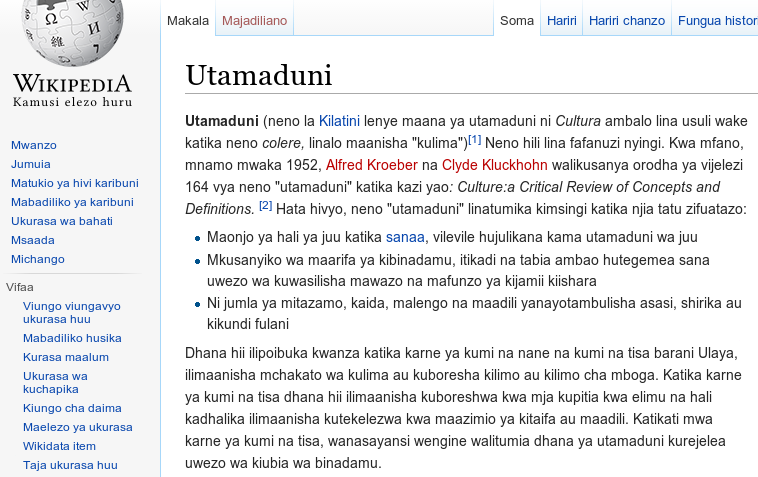
\includegraphics[keepaspectratio=true, scale=0.8]{./images/utamaduni-rom.png}
 % utamaduni_rom.png: 758x477 pixel, 96dpi, 20.05x12.62 cm, bb=0 0 568 358
 \caption{Part of the Swahili Wikipedia page on \textbf{utamaduni} (\textit{culture})}
 \label{fig:wikiR}
\end{figure}

Below are typeset versions of one paragraph in both scripts :

\begin{quotation}
Dhana hii ilipoibuka kwanza katika karne ya kumi na nane na kumi na tisa barani Ulaya, ilimaanisha mchakato wa kulima au kuboresha kilimo au kilimo cha mboga. Katika karne ya kumi na tisa dhana hii ilimaanisha kuboreshwa kwa mja kupitia kwa elimu na hali kadhalika ilimaanisha kutekelezwa kwa maazimio ya kitaifa au maadili. Katikati mwa karne ya kumi na tisa, wanasayansi wengine walitumia dhana ya utamaduni kurejelea uwezo wa kiubia wa binadamu.
\end{quotation}

\begin{quotation}
\begin{Arabic}
ذَانَ هِئِ إِلِپٗئِبُوكَ كْوَنْزَ كَتِيكَ كَارْنٖ يَ كُومِ نَ نَانٖ نَ كُومِ نَ تِيسَ بَرَانِ أُلَايَ، إِلِمَأَنِيشَ مْچَكَاتٗ وَ كُلِيمَ أَوْ كُبٗرٖيشَ كِلِيمٗ أَوْ كِلِيمٗ چَ مْبٗوڠَ۔ كَتِيكَ كَارْنٖ يَ كُومِ نَ تِيسَ ذَانَ هِئِ إِلِمَأَنِيشَ كُبٗرٖيشْوَ كْوَ مْجَ كُپِتِئَ كْوَ إٖلِيمُ نَ هَالِ كَذَلِيكَ إِلِمَأَنِيشَ كُتٖكٖلٖيزْوَ كْوَ مَأَزِمِؤٗ يَ كِتَئِيفَ أَوْ مَأَدِيلِ۔ كَتِكَاتِ مْوَ كَارْنٖ يَ كُومِ نَ تِيسَ، وَنَسَيَنْسِ وٖنْڠِينٖ وَلِتُمِئَ ذَانَ يَ أُتَمَدُونِ كُرٖجٖلٖئَ أُوٖيزٗ وَ كِؤُبِئَ وَ بِنَدَامُ۔
\end{Arabic}
\end{quotation}

\begin{figure}[H]
\centering
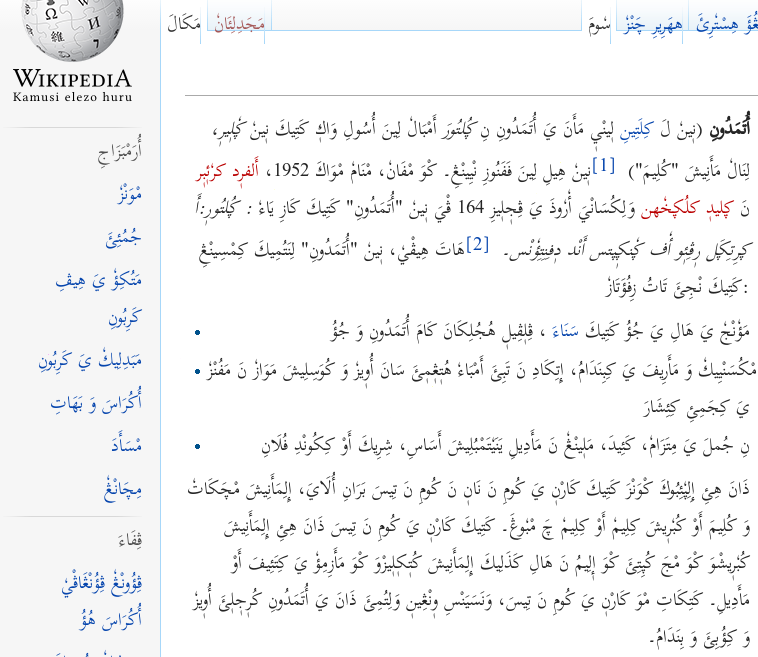
\includegraphics[keepaspectratio=true, scale=0.8]{./images/utamaduni-ar.png}
% utamaduni_ar.png: 758x657 pixel, 96dpi, 20.05x17.38 cm, bb=0 0 568 493
\caption{The page in \Cref{fig:wikiR} automatically transliterated into Arabic script}
\label{fig:wikiA}
\end{figure}

The following paragraph is from \citet{Hamad2011}, and is followed by an automatically-generated conversion to Arabic script.

\begin{quotation}
Mafanikio ya Siti yameelezwa kwa kufafanua matatizo aliyoyapata katika jamii yake katika kuendelea na hatua za kujinyanyua kiuchumi, hata hivyo alipambana nayo na aliweza kufanikiwa. Historia ya Siti imejitokeza kuwa ya kipekee kutokana na matendo yake katika jamii iliyo na utamaduni wa kuwaweka wanawake kutojitokeza hadharani hasa kwa kuimba kwa wakati huo. Siti akiwa mwanamke aliyepata misukosuko mbalimbali ya kukatisha tamaa katika maisha yake ikiwemo ya ndoa yake, aliweza kuhimili na kupambana nayo na kuweza kufikia kuwa mtu maarufu na wa kuheshimika ndani na hata nje ya mipaka ya jamii yake.
\end{quotation}

\begin{quotation}
\begin{Arabic}
مَفَنِكِؤٗ يَ سِيتِ يَمٖئٖلٖيزْوَ كْوَ كُفَفَنُؤَ مَتَتِيزٗ أَلِيٗيَپَاتَ كَتِيكَ جَمِئِ يَاكٖ كَتِيكَ كُئٖنْدٖلٖئَ نَ هَتُؤَ زَ كُجِنْيَنْيُؤَ كِؤُچُومِ، هَاتَ هِيڤْيٗ أَلِپَمْبَانَ نَايٗ نَ أَلِوٖيزَ كُفَنِكِيوَ۔ هِسْتٗرِئَ يَ سِيتِ إِمٖجِتٗكٖيزَ كُوَ يَ كِپٖكٖئٖ كُتٗكَانَ نَ مَتٖينْدٗ يَاكٖ كَتِيكَ جَمِئِ إِلِيٗ نَ أُتَمَدُونِ وَ كُوَوٖيكَ وَنَوَاكٖ كُتٗجِتٗكٖيزَ هَذَرَانِ هَاسَ كْوَ كُئِيمْبَ كْوَ وَكَاتِ هُؤٗ۔ سِيتِ أَكِيوَ مْوَنَامْكٖ أَلِيٖپَاتَ مِسُكٗسُوكٗ مْبَلِمْبَالِ يَ كُكَتِيشَ تَمَاءَ كَتِيكَ مَئِيشَ يَاكٖ إِكِوٖيمٗ يَ نْدٗؤَ يَاكٖ، أَلِوٖيزَ كُهِمِيلِ نَ كُپَمْبَانَ نَايٗ نَ كُوٖيزَ كُفِكِئَ كُوَ مْتُ مَأَرُوفُ نَ وَ كُهٖشِمِيكَ نْدَانِ نَ هَاتَ نْجٖ يَ مِپَاكَ يَ جَمِئِ يَاكٖ۔
\end{Arabic}
\end{quotation}


\section{Replicating prose in Arabic script}

The following is a copy of the specimen text from Appendix C of \citet{Omar1997}, which was included to show how their system would look in practice -- the text itself is from \citet{Omar1998}.  The conventions used here (eg the omission of short vowels in certain circumstances) differ slightly from those proposed in \textbf{Andika!} -- see \Cref{s:comparison} for further discussion.

\begin{quotation}
\begin{Arabic}
مار ٹُكَؤٗونَ مْليمَ أُنكِنڠام نديانِ، مْرٖيفُ سان۔  ٹُكَپانڈ؛ مْتانڠ واكٖ نِ وَ ذهابُ نَ ماوٖ ياكٖ نِ يَكوتِ نَ مرْجانِ۔  باسِ ٹُكَٹيكَ كْوٖينڈَ، مار ٹُكَؤٗونَ مْٹِ، سِجَؤٗونَ مْفانٗ واكٖ۔  تهين ياكٖ كونَ بَرٗبارٗ مْمٗوجَ أَتونڠَ نبوزِ، نَ هاءٗ نبوزِ پهٖيمب زاءٗ نِ زَ زُمُرودِ يَ كِجانِ كبيت، نَ مَنيٗؤَ ياءٗ نِ هَرير يَ رانڠِ كُلَّ نَمْنَ؛ مَزيوَ يَوتُرزيكَ، مٖؤوپٖ كام مَزيوَ يَ ميٹٗ يَ پهٖپٗونِ۔
 يَتٗوكَ كَٹيكَ: مَتٖمبٖيزِ يَ پهٖپٗونِ۔
\end{Arabic}
\end{quotation}

\begin{quotation}
Mara tukaona mlima unkingama ndiyani, mrefu sana.  Tukapanda; mtanga wake ni wa dhahabu na mawe yake ni yakuti na marjani.  Basi tukatika kwenda, mara tukaona mti, sijaona mfano wake.  T'ini yake kuna barobaro mmoja atunga mbuzi, na hao mbuzi p'embe zao ni za zumurudi ya kijani kibiti; na manyowa yao ni hariri ya rangi kulla namna; maziwa yawaturuzika, meupe kama maziwa ya mito ya P'eponi.
\end{quotation}

\begin{quotation}
\E{All of a sudden we saw a very high mountain which blocked the road.  So we climbed the mountain; its sand was like gold, and its stones were like rubies and seed-pearls.  Well then, as we continued on our way, we came across a tree the like of which I had never before seen.  Beneath it was a youth tending goats.  The horns of those goats were green like emeralds, and their silken fleeces were of divers colours, while their milk which dripped down was as white as the milk of the rivers of Paradise.}
\end{quotation}

\section{Replicating manuscript poetry: Bajuni fishing songs}
\Cref{fig:fishing} is part of a manuscript rendering of Bajuni fishing songs collected by Sheikh Yahya Ali Omar \citep{Donnelly1982}.  A letter-for-letter transcription of that follows, with an automatically-generated close transliteration in Roman script.  The Roman conversion uses various diacritics to reconcile the manuscript's representation of the Bajuni dialect with standard orthography.

\begin{figure}[ht]
\centering
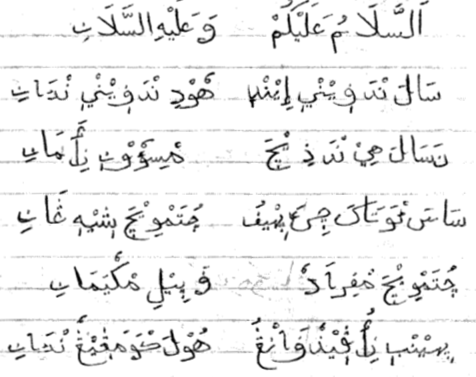
\includegraphics[keepaspectratio=true]{./images/fishing-orig.png}
% fishing_orig.png: 477x379 pixel, 100dpi, 12.12x9.63 cm, bb=0 0 343 273
\caption{Bajuni fishing songs as written out by Sheikh Yahya Ali Omar}
\label{fig:fishing}
\end{figure}

\begin{table}[H]
\begin{longtable}{r} 
\textarabic{اَلسَّلَامُ عَلَيْكُمْ * وَ عَلَيْهِ السَّلَانِ} \\* 
\Tr{assalāmu 'alaykum * wa 'alayhi assalāni} \\ 
\textarabic{سَالَ نْدَ ۏٖيْنْيٖ إِيْنْدٖ * هٗوْدِ نْدَ ۏٖيْنْيٖ نْدَانِ} \\* 
\Tr{sāla nḏa wēnye ı̄nḏe * hōḏi nḏa wēnye nḏāni} \\ 
\textarabic{نَ سَالَ هِيْ نْدَ ذِيْچَ * مْسِوٗوْنٖ نِأَمَانِ} \\* 
\Tr{na sāla hii nḏa ẕı̄tʲa * msiwōne niamāni} \\ 
\textarabic{سَاسَ ٹْوَتَاكَچِئَ پٖيْفُ * چُتَمْوِيْچَ شٖيْهٖ ڠَانِ} \\* 
\Tr{sāsa ţwaṯākatʲia pēfu * tʲuṯamwı̄tʲa shēhe gāni} \\ 
\textarabic{چُتَمْوِيْچَ مْفِراَدٗ * ۏَ پِيْلِ مْكٗيَمَانِ} \\* 
\Tr{tʲuṯamwı̄tʲa mfiraḏo * wa pı̄li mkoyamāni} \\ 
\textarabic{پٖيْنْبٖ نِ أُڤٖيْذٗ ۏَانْڠُ * هُوْلَ كْوَ مَڠٖيْڠٗ نْڈَانِ} \\* 
\Tr{pēm̱be ni uw̱ēẕo wāngu * hūla kwa magēgo nḑāni} \\ 
\end{longtable}
\end{table}

\begin{quotation}
\E{Peace to you, and to you peace.  The \textit{salaam} is for those outside, the \textit{hodi} is for those inside.  And this greeting is for war -- do not think it is for peace.  Now we will burn incense -- what learnèd man shall we call?  We'll call an Mfirado, and then a man from Koyamani.  A horn is my sign of strength -- I eat with molars inside.}
\end{quotation}


\section{Replicating manuscript poetry: Utenzi wa Mkunumbi}

\citet{Harries1967} is one of the few books of Swahili classical poetry to include the text in Arabic script in addition to the Roman transcription, in this case a photocopy of a copy made by Sheikh Yahya Ali Omar of the original manuscript . The Arabic script in that manuscript is less well-adapted to Swahili -- for instance, \textbf{o} is not used consistently.  \Cref{fig:mkunumbi} shows stanzas 3-5 of the \textit{utenzi}.

\begin{figure}[h]
 \centering
 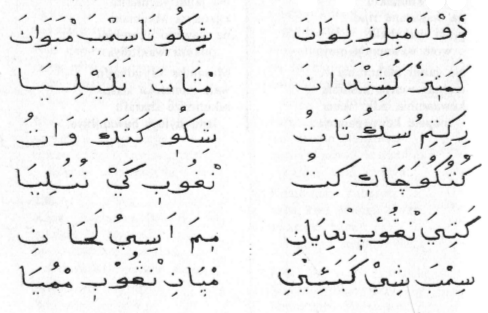
\includegraphics[keepaspectratio=true]{./images/mkunumbi.png}
 % mkunumbi.png: 488x313 pixel, 100dpi, 12.40x7.95 cm, bb=0 0 351 225
 \caption{Stanzas 3--5 of Utenzi wa Mkunumbi}
 \label{fig:mkunumbi}
\end{figure}

A letter-for-letter copy of the manuscript is shown below.  In this case the automatically-generated transcription was suppressed and replaced by Harries' own transcription, which was added manually and coloured green.

\begin{longtable}{rl}
\textarabic{دٗوْلَ مْبِلِ زِلِوَانَ * شِكُوٖ نَاسِمْبَ مْبَوَانَ} & \textarabic{٣} \\* 
\Swa{dola mbili zaliwana * Shekuwe na Simba Bwana} & \Tr{3a/b} \\
\textarabic{كَمَتٖزٗ كُشِنْدَانَ * مْتانَ نَلَيْلِيَ} &  \\* 
\Swa{kwa matezo kushindana * mtana na lailiya} & \Tr{3c/d} \\
\\[2mm] 

\textarabic{زِكِتِمُ سِكُ تَاتُ * شِكُوٖ كَتَكَ وَاتُ} & \textarabic{٤} \\* 
\Swa{zikitimu siku tatu * Shekuwe kataka watu} & \Tr{4a/b} \\
\textarabic{كُتُكُوَ چَاكٖ كِتُ * نْغُوبٖ كَيْ نُنُلِيَ} &  \\* 
\Swa{kutukua chake kitu * ng'ombe kainunuliya} & \Tr{4c/d} \\
\\[2mm] 

\textarabic{كَتِيَ نْڠُوْبٖ نْدِيَانِ * مٖمَ اَسِيُ لَحَانِ} & \textarabic{٥} \\* 
\Swa{katia ng'ombe ndiyani * mwema asio lahani} & \Tr{5a/b} \\
\textarabic{سِمْبَ شِيْ كَبَئِينِ * مْپَانِ نْڠُوبٖ مْمُيَ} &  \\* 
\Swa{Simba Shee kabaini * mbwanni ng'ombe mmoya} & \Tr{5c/d} \\
\end{longtable}

\begin{quotation}
\noindent\E{3. Two powers were in conflict / Shekuwe and Bwana Simba / opposing one another for sport / by day and by night.} \\
\E{4. When three days had passed / Shekuwe wanted men / to bring his offering / and he bought himself a cow.} \\
\E{5. And he sent the cow on the way / a good one without blemish / and Sheikh Simba observed it / [and said] What is the point of a single cow?}
\end{quotation}


An automatically-generated close transcription can be printed out separately if desired, as shown below.  In this case, an alternative layout has been selected, where the \textit{vipande} are each in their own column, instead of both being on one line.

\begin{longtable}{lll} 
\Tr{3a/b} & \Tr{ḏōla mbili ziliwāna} & \Tr{shikuwe nāsimba mbawāna} \\
\Tr{3c/d} & \Tr{kamaṯezo kushinḏāna} & \Tr{mṯāna nalayliya} \\
\\

\Tr{4a/b} & \Tr{zikiṯimu siku ṯāṯu} & \Tr{shikuwe kaṯaka wāṯu} \\
\Tr{4c/d} & \Tr{kuṯukuwa chāke kiṯu} & \Tr{nḡūbe kay nunuliya} \\
\\

\Tr{5a/b} & \Tr{kaṯiya ngūbe nḏiyāni} & \Tr{mema asiyu laḥāni} \\
\Tr{5c/d} & \Tr{simba shii kabaı̄ni} & \Tr{mpāni ngūbe mmuya} \\
\end{longtable}


\section{Replicating manuscript poetry: Kiswahili}

\citet{Abdulkadir2013} presents an annotated edition of the first author's poem, \AS{كِسْوَاحِلِ}.  It is rare among published work on Swahili in including the original Arabic script of the poem.  The following is a letter-for-letter transcription of stanza 4 of the author's manuscript as reproduced there, with the exception that the \textit{damma-with-tail} occasionally used by him to signify \textbf{o} is denoted here with \textit{inverted damma}, since the font does not yet include that glyph.  The full text of the poem is in Appendix D.

The layout includes an automatically-generated close and standard transliterations (the latter corrected manually where necessary), and the English translation and notes from the paper.  The Arabic text and the close transcription are set out in columns, so that the close transliteration relates directly to the \textit{kipande} above it, while the standard transliteration and the English translation are set out on a single line, so that they can be read in conjunction.  

Different fonts can be used for each layer of the text (the transliterations use sans serif fonts, while the translation uses a serif font in a smaller size), and each layer can be coloured (the standard transliteration is in green, while the close transliteration and translation are in shades of grey.  An epenthetic vowel has been added in blue in \textit{kipande} 4b.  The footnotes are marked in red and appear at the bottom of the page.  

\begin{longtable}{rrl}
\makebox[8cm][r]{} & & \makebox[8cm][r]{} \\ 
\textarabic{پِيَ مْوٖنْڠٗ عَثْمَانِ} & \textarabic{نْدِمِ مَامَاكٖ مُيَاكَ} & \textarabic{٤} \\* 
\Tr{piya mwengo 'ath}\In{u}\Tr{māni} & \Tr{nḏimi māmāke muyāka} & \\* 
\multicolumn{2}{r}{\Swa{ndimi mamake Muyaka\footnote{Bwana Muyaka was the outstanding Swahili poet of 19th century Mombasa.  After his death many of his verses were recalled by Mu'allim Sikujua Abdallah al-Batawi (died 1890) and transcribed with annotations by W.E. Taylor (1856-1927). After Taylor’s death his papers were acquired by the library of the School of Oriental and African Studies (SOAS), London.} * pia Mwengo Athumani\footnote{Mwengo Athmani: this 18th century poet from Pate composed the {\FN{Utendi wa Tambuka}} (\textit{The Epic of Heraklios}).}}} & \Swa{4a/b} \\* 
\multicolumn{2}{r}{\E{I am the mother of Bwana Muyaka, and of Mwengo Athmani also,}} & \\[2mm] 
\textarabic{نَ وٖنْڠِ وَاكٖ وٖنْدَانِ} & \textarabic{نَ زَهِدِ كَذَلِكَ} &  \\* 
\Tr{na wengi wāke wenḏāni} & \Tr{na zahiḏi kadhalika} & \\* 
\multicolumn{2}{r}{\Swa{na Zahidi\footnote{Zahidi: see El-Maawy (2008).} kadhalika * na wengi wake wendani}} & \Swa{4c/d} \\* 
\multicolumn{2}{r}{\E{and of Zahidi too, and many of his contemporaries,}} & \\[2mm] 
\textarabic{وٗتٖ مْبوَا مُوْيَ قَرِنِ} & \textarabic{عالى كُوْتِ نَ مَتَاكَ} &  \\* 
\Tr{woṯe mbwā mūya qarini} & \Tr{'ālı̄ kūṯi na maṯāka} & \\* 
\multicolumn{2}{r}{\Swa{Ali Koti\footnote{Ali Koti of Pate: see Chiraghdin (1987: 31-7).} na Mataka\footnote{Bwana Mataka’s full name is Muhammad bin Shee Mataka al-Famau (1825-1868). He was ruler of Siyu, as was his father. His mother was Mwana Kupona, famous for the poem of advice written to her daughter. Bwana Mataka died in Mombasa’s fort while imprisoned by the Busa‘idi.
} * wote mbwa moya karini}} & \Swa{4e/f} \\* 
\multicolumn{2}{r}{\E{Ali Koti and Mataka, all from just one century,}} & \\[2mm] 
\textarabic{وَ كَوَا كَمَ نْيوتَ} & \textarabic{وَلِتُوْكَ مَاتُوْمبونِ} &  \\* 
\Tr{wa kawā kama nı̄ūṯa} & \Tr{waliṯūka māṯūmbūni} & \\* 
\multicolumn{2}{r}{\Swa{walitoka matumboni * wakawaa kama nyota}} & \Swa{4g/h} \\* 
\multicolumn{2}{r}{\E{they emerged from my womb, and shone like stars.}} & \\[2mm] 
\end{longtable}



\chapter{Getting started}
\label{ch:started}

\section{Website}

The website\footnote{\url{kevindonnelly.org.uk/swahili}} allows you to experiment with \textbf{Andika!} regardless of the operating system (Microsoft Windows, Apple Mac OS, GNU/Linux, Android, etc) on your computer or device.  All you need to do is install the Scheherazade font\footnote{\url{scripts.sil.org/cms/scripts/page.php?item_id=Scheherazade}} so that all the Arabic glyphs (characters) used in Swahili are available.

In the Roman to Arabic section of the website you can type into a box in Roman script and have the input converted into Arabic script, or you can input a web address and have that whole page converted into Arabic script.  You can cut and paste the converted Arabic text into a word-processor.  The Arabic to Roman section of the website lets you convert Arabic script into standard Roman orthography.

\section{Introducing \textit{Ubuntu}}

The website offers only limited functionality -- to use \textbf{Andika!} fully, it is best to install it on your own computer.  \textbf{Andika!} was developed on GNU/Linux,\footnote{\url{en.wikipedia.org/wiki/Linux}} a free, secure, and versatile operating system which is not owned by any one company -- much of the internet runs on GNU/Linux, and large internet companies such as Google, Amazon and Facebook use it extensively.\footnote{Most of \textbf{Andika!} will work on Microsoft Windows or Apple Mac OS, but the crucial part (keyboard layout and activation) will not, since keyboard handling differs between operating systems -- I would be happy to accept appropriate layout files for operating systems other than GNU/Linux.}

The specific ``flavour'' of GNU/Linux used is Ubuntu.\footnote{ubuntu.com}  Ubuntu was started by a South African, Mark Shuttleworth, and the name is cognate with Swahili \AS{أُوتُ} (\textbf{utu}, \textit{humanity}), so it is apt for a project like \textbf{Andika!}  It is highly recommended to download Ubuntu\footnote{\url{ubuntu.com/download/desktop}} and install it\footnote{\url{ubuntu.com/download/desktop/install-ubuntu-desktop}} as your main operating system, but if that is not possible the next best thing is to run it in a virtual machine on top of Microsoft Windows or Apple Mac OS by installing VirtualBox\footnote{\url{virtualbox.org}} and then installing GNU/Linux into that.  Both these areas are outside the scope of this manual, but there is a wealth of information available on the internet about them.

Microsoft Windows or Apple Mac OS, which are owned by single companies, offer only a single desktop (interface to the operating system).  But with GNU/Linux is it possible to choose from a variety of desktops.  By default, Ubuntu comes with the Unity desktop\footnote{\url{unity.ubuntu.com}}, but the instructions here are mostly for the KDE desktop\footnote{\url{kde.org}}, since that is what I use.\footnote{I would be happy to include details for other desktops if anyone sends them to me.}  You can make KDE available by installing the \textit{kubuntu-desktop} package in Ubuntu, and you can then select either  the Unity or KDE desktop when the computer starts.

Detailed instructions for installing \textbf{Andika!} and the other software it requires are in \Cref{appA}.

\section{Typing Swahili in Arabic script}

If you simply want to type Swahili in Arabic script, it's very easy to get started:
\begin{enumerate}
\item Download \textbf{Andika!} (\ref{s:snapshot}) in a zip file.
\item Unzip the file.
\item Move into the \textit{andika} folder created.
\item Install the Scheherazade font so that all the Arabic glyphs (characters) used in Swahili are available (\ref{s:fonts}).
\item Install a keyboard so that the Arabic letters can be typed (\ref{s:keyboard}).
\item Configure the LibreOffice word-processor to handle Arabic script (\ref{s:libreoffice}).
\end{enumerate}

\section{Converting and annotating Swahili in Arabic script}

The above will not allow you to convert automatically from one script to the other -- for that you need to do the full installation in \Cref{appA}.  This will also allow you to transliterate, edit and annotate Swahili documents in Arabic script -- see \Cref{ch:poetry}.

\section{Next steps}

\Cref{ch:fonts} reviews some font-related issues.

\Cref{ch:keyboard} explains the keyboard layout used in \textbf{Andika!}, and how to access the various glyphs it caters for.

\Cref{ch:spelling} sets out proposed conventions for standard spelling of Swahili in Arabic script, which are used when converting between the standard Roman script and Arabic script and vice versa.

\Cref{ch:poetry} shows how Swahili poetry manuscripts in Arabic script can be transcribed to produce attractive output in various digital formats, including transliteration, translation, notes, emendations, variant readings, and so on, with the added benefit that the contents of the manuscripts are then available for computer analysis of language, vocabulary, word-frequency, etc.


\chapter{Fonts}
\label{ch:fonts}

\section{Missing glyphs in Arabic fonts}

In order to see Arabic script properly, the font you are using must contain Arabic glyphs (characters).  A number of fonts developed especially for Arabic are available,\footnote{For example, in the Ubuntu packages \textit{fonts-arabeyes} or \textit{fonts-kacst}, or on the web from the Open Font Library (\url{openfontlibrary.org/en/search?query=Arabic}).} but many of them contain only the glyphs needed to write standard Arabic.

If you are using \textbf{Andika!} to transcribe manuscripts, it may be that these glyphs will be all you need, since many Swahili writers in the past used the Arabic script to provide only an approximation to the Swahili sounds, and depended on the linguistic knowledge of native speakers to interpret the text correctly \citep[p14-15]{Omar2002}.\footnote{The examples are: \AS{نِغِمَا وَغُ بِنْتِ} (\textit{negema wangu binti}), \AS{يِيِ كِيَ مُولَ وَكُ} (\textit{nyenyekea Mola wako}), and \AS{مْتُ هُنِنَ اَكِرَ * اَسِيَابَرَكِ تَرَ} (\textit{mtu hunena akenda * asiyapanda kitanda})}

However, if you are using the spelling conventions proposed in \textbf{Andika!} in order to unambiguously represent current-day Swahili, and allow transliteration between Arabic script and the standard Swahili Roman script, then you will need the additional glyphs.  If you see squares or boxes in the Arabic script, or just the glyph for the isolated form when initial, medial or final forms are required, the reason is that the font you are using is missing the glyphs that it would make it useable with Swahili.

The missing glyphs are likely to be one or more of those in \Cref{tab:missglyphs}.  The first seven glyphs are the most important.
\begin{table}[h!]
\centering
\begin{tabularx}{14cm}{llll}
\textbf{Glyph} & \textbf{Unicode name} & \textbf{Unicode number} & \textbf{Notes} \\
\hline\noalign{\smallskip}
\AS{پ} & peh & U+067E & \textbf{p} \\
\AS{ڤ} & veh & U+06A4 & \textbf{v} \\
\AS{چ} & tcheh & U+0686 & \textbf{ch} \\
\AS{ڠ} & ain with three dots above & U+06A0 & \textbf{g} \\
\AS{ݝ} & ain with two dots above & U+075D & \textbf{g} in \textbf{ng'} \\
\AS{ٖ} & subscript alef & U+0656 & short \textbf{e} \\
\AS{ٗ} & inverted damma & U+0657 & short \textbf{o} \\
\AS{\char"063B} & keheh with two dots above & U+063B & used by some writers for \textbf{ch} \\  % entering keheh from the keyboard won't work -- the codepoint seems not to be in Linux Biolinum
\AS{ٹ} & tteh & U+0679 & alveolar \textbf{t} (Mombasa) \\
\AS{ڈ} & ddal & U+0688 & alveolar \textbf{d} (Mombasa) \\
\AS{ۏ} & waw with dot above & U+06CF & \textbf{w} (North) \\
\AS{ژ} & jeh & U+0698 & \textbf{zh} (North) \\
\end{tabularx}
\caption{Glyphs commonly missing in fonts}
\label{tab:missglyphs}
\end{table}

At the time of writing, the only fonts which contain all of these additional glyphs in \Cref{tab:missglyphs} are Scheherazade\footnote{\url{scripts.sil.org/cms/scripts/page.php?item_id=Scheherazade}, available in the Ubuntu package \textit{fonts-sil-scheherazade}, but see also \Cref{s:fonts}.} (by Bob Hallissy and Jonathan Kew), Amiri\footnote{\url{amirifont.org}} (by Khaled Hosny), and the fonts from the PakType project.\footnote{\url{paktype.sourceforge.net}, available in the Ubuntu package \textit{fonts-paktype}.}

Fonts containing all the glyphs in \Cref{tab:missglyphs} apart from \textit{keheh} are Droid Arabic Naskh\footnote{\url{openfontlibrary.org/en/font/droid-arabic-naskh}} and Droid Arabic Kufi\footnote{\url{openfontlibrary.org/en/font/droid-arabic-kufi}} (by Pascal Zoghbi), and Lateef.\footnote{\url{scripts.sil.org/cms/scripts/page.php?item_id=Lateef}}

\section{Default fonts in \textbf{Andika!}}
\label{s:changefont}

When typing Swahili in Arabic script, the fonts can be changed directly in LibreOffice.  For typesetting of existing manuscripts,  \textbf{Andika!} uses four fonts as defaults when generating pdfs:
\begin{itemize}
\item Scheherazade for the Arabic transcription.  A possible alternative here is Amiri.
\item Linux Biolinum O\footnote{\url{linuxlibertine.org}} for the close transcription into Roman script, since it is especially good at handling diacritics.  A possible serif alternative here is Gentium\footnote{\url{scripts.sil.org/cms/scripts/page.php?site_id=nrsi&item_id=Gentium}} (by Victor Gaultney).
\item Liberation Serif\footnote{\url{fedorahosted.org/liberation-fonts}} for English translations.
\item GranadaKD in \textit{andika/fonts} for poem titles in Arabic.  This is a Kufic-style font from Arabeyes\footnote{\url{openfontlibrary.org/en/font/granada}} that has been adapted by me to add the characters in \Cref{tab:missglyphs} except \textit{keheh}.
\end{itemize}

These default fonts can be changed by replacing the name of the font in the relevant command in \textit{poetry/tex/poem\_header.tex}.  Thus, to change the transliteration font from Linux Biolinum O to Gentium, you would first install Gentium:

\verb|sudo apt-get install fonts-sil-gentium|

and then open \textit{poetry/tex/poem\_header.tex} in a text-editor\footnote{A text-editor is an application specialising in the editing of text.  Word-processors should never be used to edit files in \textbf{Andika!}, because they will quietly change the file in ways which will prevent it working.  There are multiple text-editors such as Kate, Geany, and Gedit available in Ubuntu.} and change the line:

\verb|\newcommand\Tr[1]{{\fontspec[Scale=1, Color=666666]{Linux Biolinum O}#1}}|

to:

\verb|\newcommand\Tr[1]{{\fontspec[Scale=1, Color=666666]{Gentium}#1}}|

The \textit{Color} command sets the colour of the font using the hex version of the RGB value \footnote{\url{colorspire.com/rgb-color-wheel}} (in this case, dark grey) -- delete it if you want the transliteration in black.  The \textit{Scale} command alters the size of the font -- if you want it a bit smaller than normal, enter (say) 0.8 instead of 1.

As a general point, the readability of diacritics (or even whether they are displayed at all) depends crucially on the font -- not all will be capable of showing all diacritics, or of placing them in the right location, so if something is not looking right in your transliteration, try using Linux Biolinum O (sans-serif) or Gentium (serif) as suggested. 

\section{Adding missing glyphs to Arabic fonts}

If you are anxious to use a particular Arabic font that does not have all the glyphs required by Swahili, it is possible to add them to the font using the font editor FontForge,\footnote{\url{fontforge.github.io}} originally developed by George Williams.  \Cref{appB} shows how to use FontForge to add missing glyphs,\footnote{Note that unless the font you are adapting is available under an open license, it is a breach of copyright to distribute the adapted font.} but note that this will require some commitment of time, since FontForge is a complex program.

You can also develop your own fonts using FontForge, though the creation of an attractive font is a highly specialised task requiring artistic flair as well as technical skill.   There is a detailed tutorial on FontForge,\footnote{\url{designwithfontforge.com}} and the drawing program Inkscape\footnote{\url{inkscape.org}} now allows initial glyph designs to be created there and then imported into FontForge for finalisation.\footnote{\url{understandingfonts.com/blog/2011/11/typography-extensions-in-inkscape-0-49}}  (This functionality is expected in the next version, 0.49, but in the meantime it can be accessed by using the ``bleeding edge'' packages available from Inkscape Trunk.\footnote{\url{launchpad.net/~inkscape.dev/+archive/ubuntu/trunk}})

\section{Scheherazade and Amiri}
\label{s:sham}

The Scheherazade webpage\footnote{\url{scripts.sil.org/cms/scripts/page.php?item_id=Scheherazade}} notes that:
\begin{quotation}
Scheherazade provides a “simplified” rendering of Arabic script, using basic connecting glyphs but not including a wide variety of additional ligatures or contextual alternates (only the required lam-alef ligatures). This simplified style is often preferred for clarity, especially in non-Arabic languages, but may not be considered appropriate in situations where a more elaborate style of calligraphy is preferred.
\end{quotation}

Scheherazade is the default in \textbf{Andika!} because it fits the proposed full vocalisation better.  For instance, Amiri places all the vowels at the same height from the main letter, eg \Am{كُبٗرٖيشَ} (\textit{kuboresha}, to boost) compared to Scheherazade \AS{كُبٗرٖيشَ}, and \Am{وَنَسَيَانْسِ} (\textit{wanasayansi}, scientists) compared to Scheherazade \AS{وَنَسيَانْسِ}. This can lead to the upper vowels from the current line of text colliding with the lower vowels from the previous line.

However, Amiri may be more appropriate for use with text that is not fully vocalised (eg quotation of Arabic within Swahili), particularly since it includes more of the ligatures commonly used in Arabic, making for more attractive text. For instance, Amiri \Am{وَلِتُمئَِ} (\textit{walitumia}, they used), compared to Scheherazade \AS{وَلِتُمئَِ}, has the letters \textit{ltm} combined in one ligature.


\chapter{A keyboard layout for Swahili in Arabic script}
\label{ch:keyboard}

\section{Introduction}

The keyboard layout proposed here is a work-in-progress, and can be adjusted in the light of experience -- I would be happy to receive any suggestions for improvement.  As well as describing the keyboard and explaining the conventions governing the layout, this chapter also includes information on how to edit the layout to suit individual needs.

The \textbf{Andika!} keyboard allows Swahili in Arabic script to be typed directly into a GNU/Linux computer using a standard English (UK or US) keyboard. Input speed is comparable to typing in Roman script.  As well as allowing contemporary Swahili to be easily typed in Arabic script, the keyboard will enable most older manuscripts to be transliterated letter-for-letter.

The complete keyboard layout is depicted in \Cref{fig:kblayout}.\footnote{I am grateful to Wikimedia for the original layout image.} 

\begin{figure}[!ht]
 \centering
 \includegraphics[keepaspectratio=true, scale=0.7]{./images/Swahili-keyboard.png}
 % Swahili_keyboard.png: 797x246 pixel, 90dpi, 22.50x6.94 cm, bb=0 0 638 197
 \caption{Keyboard layout for writing Swahili in Arabic script}
 \label{fig:kblayout}
\end{figure}

As can be seen from Figure \ref{fig:kblayout}, up to four glyphs may be accessed from one key.  To access the contents of each key, the \textbf{Shift} and \textbf{AltGr} keys are used in combination where appropriate, as shown in \Cref{fig:key}.

\begin{figure}[!ht]
 \centering
 \includegraphics[keepaspectratio=true, scale=1]{./images/key.png}
 % key.png: 562x100 pixel, 90dpi, 15.86x2.82 cm, bb=0 0 450 80
 \caption{Accessing the glyphs on the keys}
 \label{fig:key}
\end{figure}

\section{Governing principles for the layout}

The basic governing principle behind the keyboard layout is that the relevant Arabic glyph will usually be produced by pressing the same key that produces the Roman glyph.  It is thus very easy to use: just switch your keyboard to use Arabic script -- in KDE, \textbf{Ctrl+Alt+K} (see \Cref{s:kbactivate} for further information) -- and start typing almost as if the keyboard is being used to type Roman script.  Some examples are given in \Cref{tab:typeeg}.\footnote{For an explanation of the penultimate long vowels accessed by the Shift keys, see \Cref{ch:spelling}.}

\begin{table}[h!]
\centering
\begin{tabularx}{10cm}{rlll}
\textbf{Arabic} & \textbf{Keystrokes} & \textbf{Roman} & \textbf{English}\\
\hline\noalign{\smallskip}
\AS{مِيمِ} & m, i, Shift+i, m, i & mimi & I, me \\
\AS{سَاسَ} & s, a, Shift+a, s, a & sasa & now \\
\AS{لَكِينِ} & l, a, k, i, Shift+i, n, i & lakini & but \\
\AS{نِمٖفِيكَ} & n, i, m, e, f, i, Shift+i, k, a & nimefika & I have arrived \\
\end{tabularx}
\caption{Typing examples}
\label{tab:typeeg}
\end{table}

The other main principle behind the layout is the consistent placement of glyphs that are related by shape or sound in either script:
\begin{itemize}
\item The digraphs \textbf{dh gh th sh zh} are on the same keys as \textbf{d g t s z}, and are accessed using the \textbf{Shift} key.
\item The pharyngeal consonants \AS{ص ض ط ظ} are on the same keys as \textbf{z t d s}, and are accessed using the \textbf{AltGr} key.
\item Similar Arabic glyph shapes are placed on the same key where possible -- for instance \AS{ي ى} are on the \textbf{y} key, and \AS{و ۏ} are on the \textbf{w} key.
\item Long and short vowels are located on the same key, with the long vowel accessed by \textbf{Shift}, so for instance the \textbf{u} key produces \AS{ُ } and \textbf{Shift+u} produces \AS{و}.
\item The vowel carriers \AS{أ إ ئ ؤ} are all accessed using the\textbf{AltGr} key.
\item The alveolar consonants \AS{ٹ ڈ} used in Mombasa Swahili are accessed using the \textbf{AltGr+Shift} keys.
\item The glyphs \AS{و ي} are repeated on \textbf{w y} for use when they represent semi-vowels.
\item The palatal digraph \textbf{ch} is accessed using the \textbf{c} key, and an alternate representation used by some writers, \AS{\char"063B}, is accessed using \textbf{Shift+c}.
\item The occasionally-used digraph \textbf{kh} is accessed using the \textbf{X} key.
\item Non-alphabetic characters from the UK keyboard are currently available via \textbf{AltGr} and \textbf{AltGr+Shift}, in case they might be of use.
\end{itemize}

Further information on the glyphs accessible from each key is available in \Cref{tab:consonants} (consonants) and \Cref{tab:vowels} (vowels).

\section{Changing the layout}
\label{s:changelayout}

The layout of the keyboard is specified in the file \textit{layout/tz}.  Once copied to the appropriate place (see \Cref{s:keyboard}), the layout is available for use.  The file (reproduced in \Cref{appE}) is a simple text file, and can be easily adapted to add new glyphs or change the position of existing glyphs -- see \Cref{appC} for instructions on doing this.



\chapter{Writing contemporary Swahili in Arabic script}
\label{ch:spelling}

\section{Introduction}

The spelling conventions suggested here for writing contemporary Swahili in Arabic script are based on those developed by Sheikh Yahya Ali Omar, as evidenced in his own manuscripts and in \citet{Omar1997}.  However, I am wholly responsible for the conventions set out here, and for any unwitting misinterpretation!  In particular, the issue of vowel sequences\footnote{I have tried to build on the discussion in \citet{Omar1997}: \textit{Appendix B: The Hamza in Swahili Arabic script}.} (\Cref{s:vseq} below) is a complex one, and may need revision based on input from first-language speakers who are literate in Swahili in Arabic script. I would be happy to hear from anyone who has any comments on the conventions.

\section{General principles}

Word segmentation is as for standard Swahili in Roman script. This means that items such as \AS{لَ زَ يَ نَ} \textbf{na, ya, za, la} are written separately from the following word, even though in older manuscripts they may be written attached to that word.

All short vowels are marked. Although short vowels are usually omitted in Arabic, this is inadvisable in Swahili because of the different structure of the language, and also because Swahili has five vowels instead of three.

The penultimate syllable of a word has its stress marked by writing it with a long vowel. \AS{ا} is used for \textbf{a}, \AS{ي} for \textbf{e} and \textbf{i}, and \AS{و} for \textbf{o} and \textbf{u}.\footnote{The short vowels \textbf{a, i, u} may be omitted when they occur before a long vowel, eg \AS{ساسَ} instead of \AS{سَاسَ} (\textbf{sasa}, \textit{now}), but this is not recommended.} This also helps to delimit individual words in the Arabic script.

Initial vowels use the vowel-carriers \AS{أ} (\textbf{AltGr+A}, for \textbf{a, o, u}) or \AS{إ} (\textbf{AltGr+\textbackslash}, for \textbf{e, i}), eg \AS{أَنَسٖيمَ} (\textbf{anasema}, \textit{he is speaking}), \AS{أُڠَالِ} (\textbf{ugali}, \textit{porridge}), \AS{إِذِينِ} (\textbf{idhini}, \textit{permission}).\footnote{\citet[p69]{Omar1997} recommends omission of the \textit{hamza}, presumably in order to limit the number of diacritics in the text, but the current convention in \textbf{Andika!} is to write it.} The order of typing is: vowel carrier, then short vowel, then long vowel (if applicable).

Arabic sounds in loanwords should ideally use the original Arabic glyph, but they can also be written as an Arabic transliteration of the Roman letter, eg \AS{ذ} instead of \AS{ض} or \AS{ظ}.\footnote{Note that the Roman to Arabic converter will always do this, since standard Swahili in Roman script does not preserve these distinctions.}


\section{Representation of consonants}

The representation of Swahili vowels in Arabic script is set out in \Cref{tab:consonants}.

\begin{longtable}[c]{p{4cm}rp{3cm}rp{5cm}}  % [c] means the table will be centered.
\textbf{Roman} & \textbf{Arabic} & \textbf{Keystrokes} & & \textbf{Example} \\
\noalign{\bigskip}\hline\noalign{\bigskip}

b & \AS{ب} & b & \AS{كِبُورِ} & ki\textbf{b}uri (\textit{arrogance}) \\
\noalign{\medskip}

ch & \AS{چ} & c & \AS{چُونڠوَ} & \textbf{ch}ungwa (\textit{large orange}) \\
\noalign{\medskip}
ch (aspirated, Mombasa) & \AS{چه} & c, h & \AS{چهُونڠوَ} & \textbf{ch'}ungwa (\textit{medium-sized orange}) \\
\noalign{\medskip}

d & \AS{د} & d & \AS{كُدَنڠَانيَ} & ku\textbf{d}anganya (\textit{to deceive}) \\
\noalign{\medskip}
d - alveolar d (Mombasa) & \AS{ڈ} & AltGr+Shift+d & \AS{ٹُونڈُ} & tun\textbf{d}u (\textit{chicken coop}) \\
\noalign{\medskip}
dh & \AS{ذ} & Shift+d & \AS{ذَهَابُ} & \textbf{dh}ahabu (\textit{gold}) \\
\noalign{\medskip}
dh (pharyngeal) & \AS{ض} & AltGr+d & \AS{ضِيكِ} & \textbf{dh}iki (\textit{distress}) \\
\noalign{\medskip}
dh (pharyngeal) & \AS{ظ} & AltGr+z & \AS{أَظُهُورِ} & a\textbf{dh}uhuri (\textit{noon}) \\
\noalign{\medskip}

f & \AS{ف} & f & \AS{فِيڠٗ} & \textbf{f}igo (\textit{kidneys}) \\
\noalign{\medskip}

g & \AS{ڠ} & g & \AS{ڠُنِئَ} & \textbf{g}unia (\textit{sack}) \\
\noalign{\medskip}
gh & \AS{غ} & h & \AS{غَضَابُ} & \textbf{gh}adhabu (\textit{anger}) \\
\noalign{\medskip}

h & \AS{ه} & h & \AS{هَاكٗ} & \textbf{h}ako (\textit{he is not here}) \\
\noalign{\medskip}
h (pharyngeal) & \AS{ح} & Shift+h & \AS{حَسَن} & \textbf{H}asan (\textit{Hasan} [name]) \\
\noalign{\medskip}
[k]h & \AS{خ} & x & \AS{خَبَارِ} & \textbf{[k]h}abari (\textit{news}) \\
\noalign{\medskip}

j & \AS{ج} & j & \AS{جَانَ} & \textbf{j}ana (\textit{yesterday}) \\
\noalign{\medskip}

k & \AS{ك} & k & \AS{كُوكُ} & \textbf{k}u\textbf{k}u (\textit{large hen}) \\
\noalign{\medskip}
k (aspirated, Mombasa) & \AS{كه} & k, h & \AS{كهُوكُ} & \textbf{k'}uku (\textit{medium-sized hen}) \\
\noalign{\medskip}

l & \AS{ل} & l & \AS{كُلِيمَ} & ku\textbf{l}ima (\textit{to dig}) \\
\noalign{\medskip}

m & \AS{م} & m & \AS{مِيمِ} & \textbf{m}imi (\textit{I}) \\
\noalign{\medskip}
% m , Shift+ . (full stop) & \AS{مْ} & m - syllabic (eg Classes 1 and 3) & \AS{مْپٖينزِ} & \textbf{m}penzi (\textit{beloved}) \\

n & \AS{ن} & n & \AS{نَانِ} & \textbf{n}a\textbf{n}i (\textit{who?}) \\
\noalign{\medskip}
ng' & \AS{نݝ} & n, Shift+n & \AS{نݝٗومبٖ} & \textbf{ng'}ombe (\textit{cattle}) \\
\noalign{\medskip}

p & \AS{پ} & p & \AS{كُپَاكَ} & ku\textbf{p}aka (\textit{to paint}) \\
\noalign{\medskip}

q & \AS{ق} & q & \AS{وَقْفُ} & wa\textbf{q}fu (\textit{consecrated}) \\
\noalign{\medskip}

r & \AS{ر} & r & \AS{كُرُودِ} & ku\textbf{r}udi (\textit{to come back}) \\
\noalign{\medskip}

s & \AS{س} & s & \AS{كُسِمَامَ} & ku\textbf{s}imama (\textit{to stand}) \\
\noalign{\medskip}
s (pharyngeal) & \AS{ص} & AltGr+s & \AS{صَحِيبُ} & \textbf{s}ahibu (\textit{friend}) \\
\noalign{\medskip}
sh & \AS{ش} & Shift+s & \AS{كُشِيكَ} & ku\textbf{sh}ika (\textit{to hold}) \\
\noalign{\medskip}

t & \AS{ت} & t & \AS{فِتِينَ} & fi\textbf{t}ina (\textit{intrigue}) \\
\noalign{\medskip}
t (aspirated dental, Mombasa) & \AS{ته} & t, h & \AS{تهُوپَ} & \textbf{t'}upa (\textit{bottle}) \\
\noalign{\medskip}
t (alveolar, Mombasa) & \AS{ٹ} & AltGr+Shift+t & \AS{ٹُونڈُ} & \textbf{t}undu (\textit{chicken coop}) \\
\noalign{\medskip}
t (pharyngeal) & \AS{ط} & t & \AS{كُطَهِرِيشَ} & ku\textbf{t}ahirisha (\textit{to purify}) \\
\noalign{\medskip}
th & \AS{ث} & Shift+t & \AS{ثَمَنِينِ} & \textbf{th}amanini (\textit{eighty}) \\
\noalign{\medskip}

v & \AS{ڤ} & v & \AS{كُڤِيمبَ} & ku\textbf{v}imba (\textit{to swell}) \\
\noalign{\medskip}

z & \AS{ز} & z & \AS{كُزِيمَ} & ku\textbf{z}ima (\textit{to extinguish}) \\
\noalign{\medskip}
zh (Northern) & \AS{ژ} & Shift+z & \AS{ژِينَ} & \textbf{zh}ina (\textit{name}) \\
\noalign{\medskip}

w & \AS{و} & w & \AS{كُوَ} & ku\textbf{w}a (\textit{to be}) \\
\noalign{\medskip}
w (labio-dental) & \AS{ۏ} & AltGr+Shift+w & \AS{ۏِينٗ} & \textbf{w}ino (\textit{ink}) \\
\noalign{\medskip}

y & \AS{ي} & y & \AS{يَاكٗ} & \textbf{y}ako (\textit{your}) \\
\noalign{\medskip}

ʕ (pharyngeal) & \AS{ع} & ` (single quote) & \AS{مَعَانَ} & ma\textbf{'}ana (\textit{meaning}) \\
\noalign{\medskip}

\textit{hamza} (vowel-carrier) & \AS{ء} & AltGr+Shift+h & \AS{تَاءٗ} & ta\textbf{o} (\textit{arch}) \\
\noalign{\medskip}

\textit{hamza} (marks long vowels used as vowel-carriers) & \AS{ٔ} & Shift+ , (comma) & \AS{كُپِكِئَ} & kupik\textbf{i}a (\textit{to cook for}) \\
\noalign{\medskip}

\textit{sakani} (marks a consonant without a following vowel) & \AS{ْ} & Shift+ . (full stop) & \AS{أَسْلَارِ} & a\textbf{s}kari (\textit{soldier}) \\
\noalign{\medskip}

\textit{shada} (marks a doubled consonant in Arabic words) & \AS{ّ} & Shift+ ` (single quote) & \AS{وَالنَّهَارِ} & wa-\textbf{nn}ahari (\textit{and day}) \\
\noalign{\bigskip}\hline\noalign{\bigskip}

\multicolumn{5}{p{12cm}}{\textbf{NOTE}: In the \textbf{Keystrokes} column, the comma stands for \textit{followed by}.} \\
% can't use quotes in the multicolumn field.
\noalign{\bigskip}

\caption{Representation of consonants}\\
\label{tab:consonants}
\end{longtable}



\section{Representation of vowels}

The representation of Swahili vowels in Arabic script is set out in \Cref{tab:vowels}.

\begin{longtable}[c]{p{1.5cm}rp{2cm}rp{5cm}}  % [c] means the table will be centered.
\textbf{Roman} & \textbf{Arabic} & \textbf{Keystrokes} & & \textbf{Example} \\
\noalign{\bigskip}\hline\noalign{\bigskip}

a-...  & \AS{أَ} & AltGr+a, a & \AS{أَسٗومَ} & \textbf{a}soma (\textit{he reads}) \\
\noalign{\medskip}
...-a-... & \AS{َ} &a & \AS{بَهَرِينِ} & b\textbf{a}h\textbf{a}rini (\textit{in the sea}) \\
\noalign{\medskip}
...-a\CV{CV} & \AS{َ  ا} & a, Shift+a & \AS{سَاسَ} & s\textbf{a}sa (\textit{now}) \\
\noalign{\medskip}
...-a\CV{V} & \AS{َ   ا ء} & a, Shift+a,  & \AS{مَفَاءَ} & maf\textbf{a}a (\textit{usefulness}) \\
&& AltGr+Shift+h & \AS{تَاءِ} & t\textbf{a}i \textit{(vulture)} \\
&&& \AS{بَاءٗ} & b\textbf{a}o \textit{(plank)} \\
\noalign{\bigskip}\hline\noalign{\bigskip}

e-...  & \AS{إٖ} & AltGr+\textbackslash, e & \AS{إٖندٖلٖئَ} & \textbf{e}ndelea (\textit{go on!}) \\
\noalign{\medskip}
...-e-... & \AS{ٖ} & e & \AS{كٖلٖيلٖ} & k\textbf{e}lel\textbf{e} (\textit{shout}) \\
\noalign{\medskip}
...-e\CV{CV} & \AS{ٖ ي} & e, Shift+e & \AS{نجٖيمَ} & nj\textbf{e}ma (\textit{good}) \\
\noalign{\medskip}
...-e\CV{V} & \AS{ٖ ئ} & e, AltGr+e & \AS{كُپٖئَ} & kup\textbf{e}a (\textit{to sweep}) \\
&&& \AS{كُپٗكٖئَ} & kupok\textbf{e}a \textit{(plank)} \\
\noalign{\bigskip}\hline\noalign{\bigskip}

i-...  & \AS{إِ} & AltGr+\textbackslash, i & \AS{إِسِپٗكُوَ} & \textbf{i}sipokuwa (\textit{unless}) \\
\noalign{\medskip}
...-i-... & \AS{ِ} & i & \AS{كِتَابُ} & k\textbf{i}tabu (\textit{book}) \\
\noalign{\medskip}
...-i\CV{CV} & \AS{ِ  ي} & i, Shift+i & \AS{مَشِيزِ} & mash\textbf{i}zi (\textit{soot}) \\
\noalign{\medskip}
...-i\CV{V} & \AS{ِ  ئ} & i, AltGr+i & \AS{كُتِئَ} & kut\textbf{i}a (\textit{to place}) \\
\noalign{\bigskip}\hline\noalign{\bigskip}

o-...  & \AS{أٗ} & AltGr+a, o & \AS{أٗكتٗوبَ} & \textbf{O}ktoba (\textit{Oktober}) \\
\noalign{\medskip}
...-o-... & \AS{ٗ} & o & \AS{كِلِيمٗ} & kilim\textbf{o} (\textit{cultivation}) \\
\noalign{\medskip}
...-o\CV{CV} & \AS{ٗ  و} & o, Shift+o & \AS{مْكٗونڠَ} & mk\textbf{o}nga (\textit{elephant's trunk}) \\
\noalign{\medskip}
...-o\CV{V} & \AS{ٗ  ؤ} & o, AltGr+o & \AS{كُپٗؤَ} & kup\textbf{o}a (\textit{to cool}) \\
\noalign{\bigskip}\hline\noalign{\bigskip}

u-...  & \AS{أُ} & AltGr+a, u & \AS{أُلِيمِ} & \textbf{u}limi (\textit{tongue}) \\
\noalign{\medskip}
...-u-... & \AS{ُ} & u & \AS{كُشُكُورُ} & k\textbf{u}sh\textbf{u}kur\textbf{u} (\textit{ to give thanks}) \\
\noalign{\medskip}
...-u\CV{CV} & \AS{ُ  و} & u, Shift+u & \AS{كُومِ} & k\textbf{u}mi (\textit{ten}) \\
\noalign{\medskip}
...-u\CV{V} & \AS{ُ  ؤ} & u, AltGr+u & \AS{كُسُڠُؤَ} & kusug\textbf{u}a (\textit{to rub}) \\
\noalign{\bigskip}\hline\noalign{\bigskip}

\multicolumn{5}{p{12cm}}{\textbf{NOTE}: In the \textbf{Roman} column, \CV{C} stands for \textit{consonant} or \textit{consonant cluster} and \CV{V} for \textit{vowel}, and the entries refer respectively to (1) non-initial, (2) non-initial and non-penultimate, (3) penultimate followed by a consonant, (4) penultimate followed by a vowel.  For a discussion of vowel-sequences, see \Cref{s:vseq}.  In the \textbf{Keystrokes} column, the comma stands for \textit{followed by}.} \\
\noalign{\bigskip}

\caption{Representation of single vowels}
\label{tab:vowels}
\end{longtable}

\section{Vowel sequences}
\label{s:vseq}

Vowel sequences have matching vowel-carriers inserted between them, as set out in \Cref{tab:carriers}.

\begin{longtable}[c]{p{2cm}p{2cm}rp{4.5cm}}  % [c] means the table will be centered.
\textbf{Vowel} & \textbf{Carrier} & \textbf{Arabic} & \textbf{Keystrokes} \\
\noalign{\smallskip}\hline\noalign{\smallskip}
e, i & \textit{yeh+hamza} & \AS{ئ} & AltGr+Shift+I or E or Y \\
\noalign{\medskip}
o, u & \textit{waw+hamza} & \AS{ؤ} & AltGr+Shift+O or U or W \\
\noalign{\medskip}
a & \textit{alef+hamza} & \AS{ا ء} or \AS{أ}& Shift+A, AltGr+Shift+H\\
\noalign{\bigskip}
\caption{Vowel-carriers}
\label{tab:carriers}
\end{longtable}

\subsection{Stressed+unstressed vowel sequences}

When the vowel is first in the vowel sequence and is also stressed (which will only happen when it is in penultimate position in the word), a vowel-carrier is inserted after it.  Where \textbf{a} is concerned, the \textit{hamza} on the carrier is written as a full letter rather than a diacritic.

\hangindent=3cm  % controls the amount of indentation from left (positive value) or right (negative value).
\hangafter=0  % controls the number of full-width lines before/after changing the indent (\hangindent) - a positive number produces full-width lines at the beginning, whereas a negative number produces them at the end. 0 means we want them all indented, including the first line.
\textbf{kupea} (\textit{to sweep}) \textrightarrow\ kupe\SPSB{\AS{ء}}{y}a \textrightarrow\ \AS{كُپٖئَ} \\
\textbf{kupokea} (\textit{to receive}) \textrightarrow\ kupoke\SPSB{\AS{ء}}{y}a \textrightarrow\ \AS{كُپٗكٖئَ} \\
\textbf{kutia} (\textit{to place}) \textrightarrow\ kuti\SPSB{\AS{ء}}{y}a \textrightarrow\ \AS{كُتِئَ} \\
\textbf{kupoa} (\textit{to cool}) \textrightarrow\ kupo\SPSB{\AS{ء}}{w}a \textrightarrow\ \AS{كُپٗؤَ} \\
\textbf{kusugua} (\textit{to rub}) \textrightarrow\ kusugu\SPSB{\AS{ء}}{w}a \textrightarrow\ \AS{كُسُڠُؤَ} \\
\textbf{kutoa} (\textit{to produce}) \textrightarrow\ kuto\SPSB{\AS{ء}}{w}a \textrightarrow\ \AS{كُتٗؤَ} \\
\textbf{mafaa} (\textit{usefulness}) \textrightarrow\ mafa\SB{a\AS{ء}}a \textrightarrow\ \AS{مَفَاءَ} \\
\textbf{tai} (\textit{vulture}) \textrightarrow\ ta\SB{a\AS{ء}}i \textrightarrow\ \AS{تَاءِ} \\
\textbf{bao} (\textit{plank}) \textrightarrow\ ba\SB{a\AS{ء}}o \textrightarrow\ \AS{بَاءٗ}

Since the vowel-carrier accompanies the stress, there is no need to add another long vowel to mark the stress. Thus \AS{كُپٖئَ} (\textbf{kupea}, \textit{to sweep}), and not \AS{كُپٖيئَ}, and \AS{كُتٗؤَ} (\textbf{kutoa}, \textit{to produce}), and not \AS{كُتٗوؤَ}.

\subsection{Unstressed+stressed vowel sequences}

When the vowel \textbf{e, i, o, u} is second in the vowel sequence and is also stressed (i.e. again appearing in penultimate position), it has a matching vowel-carrier as in \Cref{tab:carriers} inserted before it.  Since the vowel-carrier comes before the stress, the stressed vowel is marked as normal with a long vowel.

\hangindent=3cm
\hangafter=0
\textbf{shairi} (\textit{poetry}) \textrightarrow\ sha\SPSB{\AS{ء}}{y}iri \textrightarrow\ \AS{شَئِيرِ} \\
\textbf{kiini} (\textit{pith}) \textrightarrow\ ki\SPSB{\AS{ء}}{y}ini \textrightarrow\ \AS{كِئِينِ} \\
\textbf{kuita} (\textit{to call}) \textrightarrow\ ku\SPSB{\AS{ء}}{y}ita \textrightarrow\ \AS{كُئِيتَ} \\
\textbf{shauri} (\textit{advice}) \textrightarrow\ sha\SPSB{\AS{ء}}{w}uri \textrightarrow\ \AS{شَؤُورِ} \\
\textbf{meupe} (\textit{white} [class 6]) \textrightarrow\ me\SPSB{\AS{ء}}{w}upe \textrightarrow\ \AS{مٖؤُوپٖ} \\
\textbf{kuona} (\textit{to see}) \textrightarrow\ ku\SPSB{\AS{ء}}{w}ona \textrightarrow\ \AS{كُؤٗونَ}

However, where the second (stressed) vowel of the sequence is \textbf{a}, the vowel-carrier matches the preceding vowel unless that preceding vowel is itself \textbf{a}, in which case the \textit{hamza} on the carrier is written as a diacritic rather than as a full letter.

\hangindent=3cm
\hangafter=0
\textbf{viazi} (\textit{potatoes}) \textrightarrow\ vi\SPSB{\AS{ء}}{y}azi \textrightarrow\ \AS{ڤِئَازِ} \\
\textbf{akaacha} (\textit{then he left behind}) \textrightarrow\ aka\SPSB{\AS{ء}}{a}acha \textrightarrow\ \AS{أَكَأَاچَ}

\subsection{Unstressed vowel sequences}

In vowel sequences where there is no stress (i.e. none of the vowels in the sequence appear in penultimate position), the vowel-carrier matches the first vowel.  Again, in the case of \textbf{a}, the \textit{hamza} on the carrier is written as a diacritic rather than as a full letter.

\hangindent=3cm
\hangafter=0
\textbf{tuondoke} (\textit{let us leave}) \textrightarrow\ tu\SPSB{\AS{ء}}{w}ondoke \textrightarrow\ \AS{تُؤٗندٗوكٖ} \\
\textbf{kuandika} (\textit{to write}) \textrightarrow\ ku\SPSB{\AS{ء}}{w}andika \textrightarrow\ \AS{كُؤَندِيكَ} \\
\textbf{maandishi} (\textit{manuscripts}) \textrightarrow\ ma\SPSB{\AS{ء}}{a}andishi \textrightarrow\ \AS{مَأَندِيشِ} \\

\subsection{Longer vowel sequences}

Longer sequences are handled in line with the principles above.

\hangindent=3cm
\hangafter=0
\textbf{kuua} \textrightarrow\ ku\SPSB{\AS{ء}}{w}u\SPSB{\AS{ء}}{w}a \textrightarrow\ \AS{كُؤُؤَ}



\section{Comparing conventions}

\Cref{tab:comp} summarises the differences between the writing systems used in Sheikh Yahya's manuscripts, \citet{Omar1997}, and \textbf{Andika!}

\begin{longtable}[c]{lccc}
\textbf{Feature} & \textbf{Manuscripts} & \textbf{Article} & \textbf{\textit{Andika!}} \\
\hline\noalign{\medskip}
\textit{Sakani} is marked on long vowels & ✓ & $\times$ & $\times$ \\
All short vowels are marked & ✓ & $\times$ & ✓ \\
\textit{Sakani} on consonants denotes syllabicity only & $\times$ & ✓ & $\times$ \\
Distinction between syllabicity and prenasalisation & ✓ & ✓ & $\times$ \\
\label{tab:comp}
\end{longtable}

\subsection{Sakani on long vowels}

In Sheikh Yahya's manuscripts, \AS{ي و} carry a \textit{sakani} when used to mark length/stress in the penultimate syllable, eg \AS{مَزِيْوَ} (\textbf{maziwa}, \textit{milk}). However, in \citet{Omar1997}, \textit{sakani} is not used here (eg \AS{مَزيوَ}). The suggested spelling in \textbf{Andika!} reflects this (though users can of course mark \textit{sakani} if they wish).

\subsection{Marking short vowels}

In Sheikh Yahya's manuscripts, all short vowels are marked, and \textbf{Andika!} follows this.  However, \citet{Omar1997} proposed that marking these is unnecessary in certain situations:
\begin{itemize}
\item If the short (unstressed, non-penultimate) vowel they represent is identical to a preceding short vowel. For example, in \AS{ثَمنين}  (\textbf{thamanini}, \textit{eighty}) the second \textbf{a} is omitted because it is preceded by an \textbf{a} (\textit{fataha}).

\item If the short vowel they represent is identical to a preceding or following stressed (penultimate) vowel represented by \AS{ي و ا}. For example, in \AS{ثَمنين} (\textbf{thamanini}, \textit{eighty}) the last \textbf{i} (\textit{kasiri}) is omitted because it is preceded by \AS{ي}, and in \AS{ذهابُ} (\textbf{dhahabu}, \textit{gold}) the first \textbf{a} (\textit{fataha}) is omitted because it is followed by \AS{ا}.

\item Where all the vowels in a word are identical, except for stress. For example: \AS{تپكاز} (\textbf{tapakaza}, \textit{scatter}), \AS{فكير} (\textbf{fikiri}, \textit{think}), \AS{شكور} (\textbf{shukuru}, \textit{give thanks}).
\end{itemize}

However, the suggested spelling convention in \textbf{Andika!}, as in Sheikh Yahya's own manuscripts, is that all short vowels are marked, thus: \AS{ثَمَنِينِ}, \AS{ذَهَابُ}, \AS{تَپَكَازَ}, \AS{فِكِيرِ}, \AS{شُكُورُ}.  There are a few practical reasons for this:
\begin{itemize}
\item Short \textbf{e, o} need to be marked anyway, since Arabic script has no way otherwise of distinguishing \AS{ي}  meaning \textbf{i} from \AS{ي} meaning \textbf{e}, or \AS{و} meaning \textbf{o} from \AS{و} meaning \textbf{u}.

\item Omitting short vowels may conceivably save time when writing, once the rules above are mastered, but this is unlikely to apply when typing -- it is probably faster simply to type more or less what would be typed when using Roman script, including short vowels.

\item The omission of short vowels means that transliteration into Roman script would require post-editing to add vowels. It might be possible to automate the application of the above rules to avoid this, but the resulting system would likely be cumbersome, and simply typing the short vowels is a more practical solution.
\end{itemize}

\subsection{\textit{Sakani} on consonants}

Arabic \textit{sukun} marks the absence of a vowel after a consonant. In Sheikh Yahya's manuscripts, \textit{sakani} is used consistently for this purpose (alongside its use on long vowels). Thus: \AS{أُنَڤْيٗوٖيزَ} (\textbf{unavyoweza}, \textit{how you can}), \AS{كْوَ} (\textbf{kwa}, \textit{to, by, for}). Its most common occurrence is on a nasal before another consonant: \AS{أِنْڠَوَ} (\textbf{ingawa}, \textit{although}), \AS{نْجٖيمَ} (\textbf{njema}, \textit{good}).

Its use on nasals means that \textit{sakani} can also denote syllabicity, and in \citet{Omar1997} its function appears to be limited solely to that. The aim, as with the omission of short vowels, was most likely to limit the number of diacritics in the text.

The suggested convention in \textbf{Andika!} currently is to follow the manuscript practice, and use \textit{sakani} on the first consonant of multi-consonant clusters. However, since \textit{sakani} is not strictly necessary if all vowels are being marked, this convention is open to change.  (If users feel that marking \textit{sakani} leads to clutter, they can of course omit it).

\subsection{Distinction between syllabicity and prenasalisation}

Although the Roman orthography does not distinguish these two sounds, both Sheikh Yahya's manuscripts and \citet{Omar1997} make a distinction between a syllabic nasal followed by a voiced plosive (eg \textbf{m̩b}) and a prenasalised voiced plosive (eg \textbf{nɓ}). The former is written with a preceding \AS{ْم}, and the latter with a preceding \AS{ن}, as in \AS{مْبَيَ} (\textbf{mbaya}, \textit{bad} [Class1]) compared to \AS{نبَايَ} (\textbf{mbaya}, \textit{bad} [Class 9]).

\textbf{Andika!} will of course allow this distinction to be made in the Arabic script should a writer wish to do so. However, the Roman to Arabic converter cannot do this (since the distinction is not reflected in the standard orthography), and will always convert mb to \AS{مْب}, so automatically-converted text will need post-editing to reflect this distinction if the user wishes to make it.


\chapter{Converting from one script to the other}
\label{ch:conversion}

\section{Introduction}

\textbf{Andika!} includes a number of options to convert between Arabic and Roman scripts.  Because \textbf{Andika!} is a work in progress, it is a good idea to check the output before re-using it in other contexts, since it may require some manual editing -- for instance, Arabic script does not have capital letters, so capitals (other than most sentence-intial capitals) need to be added by hand to Roman output.

\section{Cut-and-paste converters}

The simplest option is to use the cut-and-paste converters on the website.\footnote{\url{kevindonnelly.org.uk/swahili/rom_ar.php} and \url{kevindonnelly.org.uk/swahili/ar_rom.php}.}  If you have followed the instructions in \Cref{s:localaccess} these will also be available on your own machine.\footnote{\url{andika/rom_ar.php} and \url{andika/ar_rom.php}.}

To use these converters, type or paste text into the input box.  Input is truncated to 900 characters, but if your text is longer than this you can convert it in chunks.  the truncation limit can be changed by editing or commenting out the line: \\
\verb|$mystring=strip_tags(substr($mystring, 0, 900));| \\
in \textit{convert_rom_ar.php} and: \\
\verb|$input=strip_tags(substr($input, 0, 900));| \\
in \textit{convert_ar_rom.php}.

If you have large amounts of text to convert, the command-line converter should be used -- see \Cref{s:cliconvert} below.

\subsection{Arabic to Roman}

The Arabic to Roman converter transliterates Arabic script into standard Roman orthography.  The correspondence should be perfect if the input text follows the spelling conventions for Arabic script (\Cref{ch:spelling}).\footnote{If you take the Roman output and paste it into the Roman to Arabic converter, you should get your Arabic input back as the output from that.}  Where this is not the case (eg with text copied from manuscripts), the converter transliterates the Arabic text as best it can.

If you have installed the webpages locally, you can replace the standard Roman transliteration with a close transliteration containing diacritics by replacing \verb|$standard| with \verb|$close| at the end of \textit{convert\_ar\_rom.php}.

Note that when converting from Arabic to Roman script, Firefox's spellchecker will underline every word in the Arabic script entry area. To avoid this, turn off as-you-type spellchecking: click on the \textbf{Open Menu} button, select \textbf{Preferences \textrightarrow\ Advanced}, and on the \textit{General} tab, untick \textit{Check my spelling as I type} in the \textit{Browsing} section.

\subsection{Roman to Arabic}

The Roman to Arabic converter transliterates standard Roman orthography into Arabic script. 

The default is to show \textit{sakani} on a consonant where it does not have an accompanying vowel (eg \textbf{kwa, kuboreshwa, sayansi}). This can be changed by ticking \textit{Do not show sakani (sukun) on consonants} - then no \textit{sakani} will be shown.

The default is to show numerals in Western-Arabic form (1234567890). This can be changed by ticking \textit{Convert numerals to Arabic-Indic forms} - then numerals will be shown as \AS{١٢٣٤٥٦٧٨٩٠}.

Some writers use sakani on \AS{و} and \AS{ي} when used as long vowels in the penultimate syllable. The default is not to show this, but this can be changed by ticking \textit{Show sakani (sukun) on \AS{و} and \AS{ي} as long vowels}

\textbf{Andika!} is not a translator - non-Swahili words are simply transliterated letter-for-letter from Roman script into Arabic script. English \textbf{c} is transliterated as \AS{ڮ}, and \textbf{x} as \AS{كْس}. Examples: \textit{Shrewsbury} \AS{شْرٖوسبُري}, \textit{Creative Commons License} \AS{ڮرٖئَتِيڤٖ ڮٗممٗنْس لِڮٖنْسٖ}. A \textit{sakani} is used where it would occur in Swahili (depending on the settings above), but is not applied elsewhere.

\textbf{Andika!} is not a spelling or punctuation corrector - any errors in the text entered will be carried over into the transliteration.
The conversion may contain lines with out-of-sequence words if the source contains a mixture of Swahili and another language with letters that do not occur in the standard Swahili Roman orthography (the Swahili will be converted to RTL Arabic script, but the non-Swahili letters will be passed through as LTR Roman script). The transliteration equivalents chosen here mean that line continuity is not a problem where the ``other language'' is English. However, be aware that problems may occur if the ``other language'' is French, German, or something else.

Note that the converter will always use the "commonest" Arabic letter. For instance, it will convert \textit{dh} to \AS{ذ} instead of to \AS{ض} or \AS{ظ}, which might be the original Arabic letter in the word. There is no way around this, since the standard Swahili Roman orthography does not preserve these distinctions, and the only option in such cases is to edit the output afterwards.

\subsection{Convert a webpage}

The website also includes a tool to transliterate entire webpages from Roman script to Arabic script.  Although it should work on most webpages, most testing has been done on Wikipedia pages.

To use the tool, simply enter the webpage address in the box -- the initial \textit{http://} can be omitted if desired.  Only a subset of characters are allowed in the web address: alphanumeric characters (a-z, 0-9), full-stops (.), hyphens (-), underscores (\_), single quotes ('), colons (:) and slashes (/).  Non-existent web-addresses will produce a blank conversion page.

While there should be no problems transliterating the main text of the webpage, some peripheral "page furniture" (eg menus, lists of links, etc) may not be transliterated properly.  All links on the converted page will go to unconverted (Roman script) pages. 

% If you wish to convert a number of pages, the offline converter should be used -- see \Cref{s:webconvert} below.


\section{Command-line converter}
\label{s:cliconvert}

Cutting and pasting does not make sense for long documents.  \textbf{Andika!} therefore includes a converter which will act directly on the document, provided it is laid out in a particular way -- see \Cref{s:layout}.  The document can be in either Arabic or Roman script, in \textit{odt} (libreOffice Writer) or \textit{txt} (plain text) format, and can be converted to \textit{pdf}, \textit{odt} or \textit{txt} format, in three possible layouts, with or without Roman transliteration.

The converter can be used in two modes: via a point-and-click interface (\Cref{ss:pacint}), or via a command typed directly into a terminal (\Cref{ss:cliput}).  The latter option also makes it possible to automate the use of the converter if you have a number of documents that need conversion.

The converter also offers the option of importing the text of the document into a database table.  This is the option recommended for any serious editorial work, and is dealt with in detail in \Cref{ch:poetry}.

It is recommended that files to be converted are stored in \textit{\url{andika/convert/inputs}} -- they can each be put in their own folder beneath that if desired.  The converted documents, along with related files, will be stored in \textit{\url{andika/convert/outputs}} in a folder named after the document.  Thus, converting a document called \textit{mkunumbi.odt} to \textit{pdf} format will result in a file \textit{mkunumbi.pdf} in the folder \textit{\url{andika/convert/output/mkunumbi}}.  Note that each invocation of the converter will create output that overwrites the previous output, so if you want to keep multiple layouts of a particular converted document, you need to save the output separately.

It is a good idea to keep the input filename lower-case and all-one-word.  In contrast to Microsoft Windows, Ubuntu will consider files with capitalised names as different files from the lower-case equivalent, and filenames containing spaces may not be handled as anticipated.  If you need to include multiple words in the filename, link them with an underscore.

In \textit{pdf} output, lines can sometimes appear ill-aligned.  This sometimes happens when you change the desired layout, and is due to LaTeX having to compile the pdf again to apply the new layout.  It can be fixed by simply repeating the import.  

With an \textit{odt} input file, if you get an error message similar to the following:

\verb|Warning: array_combine() expects parameter 2 to be array, null|\\
\verb|given in /srv/www/andika/convert/convert.php on line 163|\\
\verb|Warning: Invalid argument supplied for foreach() in /srv/www/andika/convert/convert.php on line 166|

it means that you have two blank lines at the end of the file instead of one.

\subsection{Point-and-click interface}
\label{ss:pacint}

To start the converter in this mode, open a terminal and enter:

\verb|convert/convert.sh|

A series of windows will open, allowing you to make the following choices:
\begin{enumerate}
\item The document (file) to be converted.  For poety, the document needs to be in a specific layout -- see \Cref{s:layout} below.
\item The script in which the document is written (Arabic or Roman).
\item The genre of the document (poetry or prose).
\item The type of output required (\textit{pdf}, \textit{odt}, \textit{txt}, or insertion into a database table).  If database insertion is chosen, no further selections need be made.
\item For poetry, the layout required (two \textit{vipande} per line, separated by space; two \textit{vipande} per line, separated by asterisk; or one \textit{kipande} per line).  Only the latter two layouts are available for \textit{odt} and \textit{txt} poetry output.  For prose, there is only one layout (the line in Arabic script followed by the line in Roman script), and this will be applied automatically.
\item Whether or not the Roman script (whether original text or generated transliteration) should be included in the output.  The default is to include it.  
\end{enumerate}

Note that in the case of two \textit{vipande} separated by a space, the transcription below them applies to each \textit{kipande} separately; in the case of two \textit{vipande} separated by an asterisk, the transcription below them applies to the whole line of two \textit{vipande}.  The stanza numbering reflects this.  The following two versions of a quatrain from the \textit{Utenzi wa Jaafari}  (\textit{Ballad of Jaafari)} show the difference:

\begin{longtable}{rrl}
\textarabic{كهٖنْدَ مَتٖمْبٖزِ يَنْڠُ} & \textarabic{پُلِكَنِ نْدُزَنْڠُ} & \textarabic{١} \\* 
\Tr{kʿenḏa maṯembezi yangu} & \Tr{pulikani nḏuzangu} & \Tr{1b/a} \\ 
\textarabic{قِصَ چَلٗنِجِرِيَ} & \textarabic{نِوَپٖ خَبَرِ زَنْڠُ} &  \\* 
\Tr{qiṣa chalonijiriya} & \Tr{niwape khabari zangu} & \Tr{1d/c} \\ 
\end{longtable}

\begin{longtable}{rrl}
\textarabic{پُلِكَنِ نْدُزَنْڠُ * كهٖنْدَ مَتٖمْبٖزِ يَنْڠُ} & \textarabic{١} \\* 
\Tr{pulikani nḏuzangu * kʿenḏa maṯembezi yangu} & \Tr{1a/b} \\ 
\textarabic{نِوَپٖ خَبَرِ زَنْڠُ * قِصَ چَلٗنِجِرِيَ} &  \\* 
\Tr{niwape khabari zangu * qiṣa chalonijiriya} & \Tr{1c/d} \\ 
\end{longtable}


\subsection{Command-line input}
\label{ss:cliput}

In this mode, the  converter is launched by running:

\verb|php convert/convert.php|

followed by the options in the order above (filename, script, genre, output, layout, transliteration) separated by +.  For instance, the command:

\verb|php convert/convert.php convert/inputs/machozi.txt+roman+poetry+pdf+vip-star+TRUE|

will convert the document \textit{machozi.txt}, a poem in Roman script \citep[p.163]{Knappert1972}, into a \textit{pdf} with the layout of two \textit{vipande} to the line, separated by an asterisk, and including the transliteration (in this case, the original standard Roman orthography).

All options are entered in lower-case, though ``Prose/Poetry'' and ``Arabic/Roman'' can use capitals if desired.

Part of the output from the point-and-click interface will be the above list of +-separated options, so that they can be cut-and-pasted for future use.  This is useful if you are repeatedly converting one document, since you can re-run the command once (using \textit{up-arrow} and then \textit{Return}) rather than have to click through the screens of the interface. 

\subsection{Layout of the input document}
\label{s:layout}

The documents to be converted can be in either \textit{txt} or \textit{odt} format.

Poems in traditional metres should be laid out one \textit{kipande} to the line, with a blank line between stanzas and one (\textit{odt}) or two (\textit{txt}) blank lines at the end.

An alternative format for longer poems (for example, \textbf{tenzi}) is available, which may be useful in helping to pinpoint your location in the transcription.  After the blank stanza-separation line, each stanza can be preceded by a stanza number (eg the number from the manuscript being transcribed) in Roman numerals on a separate line. (Roman numerals are accessible from the Swahili keyboard by holding down \textit{AltGr} and pressing the numeral key.)  These numbers will be ignored by the conversion in favour of its own stanza numbering (it is not unheard of, for instance, for the scribe or copyist to misnumber stanzas).  An example of this format is available in the file \url{andika/convert/inputs/jaafari/jnum.odt}.

Prose will be converted line by line of the original document, so line widths in the output document may vary.\footnote{Prose conversion is not as well-developed as poem conversion at the moment, and may require further work.}  Again, the document should end with one (\textit{odt}) or two (\textit{txt}) blank lines, but there should be no blank line between paragraphs.

Poems in free metres, or prose poems, should be treated as prose.

The output document will include stanza and vipande numbers in the case of poetry, and line numbers in the case of prose, to allow easy reference.

\subsection{Converting pdfs}

Documents in pdf format can also be converted, but need first to be converted to text.  To do this, ensure that the package \textit{poppler-utils} is installed:

\verb|sudo apt-get install poppler-utils|

Then move into the directory where the pdf is located, and run:

\verb|pdftotext file_to_be_converted.pdf|

replacing \textit{file\_to\_be\_converted} with whatever the filename is.  This will produce an equivalently-named \textit{txt} file.

This step is not included in the converter because typically the resulting text file will require some editing before it is fit for use -- in particular, headers and footers on the pdf page will usually interrupt the run of the text, and need to be removed.

Once the text file has been tidied, it can then be converted as explained above.


\section{How the conversion works}

This section gives an overview of how each script is converted into the other.  More details can be gleaned from inspecting the file \url{andika/includes/fns.php}, where the functions (self-contained pieces of code) which handle the conversion are located.  The procedure used here could no doubt be further developed, and I would be happy to take suggestions for improvements.

The conversion procedure  is built on applying a series of regular expressions (regexes)\footnote{\url{en.wikipedia.org/wiki/Regular_expression}} to the text, giving a versatile framework where the output can be fine-tuned to suit an individual user's requirements.

\subsection{Arabic to Roman}

Arabic to Roman conversion is handled in two stages.  The first produces an intermediate ``Romanised'' conversion, and then the second ``smoothes'' the initial conversion to produce standard Roman orthography, and/or a close transcription.  The benefit of using two stages is that different smoothers can be developed for different transliteration systems.

First, the function \textit{ar2rom()} converts each Arabic glyph to a Roman or Unicode equivalent (the latter when the equivalent English glyph might be represented with a diacritic).

Thus \AS{سَاسَ} (\textbf{sasa}, \textit{now}) will have the following regexes applied to it:

\verb|$text=preg_replace("/\x{0633}/u", "s", $text);|\\
to convert \textit{seen} (U+0633) to \textit{s}

\verb|$text=preg_replace("/\x{064E}/u", "a", $text);|\\
to convert \textit{fatha} (U+064E) to \textit{a}

\verb|$text=preg_replace("/\x{0627}/u", "L", $text);|\\
to convert \textit{alef} (U+0627) to \textit{L}

The output from the function for this word will therefore be \textbf{saLsa}.

\textit{L} is used to designate \textit{alef} (long \textit{a}), \textit{w} to designate \textit{waw} (long \textit{u}), and \textit{y} to designate \textit{yeh} (long \textit{i}).  Thus \AS{رَفِيكِ} (\textbf{rafiki}, \textit{friend}) will be converted to \textbf{rafiyki}, and \AS{كُومِ} (\textbf{kumi}, \textit{ten}) to \textbf{kuwmi}.

In cases where the Arabic glyph might be represented in Roman with a diacritic or by more than one glyph, the Unicode designator is carried across.  Thus, in \AS{خَبَارِ} (\textbf{[k]habari}, \textit{news}), the initial \textit{kh} is handled by the regex:

\verb|$text=preg_replace("/\x{062E}/u", "U+062E", $text);|

and the output after this first stage would be \textbf{U+062EabaLri}.

In the second stage, the functions \textit{standardise()} or \textit{close()} are applied to the output of the first stage.

\textit{standardise()} will apply regexes such as the following to the words above:

\verb|$text=preg_replace("/U\+062E/", "h", $text);|\\
to convert \textit{U+062E} to \textit{h}: \textbf{U+062EabaLri} \textrightarrow\ \textbf{habaLri}

\verb|$text=preg_replace("/a?L/", "a", $text);|\\
to delete \textit{L} preceded by \textit{a}: \textbf{habaLri} \textrightarrow\ \textbf{habari}, \textbf{saLsa} \textrightarrow\ \textbf{sasa}

\verb|$text=preg_replace("/([ei])y([^aeiou])/", "$1$2", $text);|\\
to delete \textit{y} preceded by \textit{e} or \textit{i} and followed by a non-vowel: \textbf{rafiyki} \textrightarrow\ \textbf{rafiki}

\verb|$text=preg_replace("/([ou])w([^aeiou])/", "$1$2", $text);|\\
to delete \textit{w} preceded by \textit{o} or \textit{u} and followed by a non-vowel: \textbf{kuwmi} \textrightarrow\ \textbf{kumi}.

It then applies a (very simplistic!) regex to capitalise words occurring after a full-stop, since Arabic has no capitalisation.

\textit{close()} will apply slightly different regexes:

\verb|$text=preg_replace("/U\+062E/", "hU+0331", $text);|\\
to convert \textit{U+062E} to \textit{ẖ}: \textbf{U+062EabaLri} \textrightarrow\ \textbf{ẖabaLri}

\verb|$text=preg_replace("/a?L/", "ā", $text);|\\
to convert \textit{L} or \textit{aL} to \textit{ā}: \textbf{ẖabaLri} \textrightarrow\ \textbf{ẖabāri}, \textbf{saLsa} \textrightarrow\ \textbf{sāsa}

\verb|$text=preg_replace("/iy([bcdfghjklmnpqrstvwyz'U])/", "U+0131U+0304$1", $text)|\\
to convert \textit{iy} followed by a consonant, semi-vowel or Unicode codepoint to \textit{ı̄}: \textbf{rafiyki} \textrightarrow\ \textbf{rafı̄ki} (the two Unicode codepoints designate a dotless \textit{i} and a macron)

\verb|$text=preg_replace("/uw([bcdfghjklmnpqrstvwyz'U])/", "ū$1", $text);|\\
to convert \textit{uw} followed by a consonant, semi-vowel or Unicode codepoint to \textit{kūmi}: \textbf{kuwmi} \textrightarrow\ \textbf{kūmi}.

\subsection{Roman to Arabic}

Conversion from standard Roman orthography (or a close transcription) to the suggested standard Arabic orthography is mainly done with one function, \textit{rom2ar()}, but there are a number of helper functions that tweak the output.

The first helper function, \textit{prep\_rom()}, adds a long vowel in the penultimate syllable, converting \textbf{sasa} (\textit{now}) into \textbf{saLsa}.  Then the function \textit{rom2ar()} converts each Roman glyph (including glyphs with diacritics in a close transcription) to the Unicode designator for the Arabic glyph.

Thus \textbf{saLsa} will have the following regexes applied:

\verb|$text=preg_replace("/s/", "U+0633", $text);|\\
to convert \textit{s} to \textit{seen}

\verb|$text=preg_replace("/a/", "U+064E", $text);|\\
to convert \textit{a} to \textit{fatha}

\verb|$text=preg_replace("/L/", "U+0627", $text);|\\
to convert \textit{L} to \textit{alef}

The output from the function for this word will therefore be \AS{سَاسَ}.

The \textit{ẖ} in the close transcription \textbf{ẖabāri} (\textit{news}) will have it converted to \textit{khah} by the following regex:

\verb|$text=preg_replace("/ẖ/", "U+062E", $text);|

giving \AS{خَبَارِ}, but the \textit{h} in the standard spelling, \textbf{habari}, will be converted to \textit{heh} by the regex:

\verb|$text=preg_replace("/h/", "U+0647", $text);|

giving \AS{هَبَارِ}.

In most cases of standard \textit{h}, \textit{heh} will be the correct choice, but in the case of this particular word \textit{khah} is probably better, since it is the glyph used in the original Arabic loan.  Currently, the only way around this is to manually edit the output of the converter, but future plans for \textbf{Andika!} include adding a list of preferred spellings to \textit{prep\_rom()}, so that \textbf{habari} is converted to \textbf{ẖabari}, and it is the latter which is then passed to \textit{rom2ar()}.

On a more general point, converting an existing close transcription (perhaps one in a published paper or book) into the suggested Arabic spelling will of course hardly ever regain the original Arabic spelling (whatever that was) on which that transcription was based.  However, even a partial conversion may be useful in providing an Arabic text that can be edited to reflect the original spelling, rather than starting to type out the original from scratch.  If the Arabic spelling in the original has well-defined features, it may also be worthwhile to edit \textit{rom2ar()} to reflect those features, so that the conversion will be as close as possible to the original, thus limiting the amount of editing to be done.

The suggested spelling in \textbf{Andika!} is to show \textit{sukun} on consonants that are not followed by a vowel (eg \AS{كْوَ}, \textbf{kwa}, \textit{by}), but the \textit{prep\_rom()} function includes an option to turn this off (giving \AS{كوَ}).

Likewise, the suggested spelling in \textbf{Andika!} is not to show \textit{sukun} on \textit{waw} or \textit{yeh} (eg \AS{كُومِ} and not \AS{كُوْمِ}), but there is a helper function, \textit{waw\_yeh\_sukun()}, to turn that on.

The final helper function, \textit{convert\_numbers()}, gives the user the option of changing Roman numerals into Western Arabic ones.
























% 
% \chapter{Typesetting poetry}
% \label{ch:poetry}
% 
% The prime aim of Andika! is to facilitate the production of digital versions of classical Swahili manuscripts, and this section highlights one approach to handling traditional poetry. My main interest is \AS{تٖينْزِ} (tenzi, ballads), so the tools currently focus on that format, but they could be further developed to meet different requirements. Samples of input and output are shown here, and the process is summarised, but these are not (currently) online tools - to use them you need to download Andika! and install a variety of other software on your own PC.
% 
% The first step is to transcribe the manuscript using the Swahili keyboard - see the Input tab. This input is then imported into a database, where various annotations can be added to individual words. A transcription is supplied automatically, and an English translation can be added. The imported text can then be output in a number of formats allowing for both print and online publication - see the Output tab.
% 
% A sample layout of part of \AS{أُتٖينْزِ وَ ڤِيتَ ڤِكُؤُ} (\textbf{Utenzi wa Vita Vikuu}, \textit{The Ballad of the Great Battle}) is given below. (Click to see a full-sized copy.) The manuscript is in the SOAS collection, and this extract containing stanzas 138-147 is taken letter-for-letter from a copy of the manuscript.
% 
% The storage of the poem contents in a database allows a number of extra tools to be used in analysing the poem - see the Analysis tab. These include: various word frequency lists (from which a variety of glossaries can be produced), concordances, n-grams, etc.
% 
% 
% \section{Input}
% 
% Format of the input file
% 
% Swahili \AS{تٖينْزِ} (\textbf{tenzi}, \textit{ballads}) consist of quatrains of 8-syllable lines rhyming aaab, where the b rhyme is Va, and is maintained throughout the ballad. Because the lines are short, they are often written two to a manuscript line, with a space dividing them, so each quatrain takes up two manuscript lines.  \AS{تٖينْزِ} (tenzi) which have been printed in Roman script usually print the four lines one after the other, so that the quatrain format is more obvious.
% 
% The input file is a LibreOffice document (odt format) where the text of the ballad is transcribed letter-for-letter in a layout reflecting the manuscript procedure - every two lines of the quatrain are written to one line of the file, but they are separated by an asterisk (AltGr+Shift+8 on the Swahili keyboard) instead of space. Each quatrain is separated by a blank line. The input file for the extract from \AS{أُتٖينْزِ وَ ڤِيتَ ڤِكُؤُ} (\textbf{Utenzi wa Vita Vikuu}) is shown below, and is available in odt format, and also in pdf format.
% 
% This input layout may not suit all requirements - for instance, you may prefer to have each line of the quatrain on its own line, or for the quatrains to be numbered, or for the input file to be in text format. Changes in the input routines to handle these would be easy to implement
% 
% Items such as  \AS{لَ زَ يَ نَ} \textbf{na, ya, za, la} are written according to the manuscript rendering. In most instances they are attached to the word, or (in the case of non-connecting letters like \AS{زَ}) written very close to it. But where there is a larger space in the manuscript between the item and the following word, the item has been written separately from that word in the transcription/transliteration. This leads to some inconsistency in the transcription/transliteration, but seeks to reflect the manuscript more faithfully.
% 
% Import and annotation of the input file
% 
% Once the manuscript is transcribed into the input file, a PHP script is run to import it into a PostgreSQL database table. During this import, the Arabic text is transliterated into standard Swahili Roman orthography, and also into a close transliteration which more closely reflects the Arabic letters.
% 
% Another script is then run to segment each line of the ballad into words, which allows each word to have various annotations added to it in the database. Various annotations could be accommodated as necessary, but the ones currently handled are:
% 
% Adjustments to the transliterated lemma - for instance, to reflect its scansion, eg \textbf{miliḥi} (\textit{salt}) instead of \AS{مِلْحِ} (\textbf{milḥi}, \textit{salt}).
% 
% Segmentation of the transliteration to reflect standard Swahili word boundaries, eg \textbf{na ẖubuzi} (\textit{and bread}) instead of \AS{نَخُبُوزِ} (\textbf{naẖubuzi}, \textit{and bread}).
% 
% A note on the meaning or reference of the lemma.
% 
% The root of the word, eg \textbf{fik} for \textbf{akafika} (\textit{he arrived}), or \textbf{klm} for \textbf{katakalama} (\textit{he spoke}) - this is useful when constructing frequency lists. Many of the roots could be filled in automatically by looking up the word against a digital Swahili dictionary.
% 
% An English translation of the line, anchored to the first word of each line.
% 
% Variant readings of the word in different manuscript versions.
% 
% The first few words of the extract as they appear in this database format are shown below:
% 
% Currently, the database table is edited using an interface like phpPgAdmin or SQLWorkbench/J , but it would also be possible to create a web-based interface for this purpose.
% 
% Once the annotations have been added to the database import of the input file, it can be output in a variety of formats by running other PHP scripts - see the Output tab.
% 
% \section{Output}
% 
% Output to pdf
% 
% Output to pdf (which would be the most likely format for print publication) uses XeTeX, a development of the typesetting system TeX, to produce an intermediate tex file, which is then used to generate a pdf file. The creation of the tex file is handled by a PHP script, so in practice the only reason for opening it would be to make one-off edits.
% 
% Notes to the text are printed at the bottom of each page, with the footnote number marked in red in the text. Interpolated letters or other textual emendations are marked in blue.
% 
% It would be relatively simple to adjust the layout and contents of the pdf output to meet other requirements.
% 
% Output to html
% 
% Output to html (the most likely format for web publication) is shown in this html file. In this version, the transcription colour has been changed to blue to fit in with the site livery, and lemma adjustments are in purple. Notes are displayed in a pop-up when the mouse hovers over the note number (to dismiss the note, click on it and move the mouse away). An example of how variant readings might be handled is given in stanza 142 - hovering over the word with a grey background pops up the variant. (Note that this variant reading is an invention for the purposes of this example.)
% 
% A paging mechanism could be added to allow easy navigation through a long text.
% 
% Again, it would be relatively simple to adjust the layout and contents of the html output to meet other requirements, and indeed, a variant is shown below.
% 
% Output to odt
% 
% Output to odt (LibreOffice format) is only indirectly supported - it is handled by generating a standalone html file. In this, notes to the text are printed at the end of the entire text, with the endnote number marked in red in the text. The endnote number in the text is a link to the endnote, and the number beside the endnote itself is a link back to the relevant word in the text. To create an odt document from this, open the file in the default KDE web-browser Rekonq (see below), and copy the text using Ctrl+A and Crtl+C. Then open a new LibreOffice document and use Ctrl+V to paste the text into that. When saving the file in LibreOffice, select odt as the save format.
% 
% Note that, of the browsers available on Linux, Rekonq provides the best results. It retains all the formatting (fonts, colours, etc), and converts the endnote links in the resulting odt file so that they can be accessed by pressing Ctrl while clicking. Chromium retains the formatting, but does not convert the links, so that they still point to the original html file, and clicking them opens that file in a browser. Chromium also converts some spaces to non-breaking spaces, which are marked with a grey background - to get rid of this, select Tools → Options → LibreOffice Writer → Formatting Aids, untick Non-breaking spaces, and press OK. Firefox is worst of all, losing all the formatting, and leaving the links unconverted. Note that even with Rekonq and Chromium, though, you will need to select all the endnotes in LibreOffice and press the LTR button in order to align them to the left.
% 
% You can also open the html file in LibreOffice itself, but in this case you will not be able to save it as an odt file. 


\newpage

\renewcommand{\bibname}{References}
\bibliographystyle{chicago}
\bibliography{andika.bib}


\newpage

\appendix  % Start the appendices.


%----------------
% Appendix A: installing Andika!
%----------------
\chapter{Installing \textbf{Andika!}}
\renewcommand{\thesection}{A/\arabic{section}}  % redefine the section numbering
\setcounter{section}{0}  % reset counter
\label{appA}


\begin{quotation}
\begin{small}
\noindent I am grateful to Natalie Kontny, Student Assistant on Project C07, \textbf{The Place of Swahili Manuscripts in East African Collections},  at the University of Hamburg's Centre for the Study of Manuscript Cultures,\footnote{\url{www.manuscript-cultures.uni-hamburg.de/Projekte_e.html}} for road-testing these instructions and helping to write them up.                                                                                                                                                                                                                                                                                                                                                                         \end{small}
\end{quotation}


\section{How much of this do I need to do?}

If you simply wish to be able to type Swahili in a word-processor, you need not go through the full installation procedure in this appendix.  After installing Ubuntu, you only need to follow \Cref{s:snapshot}, move into the unzipped download, and then follow \Crefrange{s:fonts}{s:libreoffice}.

However, if you wish to transcribe, edit and annotate Swahili documents in Arabic script, providing Roman equivalents as well, then you will need to carry out the full installation procedure here.  The reason there is so much to install is that \textbf{Andika!} tries not to reinvent the wheel -- rather, it combines already-existing best-of-breed software to do new things.

Most of the install is carried out by typing in commands directly.  This is because this method is much faster and more succinct than explaining how to point-and-click through various dialogue boxes.


\section{Ubuntu Linux}

\textbf{Andika!} was developed on Ubuntu 14.04,\footnote{\url{ubuntu.com}} a variety of GNU/Linux,\footnote{\url{en.wikipedia.org/wiki/Linux}} a secure and free operating system.  ``Free'' here means not only that it is available at no cost (free as in beer), but also that the user is free to copy, change and distribute it without fear of copyright lawsuits (free as in freedom).\footnote{\url{fsf.org}}  Ubuntu is a user-friendly packaging of a wide variety of software which is suitable for any computing need -- the name is a Southern Bantu cognate of the Swahili \textbf{utu}, and means ``humanity'' or ``humanness'': it is intended to emphasise that the free software concept of sharing brings out the best in all of us.

You can download the current 64-bit\footnote{Most modern machines should be 64-bit capable.} version of Ubuntu 14.04 from \url{http://www.ubuntu.com/download/desktop}\footnote{Although versions such as 15.04 are now available, it is best to stick to 14.04, since this is a Long Term Support release which will be supported for 5 years.}  You can install Ubuntu as the sole operating system on a computer (highly recommended),\footnote{\url{ubuntu.com/download/desktop/install-ubuntu-desktop}} or install it alongside an existing operating system so that you can ``dual-boot'' into either operating system.\footnote{Doing an internet search on ``dual-boot Ubuntu'' should produce a number of guides, such as the one at \url{linux.about.com/od/LinuxNewbieDesktopGuide/ss/The-Ultimate-Windows-81-And-Ubuntu-Dual-Boot-Guide.htm}}

Another possibility is to run Ubuntu inside your existing operating system, as a ``virtual machine''.  This will work well on most machines, though there may be issues with some, and it is always less efficient than running Ubuntu directly ``on the metal''.  Notes on installing a virtual machine are in \Cref{s:ubuntuvm}.


\section{Conventions}

Unless otherwise indicated, lines in\\
\texttt{monospaced font}\\
are commands to be typed in.  

Unless otherwise indicated, all commands should be activated by pressing \textbf{Return} at the end of the command.

The symbol $\hookrightarrow$ at the beginning of a line means that it is a continuation of the previous command, and therefore \textbf{Return} should only be pressed after the end of this line.

Keys separated by + should be pressed simultaneously.  Thus \textbf{Ctrl+X} means ``press the Ctrl key at the same time as the X key''.

When a command starts with \textit{sudo}, you will be asked to type in your superuser (administrative) password, which you should have been asked to set up when you first installed Ubuntu, before the command is allowed to proceed.  Note that you will get no feedback from the password entry (the line will stay blank) until you press \textbf{Return}.

If at any point the system suggests adding other packages (called \textit{dependencies}) based on the ones you are installing, accept those suggestions by pressing \textbf{Y} or typing \textbf{yes}.

Unless otherwise indicated, it is assumed that all commands are run from the suggested base directory of the \textbf{Andika!} software, \textit{/var/www/andika} -- see Section \ref{s:download}.


\section{Running Ubuntu as a virtual machine}
\label{s:ubuntuvm}

As noted above, this option is less versatile than a proper install of Ubuntu, so the following notes do not attempt to cover every issue.\footnote{In particular, running Ubuntu as a guest on an Apple Mac OS X host throws up some keyboard problems -- it is unclear how you access the | (pipe) and \textbackslash (backslash) keys on an Apple keyboard when you need to use them in Ubuntu.  In an Apple UK keyboard they are accessed respectively by \textbf{Shift+Alt+L} and \textbf{Shift+Alt+/}, but these keystrokes do not work in virtual machines.}

Install the version of Oracle's VirtualBox software\footnote{\url{virtualbox.org}} appropriate for your operating system.  Once installed, open VirtualBox Manager and click the icon for \textbf{New}.  Fill in \textbf{Andika} against \textit{Name}, \textbf{Linux} against \textit{Type} and \textbf{Ubuntu (64 bit)} against \textit{Version}. Click \textbf{Next}.  As the memory amount, set \textbf{2000Mb} if you have at least 3Gb memory in your machine -- raise the level if you have more memory (if you have less memory you will need to accept that VirtualBox may not run very well.  Click \textbf{Next}.  Tick \textbf{Create a virtual harddrive now}.  Click \textbf{Next}.  Tick \textbf{VDI}.  Click \textbf{Next}.  Tick \textbf{Dynamically allocated}.  Click \textbf{Next}.  Set \textbf{40Gb} as the virtual hard drive size if you have a hard drive of at least 300Mb.  Click \textbf{Create}.

You have now set up a virtual machine, and the next step is to install Ubuntu on it.  Click the new \textit{Andika} entry in the left-hand pane so that it is highlighted.  Click the icon for \textbf{Start}.  You will be asked to select a startup disk.  Click the folder icon to the right of the textbox to navigate to wherever you stored your download of Ubuntu 14.04.  Click \textbf{OK}. Click \textbf{Start}.  The Ubuntu boot process will start, and after a couple of minutes you should see an screen with two large icons on it.  Click \textbf{Install Ubuntu}.  Click through the screens, accepting the defaults.  It is important to make a note of your username and password.  After about 20 minutes, you should have a new Ubuntu install using the Unity desktop.

However, the screen resolution is limited to 800x600.  To get higher resolutions, you need to install VirtualBox's Guest Additions.
In the running Andika instance of Ubuntu, press \textbf{Ctrl+Alt+T} to get a command-line terminal.  Update the lists of software packages on the machine:\\
\verb|sudo apt-get update|\\
entering your password when requested (the one you entered during the Ubuntu install).  Then upgrade any software packages to the most recent available versions:\\
\verb|sudo apt-get upgrade|

Note that this may take 15-20 minutes, depending on your system.  Install software that the system will use to build other software:\\
\verb|apt-get install dkms|\\
\verb|apt-get install build-essential|

Now, click \textbf{Devices} on the menu-bar of the VirtualBox software on your host machine, and select \textbf{Install Guest Additions}. A CDROM icon will appear on the Ubuntu desktop -- click on it to install the additional software.  Once completed (which may take 5 minutes or so), shutdown the Ubuntu Andika instance by closing the window it is running in.  Then restart Andika again from VirtualBox.  If you now resize the Andika window, or select \textit{Fullscreen} mode in VirtualBox, you should get the full resolution possible on your screen.


\section{Change the desktop to KDE}

Once you have Ubuntu installed (whichever method you choose), you can go on to install \textbf{Andika!}.

Ubuntu comes by default with a desktop called Unity,\footnote{unity.ubuntu.com} but a variety of different Linux desktops are available, of which perhaps the most popular is KDE.\footnote{kde.org}  Since KDE is easier to work with, it is a good idea to change the desktop to KDE (though this is not essential).

Open a terminal (\textbf{Ctrl+Alt+T} on Unity), and update all software:\\
\verb|sudo apt-get update|\\
\verb|sudo apt-get upgrade|

Then install KDE:\\
\verb|sudo apt-get install kubuntu-desktop|

Note that this may take some time to complete.

Log out of Unity by pressing the wheel icon at the top right of the screen, and at the login screen select KDE as your preferred desktop by clicking on the Ubuntu symbol above the login box.

Once you have logged in to KDE, right-click the K on the lower left of the screen and select \textbf{Switch to Classic Menu Style}.  You can then bring up a terminal by selecting \textbf{K \textrightarrow\ System \textrightarrow\ Konsole}.  You can also drag the menu entry to the panel at the bottom of the screen to allow for faster access.


\section{Download \textit{Andika!}}
\label{s:download}

\subsection{Option 1: snapshot}
\label{s:snapshot}

The \textbf{Andika!} software is available from the ThinkOpen website.  The second-best option is to download an archive by going to \textit{http://thinkopen.co.uk/git/andika}, and clicking on the \textbf{ZIP} or \textbf{TAR} buttons.  Save the archive to your home directory (\textit{/home/USER} -- USER here stands for the username you set up when you installed Ubuntu; replace it with your actual username) and uncompress it to create an \textit{andika} folder there:

\verb|cd ~|\\
(The tilde is a shortcut for \textit{/home/USER}.)

For a zip file:\\
\verb|unzip -q andika-xxxxxx.zip|\\
The xxxxxx segment needs to be replaced with whatever is in the name of the file you download.

For a tar file:\\
\verb|tar -xf andika-xxxxxx.tar|\\
The xxxxxx segment needs to be replaced with whatever is in the name of the file you download.

\subsection{Option 2: easy update}
\label{s:gitclone}

The above option will give you a snapshot of \textbf{Andika!} at the time you downloaded it, but since \textbf{Andika!} is a work-in-progress, it is likely to change.  A much better option, if you want to keep up with any changes, is to use Git, which keeps track of changes made to files.  Many free and open-source software projects use Git to ensure that software developers and users can always access the most up-to-date version of the software they are working on or using.

Git is installed by default in Ubuntu.  You can run:\\
\verb|sudo apt-get install git|\\
if you want to check that it is installed.  If so, you should get a message saying:\\
\verb|git is already the newest version|\\
If not, it will be installed.

Move to your home directory (\textit{/home/USER} -- USER here stands for the username you set up when you installed Ubuntu; replace it with your actual username) and download \textbf{Andika!}:

\verb|cd ~|\\
(The tilde is a shortcut for \textit{/home/USER})

\verb|git clone http://thinkopen.co.uk/git/enabled/andika|

After a minute or two, \textbf{Andika!} will be downloaded into an \textit{andika} folder in \textit{/home/USER}.

In the future, if you want to update \textbf{Andika!}, you can open a terminal in the \textit{andika} folder and type:\\
\verb|git pull|\\
Git will automatically update those parts of \textbf{Andika!} which have been changed.

\subsection{Move the \textit{andika} directory}

We are going to move the working directory for \textbf{Andika!} to a location which will allow you to access a local copy of the website pages (\textit{kevindonnelly.org.uk/swahili}) should you wish (see Section \ref{s:localaccess} below).  The \textit{/var/www} directory is the default location for storing webpages on your machine.

\verb|sudo mv andika /var/www/|\\
(note the final slash)

Give yourself ownership of the \textit{/var/www} directory (by default, ordinary users are not allowed to access this):\\
\verb|sudo chown -R USER.USER /var/www/|

Remember, USER here stands for your username, which you set up when you installed Ubuntu.  For instance, here I would type:\\
\verb|sudo chown -R kevin.kevin /var/www/|

Set up a link from your \textit{/home/USER} directory to the \textit{/var/www/} directory:\\
\verb|ln -s /var/www/ web|

If you go to your home directory in a file manager (in KDE \textbf{K \textrightarrow\ System \textrightarrow\ Dolphin}; in Unity, the second icon on the left-hand side, the one with a file on it), you will see an entry for \textit{web}.  If you click this, it will actually take you to \textit{/var/www/}.  This makes access to the webpage directory quicker and easier.

Move into the \textit{andika} directory for the rest of the installation:\\
\verb|cd web/andika|

You can check the layout of the directories and files by listing them:\\
\verb|ls|


\section{Install fonts}
\label{s:fonts}

A number of default fonts is used in printing the output from \textbf{Andika!}, and these need to be installed.

The most important font, Scheherazade,\footnote{\url{scripts.sil.org/cms/scripts/page.php?item_id=Scheherazade}} created by Bob Hallissy and Jonathan Kew, is a Naskh-style font used for the Arabic text.  The version available by default from Ubuntu is somewhat old, so it is preferable to use SIL's own package collection to get the latest package.  SIL has a page with instructions on how to do this for the Unity desktop,\footnote{\url{packages.sil.org}} but as usual it is quicker to use the terminal.

Fetch the authentication key:\\
\verb|wget http://packages.sil.org/sil.gpg|

Add the key:\\
\verb|sudo apt-key add sil.gpg|

Add the SIL repository to the list of repositories used by your Ubuntu install:\\
\verb|sudo add-apt-repository "deb http://packages.sil.org/ubuntu trusty main"|

If you are not using 14.04 (codenamed Trusty Tahir), change \textit{trusty} accordingly.  To find the codename of your version, use:\\
\verb|lsb_release -sc|

Update the software package lists to include software from the new repository:\\
\verb|sudo apt-get update|

Remove the authentication key:\\
\verb|rm sil.gpg|

We can now install all the fonts:\\
\verb|sudo apt-get install fonts-sil-scheherazade fonts-hosny-amiri fonts-liberation|\\
$\hookrightarrow$ \verb|fonts-linuxlibertine|

Amiri,\footnote{\url{amirifont.org}} created by Khaled Hosny, is an alternate Naskh-style font -- it is not currently used in \textbf{Andika!}, but could be a possible alternative to Scheherazade -- see \Cref{s:sham}.

Liberation Serif\footnote{\url{fedorahosted.org/liberation-fonts}} in the \textit{fonts-liberation} package is a tidy font used for the English translation in poetry.

Linux Biolinum O\footnote{\url{linuxlibertine.org}} in the \textit{fonts-linuxlibertine} package is especially good at handling diacritics, so it is a good choice for a close transcription into Roman script.

Use your desktop's font installation utility\footnote{In KDE, \textbf{K \textrightarrow\ System \textrightarrow\ System Settings \textrightarrow\ Font Management}.} to install the GranadaKD font in \textit{andika/fonts} -- this is a Kufic-style font from Arabeyes\footnote{\url{openfontlibrary.org/en/font/granada}} that has been adapted by me to add the characters necessary for it to be used for Swahili.  It is used in \textbf{Andika!} for poem titles.

All of the fonts used by \textbf{Andika!} can be changed -- see \Cref{s:changefont}.

\section{Set up a new language and keyboard}
\label{s:keyboard}

Move the keyboard definition file to the appropriate location.

\verb|sudo cp layout/tz /usr/share/X11/xkb/symbols/|

\subsection{Activate the new keyboard in KDE}
\label{s:kbactivate}

Click on \textbf{K} \textrightarrow\ \textbf{Settings} \textrightarrow\ \textbf{System Settings}.

In the settings dialogue, click on \textbf{Input Devices} \textrightarrow\ \textbf{Keyboard}.

On the \textit{Layouts} tab, tick \textbf{Configure layouts}, and then click \textbf{Add}.

Fill in the pop-up dialogue as shown in \Cref{fig:kdelg}.\footnote{Swahili (Kenya) can be chosen instead of Swahili (Tanzania) if preferred.}

\begin{figure}[h]
\centering
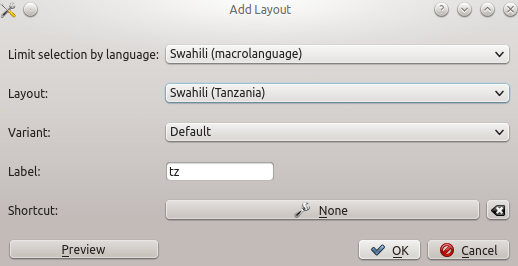
\includegraphics[keepaspectratio=true]{./images/kdelg.png}
% kdelg.png: 518x266 pixel, 96dpi, 13.70x7.04 cm, bb=0 0 388 199
\caption{Setting up the Swahili keyboard for KDE}
\label{fig:kdelg}
\end{figure}

Click \textbf{OK}, and then \textbf{Apply} to exit.

You should now see an additional marker in the system tray at the bottom right of your screen, which will be the abbreviation for the default language on your desktop.  For instance, if you have UK English as the default, you will see \textbf{gb}.  Click on this, and it will change to \textbf{tz}, showing that the keyboard for Swahili in Arabic script is now operational.  You can quickly switch between the two keyboards by pressing \textbf{Ctrl+Alt+K}.

Close the \textit{System Settings} box.

Note that if you make changes to the keyboard layout, you need to re-apply the layout -- see the end of \Cref{appC}.

\subsection{Activate the new keyboard in Unity}

If you have decided to stick to Unity as your desktop, click the \textbf{System Settings} icon in the Launcher, or click the system icon in the top right-hand corner and select \textbf{System Settings}.

Click \textbf{Text entry} in the \textit{Personal} section.

Click on the + at the bottom of the left-hand pane, \textit{Input sources to use}.

Roll down to \textit{Swahili (Tanzania)}.

Click on it and then click \textbf{Add}.

Close the \textit{Text entry} box.

There should be a new icon on the menu bar.  Either Click on the language chooser icon on the menu bar and choose Swahili from the list.  Alternatively, press \textbf{Super} (usually the key with a Windows logo on it) \textbf{+ Space}.

\subsection{Interaction with the unlock screen in KDE}

If you have the unlock screen activated, this means that when you leave your machine for some time, it will power down the screen and then, when you resume work, present a login box so that you can unlock the desktop.   A problem arises if you changed the  keyboard to Swahili before leaving your machine -- since the machine was powered down with that keyboard active, the login box will only allow you to type Arabic glyphs, which means that you cannot type in your (Roman glyph) password!

The easiest way to deal with this is to disable the unlock screen by going to \textbf{K} \textrightarrow\ \textbf{Settings} \textrightarrow\ \textbf{System Settings \textrightarrow\ Power Management \textrightarrow\ Advanced Settings}, and unticking \textit{Lock screen on resume}.

If for some reason you wish to retain the lock screen, you can recover from this situation whenever it occurs by pressing \textbf{Crtl+Alt+F5} to get a terminal login.  Type your username and password to log in.

Open the configuration file for the keyboard:\\
\verb|nano ~/.kde/share/config/kxkbrc|

Find the line:\\
\verb|LayoutList=gb,tz|\\
and change it to:\\
\verb|LayoutList=gb|

Save the file: \textbf{Ctrl+X, Y, Return}.\\
(The example here uses the UK English keyboard, \textit{gb} -- replace this with whatever your own default keyboard is.)

Press \textbf{Ctrl+Alt+F7} to return to the unlock screen.  Click the login box, and you should be able to login as normal.  However, you will need to re-add the Swahili keyboard as shown above.


\section{LibreOffice}
\label{s:libreoffice}

LibreOffice, installed by default in Ubuntu, is a suite of office software (word processor, spreadsheet, presentation program, etc).  The version used here is 4.2.4.2.

\subsection{Configure the word-processor}

Open LibreOffice Writer.

Click on \textbf{Tools \textrightarrow\ Options \textrightarrow\ Language Settings \textrightarrow\ Languages}.

Under \textit{Default languages for documents}, tick \textbf{Complex text layout (CTL)}, and select \textbf{Arabic (Oman)} in the dropdown.  Click OK.

Click on \textbf{Tools \textrightarrow\ Options \textrightarrow\ Language Settings \textrightarrow\ Complex Text Layout}.

If you wish to use both Arabic-Indic numerals (on the numeral keys) and Western-Arabic numerals (AltGr+numeral), ensure Arabic or System is chosen here. The other two settings will convert Western-Arabic numerals to their Arabic-Indic equivalents.

Tick \textbf{Visual} under \textit{Cursor control}, and then \textbf{OK}.

Right-click on the toolbar, and under \textit{Visible buttons} select \textbf{LTR}.  Do the same to select \textbf{RTL}.  Two new buttons will now appear in the Formatting toolbar, one for left-to-right typing, and one for right-to-left typing.

Shortcuts are \textbf{Ctrl+Shift+A} for LTR and \textbf{Ctrl+Shift+D} for RTL.

\subsection{Install a template}

Andika! includes in \textit{andika/libreoffice} a template (\textit{andika.ott}) where styles for Swahili in Arabic script, Swahili in Roman script (standard spelling or close transcription) and translation are already set up -- all these styles are right-justified.  Installing the template is optional, but it will make typing out Swahili poetry much simpler.

Click on \textbf{File \textrightarrow\ Templates \textrightarrow\ Manage}.

On the \textit{Documents} tab, double-click \textbf{My Templates} and then click \textbf{Import}.

Navigate to \textit{andika/libreoffice/andika.ott} and click on it -- it should now be listed there as a template.

If you want to set it as the default (nothing has been changed from the stock default apart from the addition of the three extra styles), click on it and then click \textbf{Set as default}.

To use the template without setting it as default, select \textbf{File \textrightarrow\ New \textrightarrow\ Templates \textrightarrow\ andika}.

Close the \textit{Templates} box, and then restart LibreOffice Writer.

To use the styles, place the cursor in the line you wish to format, press \textbf{F11} to open the \textit{Styles and Formatting} list, and select the relevant style by double-clicking on its name -- the new styles are at the bottom of the list.

\textit{Arabic} style is RTL, Scheherazade 24pt.  You may wish to make the font size smaller. In unvocalised Arabic, reading the text is possible at quite small font sizes. In Swahili, however, the vowel signs are essential, so the same reductions in font size are not possible.  In typesetting poetry, the lines are usually short, and accuracy is improved by having a large font size.

\textit{Roman} style is LTR, right-justified, Liberation Serif 12pt.

\textit{Translation} style is LTR, right-justified, Liberation Serif 12pt, italic.  

Obviously, the appropriate writing system (Arabic or Roman) also has to be selected on the keyboard before typing (see \Cref{s:keyboard}).


\section{PHP}

PHP is a computer language which is used to convert text from one script to the other, and also for the import and export of text to and from the database.

\subsection{Install PHP}

\verb|sudo apt-get install php5 php5-cli|

To test the install:\\
\verb|php --version|\\
(note: two dashes)\\
You should get a message giving details about the version of PHP you've just installed.

\subsection{Configure PHP}

\verb|sudo nano /etc/php5/cli/php.ini|

This command will open the system file \textit{php.ini} in a lightweight text editor called \textit{nano}, where you have to change some settings.  Use the arrow keys on the keyboard to move around, and the Home and End keys to move to the beginning or end of a line.

Press \textbf{Ctrl+W}, then type\\
\verb|max_execution_time|\\
into the searchline and press \textbf{Return}. Change the line to read:\\
\verb|max_execution_time = 300|

Again press \textbf{Ctrl+W}, type\\
\verb|error_reporting| \\
and press \textbf{Return}. Change that line to: \\
\verb|error_reporting = E_ALL & ~E_NOTICE & ~E_DEPRECATED|

A bit lower down from that (you can scroll down using the mouse), there is a \textit{display\_errors} line. Change it to read: \\
\verb|display_errors = On|

Below that there is a \textit{log\_errors} line. Change it to read: \\
\verb|log_errors = Off|

To save the file, press \textbf{Ctrl+X}, then press \textbf{Y} to confirm you want to save the modifications, and press \textbf{Return} to close the file.


\section{PostgreSQL}

PostgreSQL is a database which is used to store the words of the text for editing and enhancement.


\subsection{Install PostgreSQL}

\verb|sudo apt-get install postgresql postgresql-client postgresql-common|

$\hookrightarrow$ \verb|postgresql-contrib php5-pgsql|

To test the install:\\
\verb|psql|

You should get an error message saying that the role named after your username does not exist.


\subsection{Set up a database user}
\label{ss:dbuser}

On Ubuntu, PostgreSQL uses peer authentication by default.  This means that creating a database user with the same name as your system (Ubuntu) user will mean you can log in to the database without entering a password.\footnote{If for security reasons you wish to enter a password each time your user accesses a database, open the configuration file: \texttt{sudo nano /etc/postgresql/9.3/main/pg_hba.conf}.  Find the line: \texttt{local all all peer} and change it to read \texttt{local all all md5}.  Save the file: \textbf{Ctrl+X, Y, Return}.  Restart PostgreSQL: \texttt{sudo service postgresql restart}.  You will now need to enter your database password even to connect to the database under your system username.}  The terminal prompt should tell you what your username is -- it is of the form \textit{user@computer}.  Alternatively, you can run:\\
\verb|whoami|\\
to find out your username.

\verb|sudo -i|

The prompt will change to show that you are now \textit{root} (the superuser, or administrator).

\verb|su - postgres|\\
(note the space on either side of the dash)

The prompt will change to show that you are now the \textit{postgres} master user.

Create a new database user with the same name as your system user (replace USER with your system username):\\
\verb|createuser -P -s -e USER|

You will be asked to enter a password -- note that you will get no feedback (the line will stay blank).  Press \textbf{Return} and you will be asked to enter the password again.  Press \textbf{Return} and you should get a message beginning \textit{CREATE ROLE}, meaning that the new user has been created.

\verb|exit|\\
to cease being the postgres user.

\verb|exit|\\
to cease being the superuser.


\subsection{Set Andika! to use your database user}

\verb|nano andika/config.php|

Change:\\
\verb|user=kevin password=kevindbs|\\
to read:\\
\verb|user=USER password=yourpassword|\\
and save the file (\textbf{Ctrl+X, Y, Return}).

Remember to replace USER with your username.


\subsection{Create the andika database}

\verb|createdb andika|

This creates the \textit{andika} database, owned by your new user.

\textbf{Andika!} comes with starter data in \textit{andika/db/starter/andika.sql}, which can be imported into the new database:\\
\verb|psql -d andika < db/starter/andika.sql|

If you chose a username other than \textit{dbmaster}, use that instead.


\subsection{Connect to the \textit{andika} database}
\label{ss:connect}

\verb|psql -d andika|

The prompt should change to \textit{andika=\#}. 

\verb|\dt|\\
(= display tables)

This should show a list with 18 rows, each representing a database table holding poem information in the \textit{andika} database.  To look at the table for the poem \textit{kiswahili}:

\verb|select * from kiswahili;|\\
(note: the semicolon at the end is an integral part of the command)

This will show everything in the \textit{kiswahili} table.  Exit the data display and go back to psql:\\
\verb|q|

To see something more selective:\\
\verb|select * from kiswahili where stanza=1 order by stanza, loc;|\\
(again, remember the semicolon at the end)

You should get a listing of the \textit{vipande} in the first stanza of the poem \textit{Kiswahili} from the Abdulkadir and Frankl paper, in order of \textit{kipande}.  Exit the data display and go back to psql:\\
\verb|q|

\verb|\q|\\
to exit \textit{psql}.


\section{Database interfaces}

To make it easier to read and edit the contents of the PostgreSQL database, it is best to install an interface.  Two of these will be installed, each differing in their capabilities.  The first is a web-based interface called phpPgAdmin, which first requires a webserver (Apache) to be installed.  The second interface is called SQL Workbench, and it requires a computing language called Java to be installed.

\subsection{phpPgAdmin}

\subsubsection{Install Apache}
\label{ss:apache}

\verb|sudo apt-get install apache2 apache2-utils phppgadmin|

Start the webserver:\\
\verb|sudo service apache2 start|

If you want to get rid of the (harmless) message \textit{Could not reliably determine the server's fully qualified domain name, using 127.0.1.1. Set the `ServerName' directive globally to suppress this message}, issue the following commands:\\
\verb+echo "ServerName localhost" | sudo tee /etc/apache2/conf-available/servername.conf+\\
\verb|sudo a2enconf servername|\\
\verb|sudo service apache2 restart|

Test the install -- open a web browser (preferably Firefox) and type:\\
\verb|http://localhost|\\
into the address bar. A page should open, telling you that Apache is installed and working.

\subsubsection{Configure phpPgAdmin}

Activate the phpPgAdmin configuration file:\\
\verb|sudo cp /etc/apache2/conf.d/phppgadmin /etc/apache2/conf-enabled/phppgadmin.conf|

Restart the webserver:\\
\verb|sudo service apache2 restart|

In the web browser, type\\
\verb|http://localhost/phppgadmin|\\
into the address bar.

You should see the phpPgAdmin homepage. On the left side there is a list of servers (in this case, there should only be one listed). Click on \textbf{PostgreSQL} and you should get a login form.

Fill in the username and password for PostgreSQL (which you created in \Cref{ss:dbuser}) and click \textbf{Login}.

The default session time for PHP is set to 24 minutes (1440 seconds).  This means that if you do not use phpPgAdmin for 24 minutes, it will ask you to log in again before you can continue using it.  If you find that this interrupts your workflow, you can change the setting in the PHP configuration file:\\
\verb|sudo nano /etc/php5/apache2/php.ini|

Press \textbf{Ctrl+W}, then type:\\
\verb|session.gc_maxlifetime|

and press \textbf{Return}. Change the line to read: \\
\verb|session.gc_maxlifetime = 144000|

This will allow you 40 hours before logging you out, which should be sufficient.

\subsubsection{Test phpPgAdmin}
\label{ss:testppa}

In the left-hand panel you should get a list of your current databases -- there should only be two: \textit{andika} and the system database \textit{postgres}. (The right-hand panel shows you the same two databases.)

Click the \textbf{+} beside \textit{andika} in the left-hand panel.  It should open to show \textit{Schemas, public, Tables} etc. Click on \textbf{Tables}. The right-hand panel should now show you all the tables inside the \textit{andika} database, similar to what you saw in Section \ref{ss:connect}.

Click on \textbf{kiswahili} and you will see the data fields in that table. To see the contents of the database you can click on the \textbf{Browse} button.

To see the data fields of each item in more detail, click on the \textbf{Edit} button beside each row in the table -- changes to the fields can be made and saved here.

To make a database query, click the \textit{SQL} link at the top right of the phpPgAdmin window.  This will open another smaller window.  In the large textbox, type:\\
\verb|select * from kiswahili where stanza=1 order by stanza, loc;|\\
(again, remember the semicolon at the end)

Click Execute, and in the first window you should see a listing of the \textit{vipande} in the first stanza of the poem, in order of \textit{kipande}, as you did in Section \ref{ss:connect}.  In this case, though, the contents are a lot easier to read!


\subsection{SQL Workbench}
\label{ss:workbench}

\subsubsection{Install Java}

Andrei Alin\footnote{\url{webupd8.org}} maintains links to up-to-date versions of Java in his software repository.

Check that the helper script \textit{add-apt-repository} is installed:\\
\verb|sudo apt-get install software-properties-common|

Add the new software repository:\\
\verb|sudo add-apt-repository ppa:webupd8team/java|

Update the software package lists to include software from the new repository:\\
\verb|sudo apt-get update|

Install the Java installer:\\
\verb|sudo apt-get install oracle-java8-installer|

This installs a script that then downloads and installs Oracle Java 8 -- it may therefore take a few minutes.  To test the install:\\
\verb|java -version|\\
This should return some text telling you that the Java version is 1.8.0.

Set the Java environment variables:\\
\verb|sudo apt-get install oracle-java8-set-default|

\subsubsection{Install JDBC}
\label{ss:jdbc}

JDBC (Java DataBase Connector) is a driver which will allow SQL Workbench to connect to the PostgreSQL database.

\verb|sudo apt-get install libpostgresql-jdbc-java|

\subsubsection{Install SQL Workbench}

Create a directory to hold the files:\\
\verb|mkdir sqlworkbench|

Go to the website \textit{sql-workbench.net}, click on the link for \textit{Build 116} (or whatever the current stable version is), and download the generic package.  Save it in the \textit{andika} directory.

Unzip the download into the new directory:\\
\verb|unzip -q Workbench-Build116.zip -d sqlworkbench|

Make the launch script executable:\\
\verb|chmod +x sqlworkbench/sqlworkbench.sh|

Launch SQL Workbench:\\
\verb|sqlworkbench/sqlworkbench.sh|

If you wish, you can make a desktop shortcut or menu entry to make launching SQL Workbench easier.

\subsubsection{Configure SQL Workbench}

A \textit{Select Connection Profile} box should come up. 

Change \textit{New profile} to read \textbf{andika}.

Click the drop-down arrow on the \textit{Driver} line and select \textit{PostgreSQL}. Click \textbf{Yes}, when you're asked whether you want to edit the driver definition.

On the \textit{Manage Drivers} popup, click on the red \textit{postgresql} entry already there and then click X to delete it.  Click on the folder icon and navigate to \textit{/usr/share/java/postgresql-jdbc4-9.2.jar} (which you installed in Section \ref{ss:jdbc}.  Click \textbf{Open}, and then \textbf{OK}.

Check that the \textit{URL} line reads \textit{jdbc:postgresql://localhost:5432/andika} -- if not, edit it to make it so. Enter your PostgreSQL username and password (Section \ref{ss:dbuser}), and then click \textbf{OK}.  You should get a connecting message.

\subsubsection{Test SQL Workbench}

The main screen consists of a top pane where you type database queries, and a bottom pane where the results will appear. 

In the top pane, type:\\
\verb|select * from kiswahili where stanza=1 order by stanza, loc;|\\
(remember: the semicolon at the end is an integral part of the command)

Move the cursor somewhere in the middle of that query and press \textbf{Ctrl+Return}.  In the bottom pane, you should see a listing of the \textit{vipande} in the first stanza of the poem, in order of \textit{kipande}, as you did in Sections \ref{ss:connect} and \ref{ss:testppa}.

The main benefit of SQL Workbench compared to phpPgAdmin is that a result set can be directly edited -- this makes it easy to add data.  To try this, select one of the cells under the \textit{english} column, type something in, and press \textbf{Return}.  A yellow diamond will appear in the leftmost column, showing that the record has been edited but not saved yet. To save it you need to click the disk icon, or select \textbf{Data \textrightarrow\ Save changes to database} and click \textbf{OK} when asked to confirm.

You can check the change was made by running the same query in phpPgAdmin's SQL box (see Section \ref{ss:testppa}) :\\
\verb|select * from kiswahili where stanza=1 order by stanza, loc;|

To delete the change, click the cell in SQL Workbench, press \textbf{Backspace} and then \textbf{Return}, and then save as before.

Close SQL Workbench, clicking Yes to save the new \textit{andika} connection profile you have set up.


\section{LaTeX}
\label{s:latex}

LaTeX is a typesetting system that is capable of creating very complex layouts.  It is used in \textbf{Andika!} to provide attractive output.

\verb|sudo apt-get install texlive texlive-xetex texlive-generic-extra texlive-humanities|\\
$\hookrightarrow$ \verb|texlive-lang-arabic texlive-latex-extra texlive-bibtex-extra kile kbibtex biber|

Note that these packages will take perhaps 20 minutes to download and install.


\section{JabRef}
\label{s:jabref}

JabRef\footnote{jabref.org} is a bibliography manager.

\verb|sudo apt-get install jabref|


\section{YAD}

YAD (Yet Another Dialogue),\footnote{\url{sourceforge.net/projects/yad-dialog/}} maintained by Victor Ananjevsky, is used by \textbf{Andika!} to provide a point-and-click interface to the conversion script.  To install it, we need to add another of Andrei Alin's\footnote{\url{webupd8.org}} repositories.

Add the new software repository:\\
\verb|sudo add-apt-repository ppa:webupd8team/y-ppa-manager|

Update the software package lists to include software from the new repository:\\
\verb|sudo apt-get update|

Install YAD:\\
\verb|sudo apt-get install yad|\footnote{You may also wish to install Andrei's own Y-PPA-Manager -- \texttt{sudo apt-get install y-ppa-manager}.  This is not used by \textbf{Andika!}, but is a very useful system tool to keep track of the software repositories on your machine.}


\section{Access the \textit{Andika!} website locally}
\label{s:localaccess}

Although not essential to use \textbf{Andika!}, it may be useful to have access to a local copy of the website (\textit{kevindonnelly.org.uk/swahili}).  

First, tell the webserver installed earlier (Apache -- see Section \ref{ss:apache}) where to find the\textbf{ Andika!} webpages.

Open a configuration file:\\
\verb|sudo nano /etc/apache2/sites-available/andika.conf|

Type the following lines into the file:\\
\vspace{-0.5cm}  % get rid of the excess space before the verbatim environment
\begin{verbatim}
<VirtualHost *:80>
ServerName andika
DocumentRoot /var/www/andika/
</VirtualHost>
\end{verbatim}

Save and exit the configuration file:\\
\textbf{Ctrl+X, Y, Return}

Activate the configuration:\\
\verb|sudo a2ensite andika|

Restart the webserver:\\
\verb|sudo service apache2 restart|

Then tell your web browser that the new website is on your machine, so it doesn't have to look for it on the web.

Open a configuration file:\\
\verb|sudo nano /etc/hosts|

After the line:\\
\verb|127.0.0.1	localhost|\\
add the following line:\\
\verb|127.0.0.1	andika|

Save and exit the configuration file:\\
\textbf{Ctrl+X, Y, Return}

In a web browser, type:\\
\verb|http://andika/index.php|\\
into the address bar.  You should get the \textbf{Andika!} website loading from the files on your hard disk (in \textit{/var/www/andika}), instead of from the internet.



% stackoverflow.com/questions/1209065/to-have-no-pagebreak-after-include-in-latex


\newpage


%----------------
% Appendix B: adding missing glyphs 
%----------------
\chapter{Editing fonts}
\renewcommand{\thesection}{B/\arabic{section}}  % redefine the section numbering
\setcounter{section}{0}  % reset counter
\label{appB}

\begin{quotation}
\noindent I am grateful to Khaled Hosny\footnote{\url{khaledhosny.org}} for his advice on using FontForge to edit Arabic glyphs, which has been incorporated in these instructions.
\end{quotation}

\section{Introduction}
\label{appb:intro}

Most Arabic fonts are missing some glyphs that are essential to allow them to be used for writing Swahili.  This appendix deals with how to edit these fonts to add the missing glyphs.  This will entail editing the font with FontForge\footnote{\url{fontforge.github.io/en-US}} (originally developed by George Williams).

\section{Install FontForge}

There are two options here -- the easiest is to use a pre-compiled package.

\subsection{Use a pre-compiled package}

The FontForge package included in Ubuntu 14.04 by default dates from 2012, so it is preferable to install the more up-to-date package from the FontForge Personal Package Archive (PPA).\footnote{\url{https://launchpad.net/~fontforge/+archive/ubuntu/fontforge}}

Check that the helper script add-apt-repository is installed:

\verb|sudo apt-get install software-properties-common|

Add the FontForge PPA (which will also add the authentication key):

\verb|sudo add-apt-repository ppa:fontforge/fontforge|

Update the package list:

\verb|sudo apt-get update|

Install FontForge:

\verb|sudo apt-get install fontforge|


\subsection{Compile from the source code}

In some cases, perhaps because you want access to a feature not yet available in the pre-compiled package, you may wish to compile your own version from the code available on GitHub.\footnote{\url{github.com/fontforge/fontforge}}

\subsubsection{Install preliminary software}

Install packages to allow the building of software:

\verb|sudo apt-get install build-essential automake flex bison|

Install the \textit{unifont} package to get a full display of the reference glyphs.  Unifont\footnote{\url{savannah.gnu.org/projects/unifont}} includes glyphs for all Unicode codepoints, and FontForge will use it if it is installed.

\verb|sudo apt-get install unifont|

Install other required packages: 

\verb|sudo apt-get install packaging-dev pkg-config python-dev libpango1.0-dev|\\
$\hookrightarrow$ \verb|libglib2.0-dev libxml2-dev giflib-dbg libjpeg-dev libtiff-dev uthash-dev|

\subsubsection{Build \textit{libspiro}}

FontForge uses \textit{libspiro}\footnote{\url{github.com/fontforge/libspiro}} (by Raph Levien) to simplify the drawing of curves.

Download the code:

\verb|git clone https://github.com/fontforge/libspiro.git|

Run the following commands in sequence (that is, wait for each one to complete before running the next):
\begin{verbatim}
cd libspiro
autoreconf -i
automake --foreign -Wall
./configure
make
sudo make install
cd ..
\end{verbatim}

\subsubsection{Build \textit{libuninameslist}}

FontForge uses \textit{libuinameslist}\footnote{\url{github.com/fontforge/libuninameslist}} to access attribute data about each Unicode code point.

Download the code:

\verb|git clone https://github.com/fontforge/libuninameslist.git|

Run the following commands in sequence (that is, wait for each one to complete before running the next):
\begin{verbatim}
cd libuninameslist
autoreconf -i
automake --foreign
./configure
make
sudo make install
cd ..
\end{verbatim}

\subsubsection{Build FontForge}

Download the code:

\verb|git clone https://github.com/fontforge/fontforge.git|

Run the following commands in sequence (that is, wait for each one to complete before running the next):
\begin{verbatim}
cd fontforge
./bootstrap
./configure
make
sudo make install
cd ..
\end{verbatim}

Make the system aware of the new libraries:

\verb|sudo ldconfig|


\section{Make a working copy of the font}

The font we will add glyphs to is Graph\footnote{\url{openfontlibrary.org/en/font/graph}} (regenerated by Nadim Shaikli).  A version of the following howto which includes images is available on the \textit{Design with FontForge} website.\footnote{\url{http://designwithfontforge.com/en-US/Adding_Glyphs_to_an_Arabic_Font.html}}

Download the font from the webpage into the \textit{andika} directory.  Unzip it, and delete the zip file:

\verb|unzip -q graph.zip -d fonts && rm graph.zip|

Launch FontForge (in KDE, go to \textbf{K \textrightarrow\ Graphics \textrightarrow\ FontForge}).  Note that FontForge is built using the programming language Tcl,\footnote{\url{tcl.tk/}} and it therefore behaves slightly differently from other software you may be used to.  For instance, every action requires at least one click (so the submenus for menus don't appear as you move across the menu bar -- you have to click each one).

The first time you open FontForge, it will ask to you load a font.  Navigate to \textit{andika/fonts}, select \textit{ae\_Graph.ttf}, and click \textbf{OK}.  FontForge will display a chart of every glyph in the font, each in its own cell.  The smaller cell above it is a reference glyph -- not all reference glyphs will have a font glyph, since few fonts contain glyphs for every single Unicode code point.  Where the font glyph is missing, the cell will contain a grey X.

Save it as an sfd file which will become your working copy: select \textbf{File \textrightarrow\ Save}, edit the suggested name to read \textbf{GraphSwa.sfd} and click \textbf{Save}.

\section{Rename the font}

If you do not rename the font, your adapted font will not install separately from the original -- you will have to uninstall the original font first.  It is also sensible to rename the font if you are going to distribute your adaptations -- if the original author of the font has reserved the font name under the Reserved Font Name (RFN) mechanism, that original name can only be used with the original author's version of the font.

If you adapt a font that was originally under an open license (eg GPL\footnote{\url{gnu.org/copyleft/gpl.html}} or OFL\footnote{\url{scripts.sil.org/OFL-FAQ_web}}) and then distribute it, you must retain the original author's copyright notices and licensing information, although you can append a note at the end of the copyright notice covering your contribution.

Note that adapting a font that was originally under a closed license (eg most fonts by Microsoft, Adobe, Bitstream, Linotype, etc), may be a breach of copyright, depending on the terms of the license.

Select \textbf{Element \textrightarrow\ Font Info}, and in the \textit{PS Names} panel, change \textit{Fontname}, \textit{Family Name}, and \textit{Name For Humans} to \textbf{GraphSwa}.

In the \textit{TTF Names} panel, the names for \textit{Family} and \textit{Fullname} are taken from the \textit{PS Names} entries, and should already be showing \textit{GraphSwa} (you can't edit them directly).  Change the entries for \textit{Preferred Family} and \textit{Compatible Full} to \textbf{GraphSwa}.  These name changes will now allow you to install this font alongside the original one if you wish.

If desired, in the \textit{TTF Names} panel you can also place a "Swahili glyphs added by" message after the text already in the entry for \textit{Designer}.

Click \textbf{OK} to save these changes.  You will get a message about generating a new UniqueID (XUID) for the font -- click \textbf{Change}.

\section{Add the glyph for the isolated form of \textit{peh}}
\label{s:pehisol}

We will add the missing glyph \textit{peh} (U+067E) to the Graph font.

Go to the Arabic section of the font chart: select \textbf{View \textrightarrow\ Go to}, click the dropdown box and select \textbf{Arabic}, then click \textbf{OK}.

Clicking on a cell in the font chart will show its Unicode number and name in blue at the top of the panel.  Go to position \textit{1662 (0x67e) U+067E ``uni067E'' ARABIC LETTER PEH}.  The cell below the reference glyph contains a grey X, showing that the font does not include this glyph.

We will make \textit{peh} by copying \textit{beh} (U+0628) and swapping its single dot for three dots.

Click on the \textit{beh} cell (position 1576), then right-click and select \textbf{Copy}.  Then right-click on the \textit{peh} cell and select \textbf{Paste}.  Now that \textit{beh} is now copied into the \textit{peh} cell, the next thing is to change the dot.

Find a glyph with three dots -- \textit{sheen} (position 1588, U+0634) will do.  Double-click on the cell -- this will open a glyph design panel.  Press \textbf{V} to ensure the pointer tool (arrowhead) in the toolbox is selected, and press \textbf{Z} and enlarge the panel to give you a good view of the glyph.

Click and drag so that the nodes of the three dots above sheen change colour from pink to beige.  If you accidentally include or omit a node, deselect or select it by pressing \textbf{Shift} and clicking.  Press \textbf{Alt+C} to copy.

Go back to the font chart and double-click on the \textit{peh} cell -- this will load \textit{peh} into another tab in the glyph design panel, alongside the \textit{sheen} tab.

Click and drag to highlight the dot below \textit{peh}, then press \textbf{Delete}.  Press \textbf{Alt+V} to paste in the three dots, which will likely appear above the body of \textit{peh}.  Leave the dot nodes highlighted so that you can invert and move them more easily.

Invert the dots: select the flip tool (two triangles with a red dashed line between them) from the toolbox.  (Alternatively, right-click in the middle of the dots, and select \textbf{Flip the selection} from the popup.)  Click on one of the dot nodes and drag the mouse slightly left or right.

Move the inverted dots: press \textbf{V} to select the pointer tool again, click on one of the dot nodes, and drag them down below the body of the glyph.  Position them centrally, above the \textit{ArabicBelow} mark.

Close the glyph design panel. There should now be a new glyph for \textit{peh} in the font chart.  Save the adapted font (\textbf{File \textrightarrow\ Save}).


\section{Add the glyphs for the connected forms of \textit{peh}}

However, this is only the isolated (standalone) form of the glyph.  If you try to use your adapted font, you will find that initial, medial and final forms are not available.  These have to be created separately.  "The[se] forms are built as unencoded glyphs (glyphs whose encoding is -1 in FontForge conventions).  Th[ey] have no predefined slots." (Khaled Hosny)

Select \textbf{Encoding \textrightarrow\ Add Encoding Slots} and enter the number of the glyphs you want -- in this case \textbf{3}.  FontForge will add the same number of slots at the very end of the font, and you will be moved there in the font chart.  The last three cells (positions 65537, 65538, 65539) have a question mark as a reference glyph, and it is in those cells that you will add the unencoded glyphs by repeating the process in \Cref{s:pehisol} above.

Note that if by mistake you start typing when the font chart still has focus, you get moved to the European section at the top.  To get back to the bottom, select \textbf{View \textrightarrow\ Go to}, click the dropdown box and select \textbf{Not a Unicode Character},  and then click \textbf{OK}.

\subsection{Create the final form}

Roll the font chart up a bit until you come to a set of Arabic glyphs at position 65152 (U+FE80) onwards.  At U+FE90 (position 65168) you will see a \textit{behfinal} glyph -- click on it and press \textbf{Ctrl+C} to copy it.  Roll down to the third last cell in the chart (position 65537), click on it, and press \textbf{Ctrl-V} to paste in the \textit{behfinal} glyph.

Right-click on the cell and select \textbf{Glyph Info}.  The naming convention is to use the number of the isolated glyph + a suffix for the form, so change \textit{Glyph Name} to \textbf{uni067E.fina},  and click \textbf{OK}.  The question mark in the reference cell will change to \textit{peh}.

Get the three dots: double-click on \textit{sheen} (U+FEB5) to load it into the glyph design panel, select the three dots and press \textbf{Ctrl+C}.

Double-click on the new \textit{pehfinal} to load it into the glyph design panel, click and drag to highlight the nodes of the dot and press \textbf{Delete}.

Ctrl+V to insert the three dots from \textit{sheen}, flip them, and move them into position below the glyph body.  Press \textbf{Ctrl+S} to save the revised font chart.

\subsection{Create the initial and medial forms}

Copy the initial form U+FE91 (position 65169) to the penultimate cell (position 65538), delete the single dot and paste in the three dots.

Right-click the cell, select \textbf{Glyph Info}, change \textit{Glyph Name} to \textbf{uni067E.init}, and click \textbf{OK}.

Copy the medial form U+FE92 (position 65170) to the last cell (position 65539), delete the single dot and paste in the three dots.

Right-click the cell, select \textbf{Glyph Info}, change \textit{Glyph Name} to \textbf{uni067E.medi}, and click \textbf{OK}.

Select \textbf{File \textrightarrow\ Save} to save the revised font chart.

\subsection{Add the lookups}

The isolated form has to be mapped (linked) to its initial, medial and final forms.

Select \textbf{Element \textrightarrow\ Font Info \textrightarrow\ Lookups}.

Click on the \textbf{+} beside the entry \textit{'init' Initial Forms in Arabic lookup 2}.  This will open a submenu of the same name.  Click on this submenu.

The \textit{Edit Data} button on the right will now become available -- click it.

In the \textit{Lookup Subtable} panel that pops up, ensure that the \textit{Unicode} button is checked.  Roll the list of characters down until you come to the end.

In the box beside \textit{Default Using Suffix}, enter the relevant suffix (in this case, \textbf{init}), and then click \textbf{Default Using Suffix}.

A new mapping will be added to the list of characters, from uni067E (the isolated form of \textit{peh}) to uni067E.init (the initial form).
Click \textbf{OK}.

Do the same for the submenus under the entries \textit{'medi' Medial Forms in Arabic lookup 2} and \textit{'fina' Terminal Forms in Arabic lookup 2}, choosing \textit{medi} and \textit{fina} as the relevant suffix.

Click \textbf{OK} again to close the panel, and save the font chart (\textbf{Ctrl+S}).

Note that \textit{Default Using Suffix} only seems to work on glyphs in the Unicode 06 (\textit{Arabic}) block -- glyphs in Unicode 07 (\textit{Arabic Supplement}), eg \textit{ain} with two dots, may have to be added manually by clicking the line marked \textit{New} and typing in the names.

\section{Generate the adapted font}

Select \textbf{File \textrightarrow\ Generate Fonts}.

In the dropdown showing \textit{PS Type 1 (Binary)}, select \textbf{TrueType}, and check that the filename reads \textit{GraphSwa.ttf}.

Navigate to where you want to save the font, and then click \textbf{Generate}.  Click \textbf{Yes} and \textbf{Generate} to the two information messages that come up.  You can then use your normal font installation procedure (in KDE, \textbf{K \textrightarrow\ System \textrightarrow\ System Settings \textrightarrow\ Font Management}) to install the adapted font.

\section{Next steps}

You will need to carry out the above process to add all the missing glyphs listed in \Cref{tab:missglyphs}.

Note that if you make changes to a font, you need to restart LibreOffice in order to use the changed font, because it will see only the previous version of the font, and not the new changes.



\newpage



%----------------
% Appendix C: editing the keyboard
%----------------
\chapter{Changing the \textbf{Andika!} keyboard layout}
\renewcommand{\thesection}{C/\arabic{section}}  % redefine the section numbering
\setcounter{section}{0}  % reset counter 
\label{appC}

\section{Introduction}

The layout of the \textbf{Andika!} keyboard is specified in the file \textit{layout/tz}.  The file (reproduced in \Cref{appE}) is a simple text file, and can be easily adapted to add new glyphs or change the position of existing glyphs.

Each line follows the pattern below:

\verb|key <AC03> { [Arabic_dal, Arabic_thal, Arabic_dad, Arabic_ddal] };|

The key number (in this case AC03, for the \textbf{D} key) is followed by a sequence of 4 glyph names (in this case representing \AS{ڈ ض ذ د}).  The sequence specifies the glyph that will be output when (respectively) the user presses \textbf{D}, \textbf{Shift+D}, \textbf{AltGr+D}, and \textbf{AltGr+Shift+D}.

Some lines have less than four entries.  For instance, the \textbf{P} key only has one entry (\AS{پ}):

\verb|key <AD10> { [Arabic_peh] };|

because that is the only glyph output by that key, and the \textbf{S} key only has three entries ( \AS{ص ش س}):

\verb|key <AC02> { [Arabic_seen, Arabic_sheen, Arabic_sad] }|

giving the glyphs that will be output by pressing \textbf{S}, \textbf{Shift+S} and \textbf{AltGr+S}.

If it is desired to block one of the slots, to enforce a particular keypress for a glyph, the entry \verb|NoSymbol| can be used.  Thus in the line for the \textbf{5} key:

\verb|key <AE05> { [Arabic_5, NoSymbol, KP_5, percent] };|

the output will be \AS{٥} for \textbf{5}, nothing for \textbf{Shift+5}, Western 5 for \textbf{AltGr+5} and a percent sign for \textbf{AltGr+Shift+5}.  Without the \verb|NoSymbol|, the output would be \AS{٥} for \textbf{5}, Western 5 for \textbf{Shift+5}, a percent sign for \textbf{AltGr+5} and nothing for \textbf{AltGr+Shift+5}.

Glyph names are available for some, but by no means all, of the possible glyphs.\footnote{\url{http://wiki.linuxquestions.org/wiki/List_of_Keysyms_Recognised_by_Xmodmap}}  Where no name is available, the Unicode codepoint can be used instead.  Thus, in the line for the \textbf{n} key:

\verb|key <AB06> { [Arabic_noon, U075D] };|

\AS{ن} will be output when the \textbf{N} key is pressed, and the glyph represented by Unicode 075D (\AS{ݝ}, \textit{ain} with two dots above) will be output when \textbf{Shift+N} is pressed.  It would be possible to use nothing but Unicode codepoints in the file, but using the glyph names makes it a bit easier to read.

From the above, it will be obvious that adjusting the location of a particular glyph merely consists of moving it to the desired slot on the desired key.  For example, if the user wanted \AS{ض} to appear when Shift+D is pressed, and \AS{ذ} when AltGr+D is pressed, all that needs to be done is to open the file:

\verb|sudo nano layout/tz|

and change the line:

\verb|key <AC03> { [Arabic_dal, Arabic_thal, Arabic_dad, Arabic_ddal] };|

to:

\verb|key <AC03> { [Arabic_dal, Arabic_dad, Arabic_thal, Arabic_ddal] };|

Then save the file by pressing \textbf{Ctrl+X}, \textbf{Y}, and \textbf{Return}.

Likewise, adding a new glyph to the keyboard is as simple as deciding which slot on which key it should occupy, and then inserting the Unicode codepoint (or the glyph name where one exists) at that slot.  For instance, if the user needs to access the glyph \textit{rreh} (\textit{ra} with \textit{tah} as a diacritic, Unicode 0691), and decides to put it on the \textbf{R} key so that it will be output when \textbf{AltGr+R} is pressed, all that needs to be done is to change the line:

\verb|key <AD04> { [Arabic_ra] };|

to:

\verb|key <AD04> { [Arabic_ra, NoSymbol, U0691] };|

(Remember that if \verb|NoSymbol| is omitted here, \textit{rreh} will appear when \textbf{Shift+R} is pressed.)

In either case, the new layout has to be activated.  So, after saving the file, copy it to the correct location:

\verb|sudo cp layout/tz /usr/share/X11/xkb/symbols/|

Delete the cache files relating to the old layout (new ones will be created when the new layout is activated):

\verb|sudo rm /var/lib/xkb/server-*|

Then remove the \textit{tz} keyboard layout using your desktop's language setup utility and re-add it.  For KDE, this simply means going to \textbf{K} \textrightarrow\ \textbf{Settings} \textrightarrow\ \textbf{System Settings} \textrightarrow\ \textbf{Input Devices} \textrightarrow\ \textbf{Keyboard} \textrightarrow\ \textit{Layouts} tab, unticking \textbf{Configure layouts}, clicking \textbf{Apply}, and then reticking \textbf{Configure layouts} and clicking \textbf{Apply} again.

The new layout should then be ready for use.






\newpage


%----------------
% Appendix D: Kiswahili poem
%----------------
\chapter{Annotated poem, \AS{كِسْوَاحِلِ} (\textit{Kiswahili})}
\renewcommand{\thesection}{D/\arabic{section}}  % redefine the section numbering
\setcounter{section}{0}  % reset counter 

\citet{Abdulkadir2013} presents an annotated edition of the poem \AS{كِسْوَاحِلِ} by Mahmoud Ahmad Abdulkadir (Ustadh Mau).  The following is a letter-for-letter transcription of the author's manuscript as reproduced there, with the exception that the damma-with-tail occasionally used by him to signify \textbf{o} is denoted here with inverted damma (eg in \AS{كُوَأٗنَ نَ تَمَانِ} in 1d), since the font does not yet include that glyph.  The layout also includes automatically-generated close and standard transliterations, and the English translation and notes from that paper.  The document was generated automatically from a database table which held all the data about the poem (words, translation, notes, etc) -- see the \textit{kiswahili} table in the \textit{andika} database included in the \textbf{Andika!} download.

\begin{longtable}{rrl} 
\makebox[8cm][r]{} & & \makebox[8cm][r]{} \\ 

& \Atitle{كِسْوَاحِلِ} & \\*
& \S{Kiswahili} & \\*
& \E{Mahmoud Ahmad Abdulkadir} & \\

\\
\cline{1-2}[1pt/3pt] \\
\\
& \textarabic{بسم الله الرحمن الرهيم} & \\*
& \Tr{bismi llähi arraḥmani arraḥı̄mi} & \\*
& \S{bismillahi arrahmani arrahimi} & \\
\\

\textarabic{تَانْيَامَا حَتَ لِنِ} & \textarabic{كُنْيَمَا نِ مٖػوْكَ} & \textarabic{١} \\* 
\Tr{ṯānyāmā ḥaṯa lini} & \Tr{kunyamā ni mekʲūka} & \\* 
\multicolumn{2}{r}{\S{kunyamaa nimechoka * t'anyamaa hata lini}} & \S{1a/b} \\* 
\multicolumn{2}{r}{\E{I am weary of staying silent. For how much longer am I to remain dumb?}} & \\[2mm] 
\textarabic{كُوَأٗنَ نَ تَمَانِ} & \textarabic{وَنَنْڠُ هُنِئٖپُوْكَ} &  \\* 
\Tr{kuwaona na ṯamāni} & \Tr{wanangu huniepūka} & \\* 
\multicolumn{2}{r}{\S{wanangu huniepuka * kuwaona natamani}} & \S{1c/d} \\* 
\multicolumn{2}{r}{\E{My own children avoid me, though I long to see them.}} & \\[2mm] 
\textarabic{سِوَنْڠُ نِ وَ وٖنْدَانِ} & \textarabic{والُوْبَاكِ كُنِشِكَ} &  \\* 
\Tr{siwangu ni wa wenḏāni} & \Tr{wālūbāki kunishika} & \\* 
\multicolumn{2}{r}{\S{walobaki kunishika * si wangu ni wa wendani}} & \S{1e/f} \\* 
\multicolumn{2}{r}{\E{And those who remain to embrace me are not my own, but are the offspring of others.}} & \\[2mm] 
\textarabic{مْبُوْنَ هُنِپِجَ زِتَ} & \textarabic{مِمِ نِ مٖوَتٖنْدَانِ} &  \\* 
\Tr{mbūna hunipija ziṯa} & \Tr{mimi ni mewaṯenḏāni} & \\* 
\multicolumn{2}{r}{\S{mimi nimewatendani * mbona hunipija zita}} & \S{1g/h} \\* 
\multicolumn{2}{r}{\E{What have I done to you? Why do you wage war on me?}} & \\[2mm] 
\\[8mm] 

\textarabic{وَانَ وَ أُسْوَاحِلِنِ} & \textarabic{وَنَانْڠُ مِمِ وَ دَمُ} & \textarabic{٢} \\* 
\Tr{wāna wa uswāḥilini} & \Tr{wanāngu mimi wa ḏamu} & \\* 
\multicolumn{2}{r}{\S{wanangu mimi wa damu * wana wa Uswahilini}} & \S{2a/b} \\* 
\multicolumn{2}{r}{\E{My own flesh and blood, the children of Swahililand,}} & \\[2mm] 
\textarabic{يَا كُنِيُوَ نِ نَانِ} & \textarabic{أَصِلِ هَوَنَ هَامُ} &  \\* 
\Tr{yā kuniyuwa ni nāni} & \Tr{aṣili hawana hāmu} & \\* 
\multicolumn{2}{r}{\S{asili hawana hamu * ya kuniyuwa ni nani}} & \S{2c/d} \\* 
\multicolumn{2}{r}{\E{are uninterested in knowing who I am,}} & \\[2mm] 
\textarabic{نَ وَنَ وَ مَجِرَنِ} & \textarabic{وَمٖنَتِيَ قَؤُمُ} &  \\* 
\Tr{na wana wa majirani} & \Tr{wamenaṯiya qaumu} & \\* 
\multicolumn{2}{r}{\S{wamenatiya kaumu * na wana wa majirani}} & \S{2e/f} \\* 
\multicolumn{2}{r}{\E{and have left me to other peoples, and to the children of neighbours.}} & \\[2mm] 
\textarabic{مْبُوْنَ هُنِپِجَ زِتَ} & \textarabic{كُوْسَ لَنْڠُ كُوْسَ ڠَانِ} &  \\* 
\Tr{mbūna hunipija ziṯa} & \Tr{kūsa langu kūsa gāni} & \\* 
\multicolumn{2}{r}{\S{kosa langu kosa gani * mbona hunipija zita}} & \S{2g/h} \\* 
\multicolumn{2}{r}{\E{What kind of fault is my fault? [O my children] why do you continue waging war on me?}} & \\[2mm] 
\\[8mm] 

\textarabic{وَلَ سِنَ پُنْڠُوَنِ} & \textarabic{مِمِ مَامٖنُ سِتَاسَ} & \textarabic{٣} \\* 
\Tr{wala sina punguwani} & \Tr{mimi māmenu siṯāsa} & \\* 
\multicolumn{2}{r}{\S{mimi mamenu sit'asa * wala sina punguwani}} & \S{3a/b} \\* 
\multicolumn{2}{r}{\E{I am your mother and am not yet infertile, nor has my ability to reproduce diminished.}} & \\[2mm] 
\textarabic{نَ كُنْڠِنٖ زِسِوَنِ} & \textarabic{نِ مٖزَا وَ مَمْبَاسَ} &  \\* 
\Tr{na kungine zisiwani} & \Tr{ni mezā wa mambāsa} & \\* 
\multicolumn{2}{r}{\S{nimezaa wa Mambasa * na kungine zisiwani}} & \S{3c/d} \\* 
\multicolumn{2}{r}{\E{I have given birth to children in Mambasa, and in the other islands [of the Swahili],}} & \\[2mm] 
\textarabic{نَ زِيُوْنْڠُوْزِ وَدِنِ} & \textarabic{نِزٖ وَنَ سِيَاسَ} &  \\* 
\Tr{na ziyūngūzi waḏini} & \Tr{nize wana siyāsa} & \\* 
\multicolumn{2}{r}{\S{nizee wanasiyasa * na ziongozi wa dini}} & \S{3e/f} \\* 
\multicolumn{2}{r}{\E{to politicians and to religious leaders,}} & \\[2mm] 
\textarabic{نَ مَاشُجَا وَ زِتَ} & \textarabic{مَافُنْدِ وَ كُلَ فَنِ} &  \\* 
\Tr{na māshujā wa ziṯa} & \Tr{māfunḏi wa kula fani} & \\* 
\multicolumn{2}{r}{\S{mafundi wa kila fani * na mashujaa wa zita}} & \S{3g/h} \\* 
\multicolumn{2}{r}{\E{to craftsmen in every field, and to war heroes.}} & \\[2mm] 
\\[8mm] 

\textarabic{پِيَ مْوٖنْڠٗ عَثْمَانِ} & \textarabic{نْدِمِ مَامَاكٖ مُيَاكَ} & \textarabic{٤} \\* 
\Tr{piya mwengo 'ath}\I{u}\Tr{māni} & \Tr{nḏimi māmāke muyāka} & \\* 
\multicolumn{2}{r}{\S{ndimi mamake Muyaka\footnote{Bwana Muyaka was the outstanding Swahili poet of 19th century Mombasa.  After his death many of his verses were recalled by Mu'allim Sikujua Abdallah al-Batawi (died 1890) and transcribed with annotations by W.E. Taylor (1856-1927). After Taylor’s death his papers were acquired by the library of the School of Oriental and African Studies (SOAS), London.} * pia Mwengo Athumani\footnote{Mwengo Athmani: this 18th century poet from Pate composed the {\FN{Utendi wa Tambuka}} (\textit{The Epic of Heraklios}).}}} & \S{4a/b} \\* 
\multicolumn{2}{r}{\E{I am the mother of Bwana Muyaka, and of Mwengo Athmani also,}} & \\[2mm] 
\textarabic{نَ وٖنْڠِ وَاكٖ وٖنْدَانِ} & \textarabic{نَ زَهِدِ كَذَلِكَ} &  \\* 
\Tr{na wengi wāke wenḏāni} & \Tr{na zahiḏi kadhalika} & \\* 
\multicolumn{2}{r}{\S{na Zahidi\footnote{Zahidi: see El-Maawy (2008).} kadhalika * na wengi wake wendani}} & \S{4c/d} \\* 
\multicolumn{2}{r}{\E{and of Zahidi too, and many of his contemporaries,}} & \\[2mm] 
\textarabic{وٗتٖ مْبوَا مُوْيَ قَرِنِ} & \textarabic{عالى كُوْتِ نَ مَتَاكَ} &  \\* 
\Tr{woṯe mbwā mūya qarini} & \Tr{'ālı̄ kūṯi na maṯāka} & \\* 
\multicolumn{2}{r}{\S{Ali Koti\footnote{Ali Koti of Pate: see Chiraghdin (1987: 31-7).} na Mataka\footnote{Bwana Mataka’s full name is Muhammad bin Shee Mataka al-Famau (1825-1868). He was ruler of Siyu, as was his father. His mother was Mwana Kupona, famous for the poem of advice written to her daughter. Bwana Mataka died in Mombasa’s fort while imprisoned by the Busa‘idi.
} * wote mbwa moya karini}} & \S{4e/f} \\* 
\multicolumn{2}{r}{\E{Ali Koti and Mataka, all from just one century,}} & \\[2mm] 
\textarabic{وَ كَوَا كَمَ نْيوتَ} & \textarabic{وَلِتُوْكَ مَاتُوْمبونِ} &  \\* 
\Tr{wa kawā kama nı̄ūṯa} & \Tr{waliṯūka māṯūmbūni} & \\* 
\multicolumn{2}{r}{\S{walitoka matumboni * wakawaa kama nyota}} & \S{4g/h} \\* 
\multicolumn{2}{r}{\E{they emerged from my womb, and shone like stars.}} & \\[2mm] 
\\[8mm] 

\textarabic{أُكِسٗوْمٖ نَ كِدَنِ} & \textarabic{اِنْكِشَافِ نْڠَلِيَ} & \textarabic{٥} \\* 
\Tr{ukisōme na kiḏani} & \Tr{inkishāfi ngaliya} & \\* 
\multicolumn{2}{r}{\S{Inkishafi\footnote{The {\FN{Inkishafi}}, according to W.E. Taylor Stigand (1915: 96-105) is ``a great, if not the greatest, religious classic of [the Swahili-speaking peoples]''. The poem, concerned with the decay of Pate (formerly a flourishing town in northern Swahililand), may remind some readers of Thomas Gray's \textit{Elegy written in an English churchyard} (London 1751).
} angaliya * ukisome na kidani}} & \S{5a/b} \\* 
\multicolumn{2}{r}{\E{Look at Inkishafi. Read it attentively}} & \\[2mm] 
\textarabic{نِ كْوَامْبِيَاءٗ مْوٖنْدانِ} & \textarabic{نْدِپُوْ تَاكَاپُوْ كْوٖلٖيَ} &  \\* 
\Tr{ni kwāmbiyao mwenḏāni} & \Tr{nḏipuu ṯākāpuu kweleya} & \\* 
\multicolumn{2}{r}{\S{ndipo takapo kweleya * nikwambiyao mwendani}} & \S{5c/d} \\* 
\multicolumn{2}{r}{\E{and then you will understand, my dear friend,}} & \\[2mm] 
\textarabic{نَ هَزِفِ اَصِلَانِ} & \textarabic{نِ تُوْنْڠٗ زِمٖسَلِيَ} &  \\* 
\Tr{na hazifi aṣilāni} & \Tr{ni ṯūngo zimesaliya} & \\* 
\multicolumn{2}{r}{\S{ni t'ungo zimesaliya * na hazifi asilani}} & \S{5e/f} \\* 
\multicolumn{2}{r}{\E{what I am telling you. These verses are of enduring worth and will never die.}} & \\[2mm] 
\textarabic{نِ وَنَانْڠُ وَالُوْپِتَ} & \textarabic{وَالُوْزِتُنْڠَ نِ نْيَانِ} &  \\* 
\Tr{ni wanāngu wālūpiṯa} & \Tr{wālūziṯunga ni nyāni} & \\* 
\multicolumn{2}{r}{\S{walozitunga ni nyani * ni wanangu walopita}} & \S{5g/h} \\* 
\multicolumn{2}{r}{\E{Who were those who composed them? They were my children who have passed on.}} & \\[2mm] 
\\[8mm] 

\textarabic{نَ پِيَ ػِرَاڠُ دِنِ} & \textarabic{نَ مَالٖنْڠَ وَ مْڤِتَ} & \textarabic{٦} \\* 
\Tr{na piya kʲirāgu ḏini} & \Tr{na mālenga wa mviṯa} & \\* 
\multicolumn{2}{r}{\S{na Malenga\footnote{The Bard of Mambasa refers to Ustadh Ahmad Nassir Juma Bhalo, see Chiraghdin (1971).
} wa Mvita * na pia Chiraghudini\footnote{Shihabdin Chiraghdin (1934-1976). See the biography by his daughter Latifa Chiraghdin which came out in 2012.}}} & \S{6a/b} \\* 
\multicolumn{2}{r}{\E{And the Bard of Mambasa, and Chiraghdin too,}} & \\[2mm] 
\textarabic{هَاوَكُكِرِ اُدُنِ} & \textarabic{نْيايُو ولِزِفُوَتَ} &  \\* 
\Tr{hāwakukiri uḏuni} & \Tr{nyāyuu ūlizifuwaṯa} & \\* 
\multicolumn{2}{r}{\S{nyayo ulizifuata * hawakukiri uduni}} & \S{6c/d} \\* 
\multicolumn{2}{r}{\E{they followed in my footsteps, they did not submit to lower standards.}} & \\[2mm] 
\textarabic{لَكِنِ هُفَلِييانِ} & \textarabic{نْنَابَهَانِ هُتٖتَ} &  \\* 
\Tr{lakini hufalı̄yāni} & \Tr{nnābahāni huṯeṯa} & \\* 
\multicolumn{2}{r}{\S{Nabahani\footnote{In an unpublished commendation from 12 June 1974 J.W.T. Allen writes about Ahmad Sheikh Nabhany: ``I am privileged to have a wide circle of friends and acquaintances among Swahili scholars of Swahili. I have some knowledge of their rating of themselves and I can name perhaps half a dozen (still living) who are always referred to as the most learned. To me they are walking dictionaries and mines of information and Ahmed is unquestionably one of them. He comes of a family of scholars whose discipline is as tough as any degree course in the world. They have no time for false scholarship or dilettantism. That this profound learning is almost wholly disregarded by those who have been highly educated in the western tradition affects almost everything written today in or about Swahili. When I want to know some word or something about Swahili, I do not go to professors, but to one of the \textit{bingwa} known to me. One of these could give a much greater detail of assessment, but of course his opinion would not carry the weight of one who can put some totally irrelevant letters after his name''. For a biography see Said (2012).
} huteta * lakini hufaliyani}} & \S{6e/f} \\* 
\multicolumn{2}{r}{\E{al-Nabhany reproves, but to what effect?}} & \\[2mm] 
\textarabic{اِنْڠَا اَمٖئِكِتَ} & \textarabic{نْدِيٖ پْوٖكٖ اُوَنْدَانِ} &  \\* 
\Tr{ingā ameikiṯa} & \Tr{nḏiye pweke uwanḏāni} & \\* 
\multicolumn{2}{r}{\S{ndiye pweke uwandani * ingawa ameikita}} & \S{6g/h} \\* 
\multicolumn{2}{r}{\E{He remains alone in the field, yet he stays strong.}} & \\[2mm] 
\\[8mm] 

\textarabic{سِيَاكُوْمَ اُكِنڠُوْنِ} & \textarabic{بَادٗ كُزَا نَ وٖزَ} & \textarabic{٧} \\* 
\Tr{siyākūma ukingūni} & \Tr{bāḏo kuzā na weza} & \\* 
\multicolumn{2}{r}{\S{bado kuzaa naweza * siyakoma ukingoni}} & \S{7a/b} \\* 
\multicolumn{2}{r}{\E{I am still able to give birth. I have not yet reached the limit,}} & \\[2mm] 
\textarabic{مُمٖئِتٗوَ فُوٗنِ} & \textarabic{لَكِنِ مُمٖنِپُوْزَ} &  \\* 
\Tr{mumeiṯowa fuwoni} & \Tr{lakini mumenipūza} & \\* 
\multicolumn{2}{r}{\S{lakini mumenipuuza * mumeitoa fuoni}} & \S{7c/d} \\* 
\multicolumn{2}{r}{\E{but you have all despised me. You have left me high and dry,}} & \\[2mm] 
\textarabic{كُنِپانْڠِيَ كَانُوْنِ} & \textarabic{وَنْڠِنٖ مٖئِتُوكٖزَ} &  \\* 
\Tr{kunipāngiya kānūni} & \Tr{wangine meiṯūkeza} & \\* 
\multicolumn{2}{r}{\S{wangine meitokeza * kunipangia kanuni}} & \S{7e/f} \\* 
\multicolumn{2}{r}{\E{now others have come forward to regulate me,}} & \\[2mm] 
\textarabic{نْيِنْيِ مُلِپُوْنِوَتَ} & \textarabic{مُسَمِيَاتِ كُبُوْنِ} &  \\* 
\Tr{nyinyi mulipūniwaṯa} & \Tr{musamiyāṯi kubūni} & \\* 
\multicolumn{2}{r}{\S{musamiyati kubuni\footnote{For almost a century the principal publisher of standardized Swahili dictionaries has been the Oxford University Press (OUP). Clearly OUP has to be profitable, and profitable is what, over the years, their dictionaries of standardized Swahili have been. However, if one considers excellence in research and scholarship not one of the
OUP’s standardized Swahili lexicons can begin to compare with the Oxford English Dictionary (`more than 600,000 words over a thousand years'). Fortunately for Swahili and for Swahili studies there exists the monumental \textit{Dictionnaire swahili-français} (Paris, 1939), compiled by Charles Sacleux. Sacleux’s chef d’oeuvre (`unprecedented
in historical depth, dialectological detail and philological knowledge') can now be accessed electronically, courtesy of \textit{Swahili Forum} (\url{http://www.uni-leipzig.de/~afrika/swafo/index.php/sacleux}). Heartfelt thanks are due to Thilo Schadeberg and Ridder Samson.
} * nyinyi muliponiwata}} & \S{7g/h} \\* 
\multicolumn{2}{r}{\E{compiling standardized dictionaries. }} & \\[2mm] 
\\[8mm] 

\textarabic{ػَنْڠَلِيَ جَرِدَنِ} & \textarabic{هُلِيَ كِسِكِتِكَ} & \textarabic{٨} \\* 
\Tr{kʲangaliya jariḏani} & \Tr{huliya kisikiṯika} & \\* 
\multicolumn{2}{r}{\S{huliya kisikitika * changaliya jaridani}} & \S{8a/b} \\* 
\multicolumn{2}{r}{\E{I weep and lament when I look at the learned journals,}} & \\[2mm] 
\textarabic{سِوَنَانْڠُ نِ وَڠٖنِ} & \textarabic{وٖنْڠِ وَنَاءُ اَنْدِكَ} &  \\* 
\Tr{siwanāngu ni wageni} & \Tr{wengi wanau anḏika} & \\* 
\multicolumn{2}{r}{\S{wengi wanaoandika * si wanangu ni wageni}} & \S{8c/d} \\* 
\multicolumn{2}{r}{\E{for many of those who contribute are not my children, they are strangers [to me].}} & \\[2mm] 
\textarabic{وَپٖكَ تُنْڠٗ نِ نْيَانِ} & \textarabic{اِذَاعَانِ كَذَلِكَ} &  \\* 
\Tr{wapeka ṯungo ni nyāni} & \Tr{idhā'āni kadhalika} & \\* 
\multicolumn{2}{r}{\S{idhaani kadhalika * wapeka t'ungo ni nyani}} & \S{8e/f} \\* 
\multicolumn{2}{r}{\E{It is much the same with the media. Who are the ones who send in their compositions?}} & \\[2mm] 
\textarabic{لِػَ كُوَ مْبوا مْڤِتَ} & \textarabic{وٖنْڠِ هَاوَتُوْك پْوان} &  \\* 
\Tr{likʲa kuwa mbwā mviṯa} & \Tr{wengi hāwaṯūk pwān} & \\* 
\multicolumn{2}{r}{\S{wengi hawatoki pwani * licha kuwa mbwa Mvita}} & \S{8g/h} \\* 
\multicolumn{2}{r}{\E{Many do not come from the coast, although they may have a Mambasa address.}} & \\[2mm] 
\\[8mm] 

\textarabic{زِسُوْمٖشْوَاءٗ شُلٖنِ} & \textarabic{اَنڠَلِيَ نَ زِتَابُ} & \textarabic{٩} \\* 
\Tr{zisūmeshwao shuleni} & \Tr{angaliya na ziṯābu} & \\* 
\multicolumn{2}{r}{\S{angalia na zitabu * zisomeshwao shuleni}} & \S{9a/b} \\* 
\multicolumn{2}{r}{\E{Look at the textbooks which are studied at our schools.}} & \\[2mm] 
\textarabic{سِ سُوْدِ وَلَ سِ شَانِ} & \textarabic{هَازَانْدِكْوِ نَ رَجَبُ} &  \\* 
\Tr{si sūḏi wala si shāni} & \Tr{hāzānḏikwi na rajabu} & \\* 
\multicolumn{2}{r}{\S{hazandikwi na Rajabu * si Sudi wala si Shani}} & \S{9c/d} \\* 
\multicolumn{2}{r}{\E{They are written neither by Rajabu, nor by Sudi nor by Shani.}} & \\[2mm] 
\textarabic{اَشِشِيٖؤٗ سُكَانِ} & \textarabic{ْنْجُوْرٗڠٖ نْدِيٖ كَتِبُ} &  \\* 
\Tr{ashishiyeo sukāni} & \Tr{njūroge nḏiye kaṯibu} & \\* 
\multicolumn{2}{r}{\S{Njoroge\footnote{\textit{njoroge}: a name representing those who have their origins in the East African interior (the \textit{bara}).
} ndiye katibu * ashishiyeo sukani}} & \S{9e/f} \\* 
\multicolumn{2}{r}{\E{The author is Njoroge, he is the helmsman.}} & \\[2mm] 
\textarabic{نَاءٗ نْيُوْمَ هُفُوَتَ} & \textarabic{ػَارٗ نَ وَاكٖ وٖنْدانِ} &  \\* 
\Tr{nao nyūma hufuwaṯa} & \Tr{kʲāro na wāke wenḏāni} & \\* 
\multicolumn{2}{r}{\S{Charo\footnote{\textit{charo}: a name representing those who have their origins in the coastal hinterland (the \textit{nyika}).
} na wake wendani * nao nyuma hufuata}} & \S{9g/h} \\* 
\multicolumn{2}{r}{\E{Charo and his colleagues follow.}} & \\[2mm] 
\\[8mm] 

\textarabic{ػٖنْدَ هُرُدِ نْدِيَانِ} & \textarabic{هُوَلِكْوَا كُوْنْڠَمَانٗ} & \textarabic{١٠} \\* 
\Tr{kʲenḏa huruḏi nḏiyāni} & \Tr{huwalikwā kūngamāno} & \\* 
\multicolumn{2}{r}{\S{hualikwa kongamano * chenda hurudi ndiani}} & \S{10a/b} \\* 
\multicolumn{2}{r}{\E{When I am invited to conferences, I turn back before I arrive.}} & \\[2mm] 
\textarabic{كُوَ نْيِنْيِ سِوَأٗنِ} & \textarabic{هُوٗنَ اُتُنْڠُ مْنُو} &  \\* 
\Tr{kuwa nyinyi siwaoni} & \Tr{huwona uṯungu mnuu} & \\* 
\multicolumn{2}{r}{\S{huona utungu mnuu * kuwa nyinyi siwaoni}} & \S{10c/d} \\* 
\multicolumn{2}{r}{\E{I feel exceedingly bitter that I do not see you all there.}} & \\[2mm] 
\textarabic{لَكِنِ نِتٖنْدٖ نْنِ} & \textarabic{نَ هُزِاُمَ زِتَانِ} &  \\* 
\Tr{lakini niṯenḏe nni} & \Tr{na huziuma ziṯāni} & \\* 
\multicolumn{2}{r}{\S{na huziuma zitani\footnote{These words echo the words of the {\FN{Inkishafi}}: ``wakauma zanda na kuiyuta''. Readers unfamiliar with this Swahili gesture of regret could consult Eastman and Omar (1985).
} * lakini nitende nini}} & \S{10e/f} \\* 
\multicolumn{2}{r}{\E{I bite my fingers in frustration, but what can I do?}} & \\[2mm] 
\textarabic{مَامٖنُ مُمٖنِوَتَ} & \textarabic{وَنَانْڠُ مُمٖئِخِنِ} &  \\* 
\Tr{māmenu mumeniwaṯa} & \Tr{wanāngu mumeikhini} & \\* 
\multicolumn{2}{r}{\S{wanangu mumeihini * mamenu mumeniwata}} & \S{10g/h} \\* 
\multicolumn{2}{r}{\E{My children, you have missed your opportunity. You have abandoned your own mother.}} & \\[2mm] 
\\[8mm] 

\textarabic{ػَنْڠَلِيَ مِتِحَانِ} & \textarabic{نَ هُلِيَ كْوَا مَاتُوْزِ} & \textarabic{١١} \\* 
\Tr{kʲangaliya miṯiḥāni} & \Tr{na huliya kwā māṯūzi} & \\* 
\multicolumn{2}{r}{\S{na huliya kwa matozi * changaliya mitihani}} & \S{11a/b} \\* 
\multicolumn{2}{r}{\E{And I shed tears when I look at the results of the school exams.}} & \\[2mm] 
\textarabic{نَ وَ كِسُومُ زِوَنِ} & \textarabic{وَنَفُنْدِ وَ كِبْوٖزِ} &  \\* 
\Tr{na wa kisūmu ziwani} & \Tr{wanafunḏi wa kibwezi} & \\* 
\multicolumn{2}{r}{\S{wanafundi wa Kibwezi * na wa Kisumu\footnote{Kibwezi and Kisumu are places in the East African interior.
} ziwani\footnote{The lake is Lake Nyanza, also known as Lake Victoria.}}} & \S{11c/d} \\* 
\multicolumn{2}{r}{\E{Students from Kibwezi, and from Kisumu by the lake,}} & \\[2mm] 
\textarabic{وَلِيُوكُوْ كِلٖلٖنِ} & \textarabic{نْدِوٗ وَنَاءٗ بَارِزِ} &  \\* 
\Tr{waliyūkuu kileleni} & \Tr{nḏiwo wanao bārizi} & \\* 
\multicolumn{2}{r}{\S{ndiwo wanao barizi * waliyoko kileleni}} & \S{11e/f} \\* 
\multicolumn{2}{r}{\E{they are the ones who are ahead, who are at the top;}} & \\[2mm] 
\textarabic{مُكُوْ تِنِ هُكُوْكُوْتَ} & \textarabic{مُلُوْتُوْكَ كْوٖتُ پْوانِ} &  \\* 
\Tr{mukuu ṯini hukūkūṯa} & \Tr{mulūṯūka kweṯu pwāni} & \\* 
\multicolumn{2}{r}{\S{mulotoka kwetu pwani * muko tini hukokota\footnote{Over the years young people on Lamu Island (and indeed elsewhere in northern Swahililand) have received a raw deal in their primary and secondary education. They have `lagged far behind' their counterparts
from the interior, and so Mother Swahili grieves for her marginalised children.
}}} & \S{11g/h} \\* 
\multicolumn{2}{r}{\E{and you, students from the coast, you lag far behind.}} & \\[2mm] 
\\[8mm] 

\textarabic{وَ أُزَمِلِ ػُوٗنِ} & \textarabic{وَفَانْيَاءٗ اُتَفِتِ} & \textarabic{١٢} \\* 
\Tr{wa uzamili kʲuwoni} & \Tr{wafānyao uṯafiṯi} & \\* 
\multicolumn{2}{r}{\S{wafanyao utafiti * wa uzamili chuwoni}} & \S{12a/b} \\* 
\multicolumn{2}{r}{\E{Amongst those who are researching for degrees at the universities,}} & \\[2mm] 
\textarabic{اَوْ هَوَپَاتِكَانِ} & \textarabic{وَسْوَاهِلِ نِ كَاتِتِ} &  \\* 
\Tr{aw hawapāṯikāni} & \Tr{waswāhili ni kāṯiṯi} & \\* 
\multicolumn{2}{r}{\S{Waswahili ni katiti * au hawapatikani}} & \S{12c/d} \\* 
\multicolumn{2}{r}{\E{Swahili students are few or non-existent.}} & \\[2mm] 
\textarabic{مْوٖنْيٖ مَاكُوْسَ نِ نْيَانِ} & \textarabic{نِ نْيَانِ نِ مْلَئِتِ} &  \\* 
\Tr{mwenye mākūsa ni nyāni} & \Tr{ni nyāni ni mlaiṯi} & \\* 
\multicolumn{2}{r}{\S{ni nyani ni mlaiti * mwenye makosa ni nyani}} & \S{12e/f} \\* 
\multicolumn{2}{r}{\E{Who is to be blamed? Whose fault is it?}} & \\[2mm] 
\textarabic{مْڠِنٖ هَامُكُپَاتَ} & \textarabic{مِمِ هَامُنِثَمِنِ} &  \\* 
\Tr{mgine hāmukupāṯa} & \Tr{mimi hāmunithamini} & \\* 
\multicolumn{2}{r}{\S{mimi hamunithamini * mngine hamukupata}} & \S{12g/h} \\* 
\multicolumn{2}{r}{\E{You esteem me not at all, yet you have not replaced me by another.}} & \\[2mm] 
\\[8mm] 

\textarabic{هُنِأٗنْڠُوْنْڠَ مُويُوْنِ} & \textarabic{كِوَسِكِيَ هُنِيْنَ} & \textarabic{١٣} \\* 
\Tr{huniongūnga mūyūni} & \Tr{kiwasikiya hunı̄na} & \\* 
\multicolumn{2}{r}{\S{kiwasikiya hunena * huniungonga moyoni}} & \S{13a/b} \\* 
\multicolumn{2}{r}{\E{When I hear those who are not mother-tongue speakers speaking, I feel sick at heart.}} & \\[2mm] 
\textarabic{نَحَؤُ نَ ئِتَمَانِ} & \textarabic{صَرْفَ هَكُنَ تٖنَ} &  \\* 
\Tr{naḥau na iṯamāni} & \Tr{ṣarfa hakuna ṯena} & \\* 
\multicolumn{2}{r}{\S{sarufi hakuna tena * nahau naitamani}} & \S{13c/d} \\* 
\multicolumn{2}{r}{\E{Inflection is no longer employed, while grammatical [Swahili] is what I desire!}} & \\[2mm] 
\textarabic{كَمَ مَشَاپُوْ كَانْوَانِ} & \textarabic{نَ حَتَ لَذَ هَيَانَ} &  \\* 
\Tr{kama mashāpuu kānwāni} & \Tr{na ḥaṯa ladha hayāna} & \\* 
\multicolumn{2}{r}{\S{na hata ladha hayana * kama mashapu kanwani}} & \S{13e/f} \\* 
\multicolumn{2}{r}{\E{Even [their speech] is wanting in flavour, like a plug of tobacco in one’s mouth.}} & \\[2mm] 
\textarabic{هُئِمْبَ اَوْ هُتٖتَ} & \textarabic{سِئٖلٖوِ هُنٖنَانِ} &  \\* 
\Tr{huimba aw huṯeṯa} & \Tr{sielewi hunenāni} & \\* 
\multicolumn{2}{r}{\S{sielewi hunenani * huimba au huteta}} & \S{13g/h} \\* 
\multicolumn{2}{r}{\E{I do not understand what they are saying. Are they singing? Are they complaining?}} & \\[2mm] 
\\[8mm] 

\textarabic{اَيْ تٖنَ دُنِيَانِ} & \textarabic{لَوْ مُيَاكَ تَارُدِ} & \textarabic{١٤} \\* 
\Tr{ay ṯena ḏuniyāni} & \Tr{law muyāka ṯāruḏi} & \\* 
\multicolumn{2}{r}{\S{lau Muyaka tarudi * ae tena duniyani}} & \S{14a/b} \\* 
\multicolumn{2}{r}{\E{Were Bwana Muyaka to return, were he to come back to the world,}} & \\[2mm] 
\textarabic{كْوٖنٖنْدَ مَحَكَمَانِ} & \textarabic{موَانَانْڠُ اِتَمْبِدِ} &  \\* 
\Tr{kwenenḏa maḥakamāni} & \Tr{mwānāngu iṯambiḏi} & \\* 
\multicolumn{2}{r}{\S{mwanangu itambidi * kwenenda mahakamani}} & \S{14c/d} \\* 
\multicolumn{2}{r}{\E{it would be necessary, my child, for him to go to a court of law,}} & \\[2mm] 
\textarabic{وَنِيُوَاءٗ يَقِيْنِ} & \textarabic{اَئٖتٖ نَ مَشَهِدِ} &  \\* 
\Tr{waniyuwao yaqı̄ni} & \Tr{aeṯe na mashahiḏi} & \\* 
\multicolumn{2}{r}{\S{aete na mashahidi * waniyuwao yakini}} & \S{14e/f} \\* 
\multicolumn{2}{r}{\E{and he would need to call witnesses who know me well,}} & \\[2mm] 
\textarabic{كْوَا حَتِيَ كُوَپَاتَ} & \textarabic{نْيُوْتٖ مْوٖنْدٖ ڠٖرٖزَنِ} &  \\* 
\Tr{kwā ḥaṯiya kuwapāṯa} & \Tr{nyūṯe mwenḏe gerezani} & \\* 
\multicolumn{2}{r}{\S{nyote mwende gerezani * kwa hatiya kuwapata}} & \S{14g/h} \\* 
\multicolumn{2}{r}{\E{and all of you would go to prison for the offence which you have committed against me.}} & \\[2mm] 
\\[8mm] 

\textarabic{وَلَ هَامُوْنَ اِمَانِ} & \textarabic{وَاللّٰهِ هَمُنَ غٖيْرَ} & \textarabic{١٥} \\* 
\Tr{wala hāmūna imāni} & \Tr{wallähi hamuna ḡēra} & \\* 
\multicolumn{2}{r}{\S{wallahi hamuna ghera * wala hamuna imani}} & \S{15a/b} \\* 
\multicolumn{2}{r}{\E{Truly you have neither zeal nor self-confidence.}} & \\[2mm] 
\textarabic{كُوَ هَمُنِثَمِنِ} & \textarabic{هَمُنَ لَكُوَكٖرَ} &  \\* 
\Tr{kuwa hamunithamini} & \Tr{hamuna la} & \\* 
\multicolumn{2}{r}{\S{hamuna lakuwakera * kuwa hamunithamini}} & \S{15c/d} \\* 
\multicolumn{2}{r}{\E{It irritates you not at all that you do not esteem me.}} & \\[2mm] 
\textarabic{هُتٖزٖوَ اُوَنْدَانِ} & \textarabic{مِمِ نِ كَامَ مْپِوِرِ} &  \\* 
\Tr{huṯezewa uwanḏāni} & \Tr{mimi ni kāma mpiwiri} & \\* 
\multicolumn{2}{r}{\S{mimi ni kama mpwira * hutezewa uwandani}} & \S{15e/f} \\* 
\multicolumn{2}{r}{\E{I am just like a ball in the play-ground,}} & \\[2mm] 
\textarabic{نَ كُلَ مْوٖنْيٖ كُپِتَ} & \textarabic{هِپِجْوَا تٖكٖنْدِيَانَ} &  \\* 
\Tr{na kula mwenye kupiṯa} & \Tr{hipijwā teke} & \\* 
\multicolumn{2}{r}{\S{hipijwa tekendiani * na kila mwenye kupita}} & \S{15g/h} \\* 
\multicolumn{2}{r}{\E{I am given a kick by anyone who passes by in the street.}} & \\[2mm] 
\\[8mm] 

\textarabic{وَاسُوْ وَنْڠُ وَمٖبُوْنِ} & \textarabic{حَتَ كْوٖنْيٖ اُشَعِرِ} & \textarabic{١٦} \\* 
\Tr{wāsuu wangu wamebūni} & \Tr{ḥaṯa kwenye usha'iri} & \\* 
\multicolumn{2}{r}{\S{hata kwenye ushairi * waso wangu wamebuni}} & \S{16a/b} \\* 
\multicolumn{2}{r}{\E{Even in the field of Swahili prosody, those who are not mine have invented}} & \\[2mm] 
\textarabic{كْوَا كُوٗلٖزَ وَڠٖنِ} & \textarabic{زِلِزٗ حُرُ بَحَارِ} &  \\* 
\Tr{kwā kuwoleza wageni} & \Tr{zilizo ḥuru baḥāri} & \\* 
\multicolumn{2}{r}{\S{zilizo huru bahari * kwa kuoleza wageni}} & \S{16c/d} \\* 
\multicolumn{2}{r}{\E{free verse, imitating foreigners.}} & \\[2mm] 
\textarabic{سِ مَاشَعِرِ كِفَنِ} & \textarabic{ممِ هَايُو سِيَاكِرِ} &  \\* 
\Tr{si māsha'iri kifani} & \Tr{mmi hāyuu siyākiri} & \\* 
\multicolumn{2}{r}{\S{mimi hayo siyakiri * si mashairi kifani}} & \S{16e/f} \\* 
\multicolumn{2}{r}{\E{For myself, I cannot accept that. That is not Swahili poetry.}} & \\[2mm] 
\textarabic{هزٗ ن مْبنُ زَا زتَ} & \textarabic{هَاىُوْ ىُوْت نِ كْوا نْن} &  \\* 
\Tr{hzo n mbnu zā zṯa} & \Tr{hāyuu yūṯ ni kwā nn} & \\* 
\multicolumn{2}{r}{\S{hayo yote ni kwa nini * hizo ni mbinu za zita}} & \S{16g/h} \\* 
\multicolumn{2}{r}{\E{What is the point of it all? These are preparations for war.}} & \\[2mm] 
\\[8mm] 

\textarabic{هِنِ نِ عَجَابُ ڠَانِ} & \textarabic{هَمْبِوَ مْوٖنْيٖوٖ سِنَ} & \textarabic{١٧} \\* 
\Tr{hini ni 'ajābu gāni} & \Tr{hambiwa mwenyewe sina} & \\* 
\multicolumn{2}{r}{\S{hambiwa mwenyewe sina * hini ni ajabu gani}} & \S{17a/b} \\* 
\multicolumn{2}{r}{\E{I am told that I belong to nobody in particular. How extraordinary!}} & \\[2mm] 
\textarabic{كَاوَ نَ تَانْدُ يَانْڠَانِ} & \textarabic{هُوَاءٖ كاكُوْسَ شِنَ} &  \\* 
\Tr{kāwa na ṯānḏu yāngāni} & \Tr{huwae kākūsa shina} & \\* 
\multicolumn{2}{r}{\S{huwae kakosa shina * kawa na tandu yangani}} & \S{17c/d} \\* 
\multicolumn{2}{r}{\E{How can I be rootless below ground and yet have branches above?}} & \\[2mm] 
\textarabic{اَلُوْنَانْدِكَ نِ نْيَانِ} & \textarabic{نْيَانِ اَلُوْنِپَ ئِنَ} &  \\* 
\Tr{alūnānḏika ni nyāni} & \Tr{nyāni alūnipa ina} & \\* 
\multicolumn{2}{r}{\S{nyani alonipa ina * alonandika ni nyani}} & \S{17e/f} \\* 
\multicolumn{2}{r}{\E{Who gave me my name? And who are they who wrote me down?}} & \\[2mm] 
\textarabic{نِ وَپِ نَالِپُوپَاتَ} & \textarabic{كِوَ سِ اُسْوَاحِلِنِ} &  \\* 
\Tr{ni wapi nālipūpāṯa} & \Tr{kiwa si uswāḥilini} & \\* 
\multicolumn{2}{r}{\S{kiwa si Uswahilini * ni wapi nalipopata}} & \S{17g/h} \\* 
\multicolumn{2}{r}{\E{If I do not hail from Swahililand, then whence do I come?}} & \\[2mm] 
\\[8mm] 

\textarabic{سِدَلِلِ اَصِلَانِ} & \textarabic{كُوَ وٖنْڠِ هُنِنٖنَ} & \textarabic{١٨} \\* 
\Tr{si aṣilāni} & \Tr{kuwa wengi huninena} & \\* 
\multicolumn{2}{r}{\S{kuwa wengi huninena * sidalili asilani}} & \S{18a/b} \\* 
\multicolumn{2}{r}{\E{That many speak me, [Swahili], is not of itself proof of origins,}} & \\[2mm] 
\textarabic{كِنْڠٖرٖزَ هَامُوٗنِ} & \textarabic{يَاكُوَ مْوٖنْيٖوٖ سِنَ} &  \\* 
\Tr{kingereza hāmuwoni} & \Tr{yākuwa mwenyewe sina} & \\* 
\multicolumn{2}{r}{\S{yakuwa mwenyewe sina * Kingereza hamuoni}} & \S{18c/d} \\* 
\multicolumn{2}{r}{\E{or that I have no owner. What of the English language?}} & \\[2mm] 
\textarabic{پٖمْبٖ زٗتٖ دُنِيَانِ} & \textarabic{هُنٖنوَا نَ وٖنْڠِ سَانَ} &  \\* 
\Tr{pembe zoṯe ḏuniyāni} & \Tr{hunenwā na wengi sāna} & \\* 
\multicolumn{2}{r}{\S{hunenwa na wengi sana * pembe zote duniani}} & \S{18e/f} \\* 
\multicolumn{2}{r}{\E{It is spoken by very many, in all corners of the world,}} & \\[2mm] 
\textarabic{مِزِيٖ هَئِكُكَاتَ} & \textarabic{كِنَ نَ كْوَاءٗ سِنَانِ} &  \\* 
\Tr{miziye haikukāṯa} & \Tr{kina na kwao sināni} & \\* 
\multicolumn{2}{r}{\S{kina na kwao shinani * miziye haikukata}} & \S{18g/h} \\* 
\multicolumn{2}{r}{\E{yet the language remains firmly established in its homeland, its roots have not been severed.}} & \\[2mm] 
\\[4mm]

& 30/7/03 & \\ 

\end{longtable}


% To include the pdf directly:
% 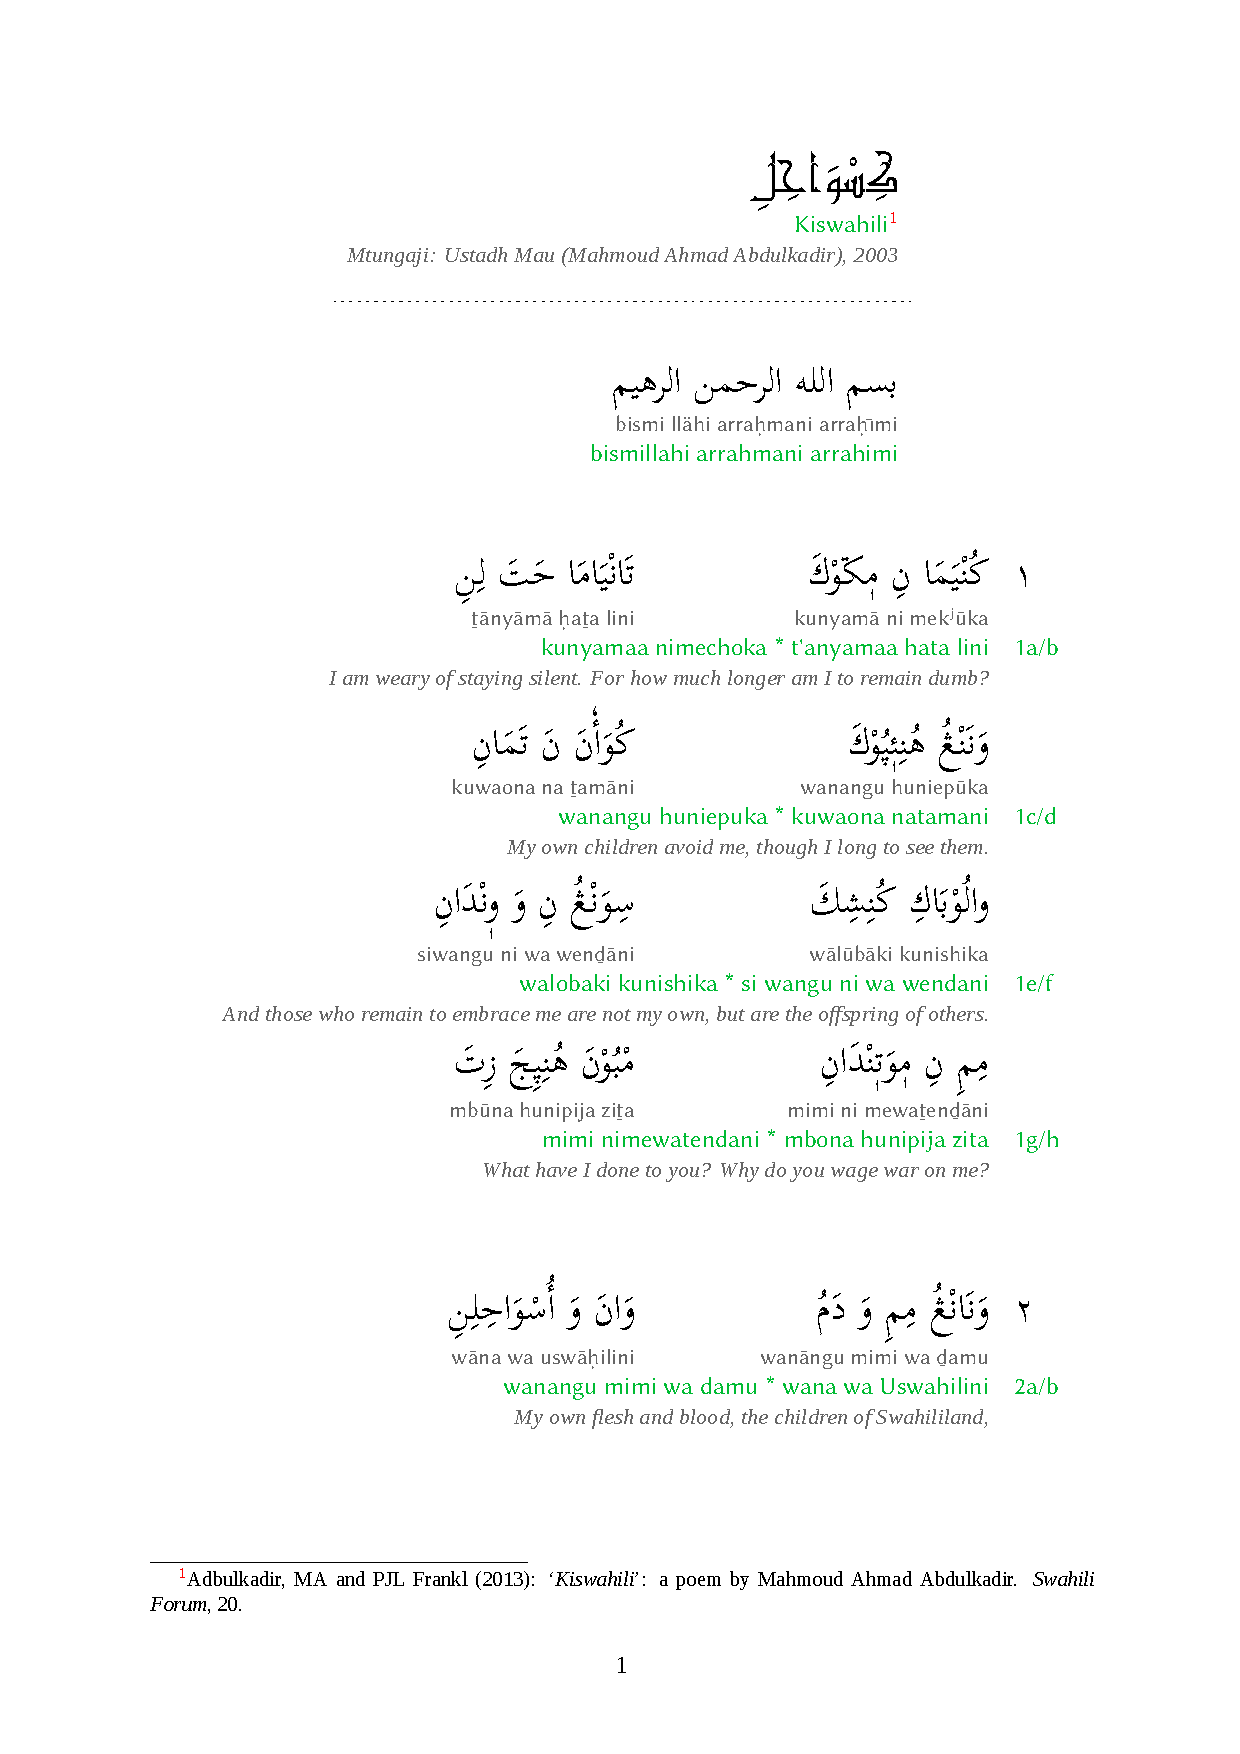
\includepdf[pages={ - }, pagecommand={}]{../poetry/outputs/kiswahili/kiswahili.pdf}
% stackoverflow.com/questions/2739159/inserting-a-pdf-file-in-latex
% tex.stackexchange.com/questions/71427/include-several-pages-of-a-pdf-without-losing-latex-document-style#71435
% use pagenumbering{gobble} when generating the pdf, so that it does not have its own pagenumbering.


\newpage


%----------------
% Appendix E: layouts/tz
%----------------
\chapter{The keyboard layout file (\textit{layout/tz})}
\renewcommand{\thesection}{E/\arabic{section}}  % redefine the section numbering
\setcounter{section}{0}  % reset counter
\label{appE}

This appendix contains the contents of the \textbf{Andika!} file \textit{layout/tz}.  Lines which begin with \textbf{//} are comment lines, intended to explain which glyphs will be output when a particular key is pressed.  For more information, see \Cref{s:changelayout}.

\begin{verbatim}

// Keyboard layout for Swahili in Arabic script.
// This file is part of the Andika! project, and is licensed under GPLv3 or later.
// Version 2014-08-12
// Andika! -- kevindonnelly.org.uk/swahili
// Kevin Donnelly (kevin@dotmon.com)

xkb_symbols "swa"
{

name[Group1] = "Swahili";

include "level3(ralt_switch)"

// 1=key, 2=Shift+key, 3=AltGr+key, 4=Shift+AltGr+key

// -------------
// ZXCV row
// -------------
key <LSGT> { [Arabic_superscript_alef, Arabic_maddaonalef, Arabic_hamzaunderalef, U0671] };
// 1 superscript alef, 2 alef with madda above, 3 alef with hamza below (vowelcarrier), 4 alef wasla
key <AB01> { [Arabic_zain, Arabic_jeh, Arabic_zah] };
// 1 zain (z), 2 jeh (zh), 3 zah (zw)
key <AB02> { [Arabic_khah] };
// 1 khah (kh)
key <AB03> { [Arabic_tcheh, U063B, U06AE] };
// 1 tcheh (ch), 2 keheh with two dots above (kj), 3 kaf with three dots below (kj)
key <AB04> { [Arabic_veh] };
// 1 veh (v)
key <AB05> { [Arabic_beh] };
// 1 beh (b)
key <AB06> { [Arabic_noon, U075D] };
// 1 noon (n), 2 ain with two dots above (g in ng')
key <AB07> { [Arabic_meem] };
// 1 meem (m)
key <AB08> { [Arabic_comma, Arabic_hamza_above, comma, leftcaret] };
// 1 comma, 2 hamza as diacritic, 3 UK comma, 4 closing angle bracket
key <AB09> { [Arabic_fullstop, Arabic_sukun, period, rightcaret] };
// 1 fullstop, 2 sukun, 3 UK fullstop, 4 opening angle bracket
key <AB10> { [Arabic_question_mark, NoSymbol, KP_Divide, question] };
// 1 question mark, 3 forward slash, 4 UK question mark

// -------------
// ASDF row
// -------------
key <AC01> { [Arabic_fatha, Arabic_alef, Arabic_hamzaonalef, Arabic_fathatan] };
// 1 fatha (short a), 2 alef (long a), 3 alef with hamza above (vowelcarrier), 4 fathatan
key <AC02> { [Arabic_seen, Arabic_sheen, Arabic_sad] };
// 1 seen (s), 2 sheen (sh), 3 sad (sw)
key <AC03> { [Arabic_dal, Arabic_thal, Arabic_dad, Arabic_ddal] };
// 1 dal (d), 2 thal (dh), 3 dad (dw), 4 ddal (alveolar dr)
key <AC04> { [Arabic_feh ] };
// 1 feh (f)
key <AC05> { [U06A0, Arabic_ghain, Arabic_gaf] };
// 1 ain with three dots above (g), 2 ghain (gh), 3 gaf (g)
key <AC06> { [Arabic_ha, Arabic_hah, Arabic_tehmarbuta, Arabic_hamza] };
// 1 ha (h), 2 hah (h), 3 tehmarbuta, 4 hamza as letter
key <AC07> { [Arabic_jeem] }; 
// 1 jeem (j)
key <AC08> { [Arabic_kaf, U06AA] };
// 1 kaf (k), 2 swash kaf (k)
key <AC09> { [Arabic_lam] };
// lam (l)
key <AC10> { [Arabic_semicolon, NoSymbol, semicolon, colon] };
// 1 semicolon, 3 UK semicolon, 4 UK colon
key <AC11> { [Arabic_ain, Arabic_shadda, quoteright, at] };
// 1 ain, 2 shadda, 3 UK single quote, 4 UK @    
key <BKSL> { [NoSymbol, NoSymbol, numbersign, asciitilde] };
// 3 UK hash, 4 UK tilde

// -------------
// QWER row
// -------------

key <AD01> { [Arabic_qaf] }; 
// 1 qaf (q)
key <AD02> { [Arabic_waw, NoSymbol, Arabic_hamzaonwaw, U06CF] };
// 1 waw (w), 3 waw with hamza above (vowel-carrier), 4 waw with dot above
key <AD03> { [U0656, Arabic_yeh, Arabic_hamzaonyeh] };
// 1 subscript alef (short e), 2 yeh (long e), 3 yeh with hamza above (vowel carrier)
key <AD04> { [Arabic_ra] };
// 1 ra (r)
key <AD05> { [Arabic_teh, Arabic_theh, Arabic_tah, Arabic_tteh] };
// 1 teh (t), 2 theh (th), 3 tah (tw), tteh (alveolar tr)
key <AD06> { [Arabic_yeh, Arabic_alefmaksura, Arabic_hamzaonyeh] };
// 1 yeh (y), 2 alef maksura, 3 yeh with hamza above (vowel carrier)
key <AD07> { [Arabic_damma, Arabic_waw, Arabic_hamzaonwaw, Arabic_dammatan] };
// 1 damma (short u), 2 waw (long u), 3 waw with hamza above (vowel-carrier), 4 dammatan
key <AD08> { [Arabic_kasra, Arabic_yeh, Arabic_hamzaonyeh, Arabic_kasratan] };
// 1 kasra (short i), 2 yeh (long i), 3 yeh with hamza above (vowel carrier), 4 kasratan
key <AD09> { [U0657, Arabic_waw, Arabic_hamzaonwaw] };
// 1 inverted damma (short o), 2 waw (long o), 3 waw with hamza above (vowel-carrier)
key <AD10> { [Arabic_peh] };
// 1 peh (p)
key <AD11> { [NoSymbol, NoSymbol, bracketleft, braceleft] }; 
// 3 UK opening square bracket, 4 UK open١ing brace
key <AD12> { [NoSymbol, NoSymbol, bracketright, braceright] };
// 3 UK closing square bracket, 4 UK closing brace

// -------------
// numeral row
// -------------
key <AE01> { [Arabic_1, NoSymbol, KP_1, exclam] };
// 1 digit 1, 3 UK digit 1, 4 UK exclamation mark
key <AE02> { [Arabic_2, NoSymbol, KP_2, quotedbl] };
// 1 digit 2, 3 UK digit 2, 4 UK double quote
key <AE03> { [Arabic_3, NoSymbol, KP_3, sterling] }; 
// 1 digit 3, 3 UK digit 3, 4 UK pound sign
key <AE04> { [Arabic_4, NoSymbol, KP_4, dollar] };
// 1 digit 4, 3 UK digit 4, 4 UK dollar sign
key <AE05> { [Arabic_5, NoSymbol, KP_5, percent] }; 
// 1 digit 5, 3 UK digit 5, 4 UK percent sign
key <AE06> { [Arabic_6, NoSymbol, KP_6, asciicircum] };
// 1 digit 6, 3 UK digit 6, 4 UK circumflex 
key <AE07> { [Arabic_7, NoSymbol, KP_7, ampersand] };
// 1 digit 7, 3 UK digit 7, 4 UK ampersand
key <AE08> { [Arabic_8, NoSymbol, KP_8, KP_Multiply] }; 
// 1 digit 8, 3 UK digit 8, 4 UK asterisk
key <AE09> { [Arabic_9, NoSymbol, KP_9, parenleft] };
// 1 digit 9, 3 UK digit 9, 4 UK opening parenthesis
key <AE10> { [Arabic_0, NoSymbol, KP_0, parenright] };
// 1 digit 0, 3 UK digit 0, 4 UK closing parenthesis
key <AE11> { [U060D, NoSymbol, KP_Subtract, underbar] };
// 1 date separator, 3 UK dash, 4 UK underscore
key <AE12> { [NoSymbol, NoSymbol, KP_Equal, KP_Add] };
// 3 UK equals sign, 4 UK addition sign

};

\end{verbatim}



\newpage


\end{document}